

%LJ changed from article to book
\documentclass[11pt]{book}
\usepackage{graphicx}
%\usepackage{stylemydefs}
%\input epsf
\usepackage{natbib}
%\usepackage{appendix}
\usepackage{bm}
\usepackage{amssymb}
\makeatletter  % Allow the use of @ in command names
\long\def\@makecaption#1#2{%
  \vskip\abovecaptionskip
  \sbox\@tempboxa{{\captionfonts #1: #2}}%
  \ifdim \wd\@tempboxa >\hsize
    {\captionfonts #1: #2\par}
  \else
    \hbox to\hsize{\hfil\box\@tempboxa\hfil}%:3355
  \fi
  \vskip\belowcaptionskip}
\makeatother   % Cancel the effect of \makeatletter
\newcommand{\captionfonts}{\small}
%\usepackage{rotating}
%\usepackage{longtable}

% for book only:
\usepackage[left=1.4in,right=1.4in,bottom=1.4in,top=1.4in]{geometry}

%\usepackage{makeidx}
%\makeindex

%\usepackage{fancyhdr}
%\pagestyle{fancy}
%\fancyhf{}
%\fancyfoot[C]{\thepage}
%\fancyhead[LO]{\bfseries\rightmark} 
%\fancyhead[RE]{\bfseries\leftmark} 
% 


% comment these out for book version
\usepackage{hyperref} 

 \begin{document}
 
%\input{customlinks} % comment these out for book version
 %\newcommand{\be}{\begin{equation}}% comment these out for book version
%\newcommand{\ee}{\end{equation}}% comment these out for book version

 % LORI:  MAKE A CUSTOM LINK EVERYWHERE I HAVE A LABEL  - I FORGOT HOW TO DO THIS....  
 
 \title{PmagPy Cookbook}
 \author{Lisa Tauxe\\Scripps Institution of Oceanography\\La Jolla, CA 92093-0220}
\today
 \maketitle

%\setcounter{tocdepth}{1}
%\tableofcontents
%\customlink{survival_skills}
\chapter{Survival computer skills}
\label{ex:unix}

The `Py' part of `PmagPy' stands for Python, the language in which all the code is written.   It is not essential, but it is helpful to understand a bit about Python when using PmagPy because no one should be using programs as black boxes without understanding what they are doing. As all the programs are open source, you have the opportunity to look into them.  If you understand a bit of Python yourself, you will be able to follow along what they are doing and even modify them to work better for you.   So in this chapter you will find a brief introduction to the computer skills necessary for using the programs properly.  

%\customlink{command_line}
\section{Finding your command line}
If you are not using a UniX like computer, you may never have encountered a command line. While the MagIC.py Graphical User Interface (GUI) is an attempt to make life as easy for you by constructing UNIX commands for you, you still need to find the command line to start it up.  Under the MacOS X operating system look for the Terminal application in the Utilities folder within the Applications folder:

  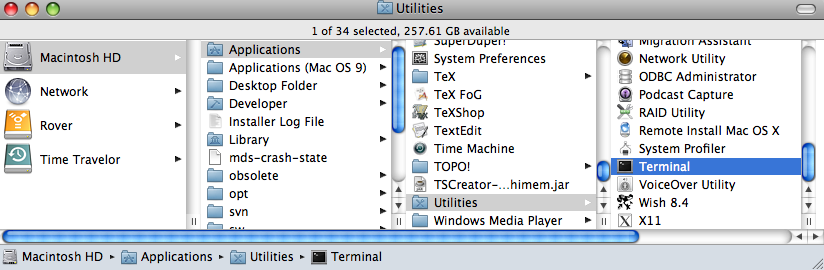
\includegraphics[width=12 cm]{EPSfiles/terminal.png}

Under the Windows operating system, find the program called: Command Prompt in the Start menu:

  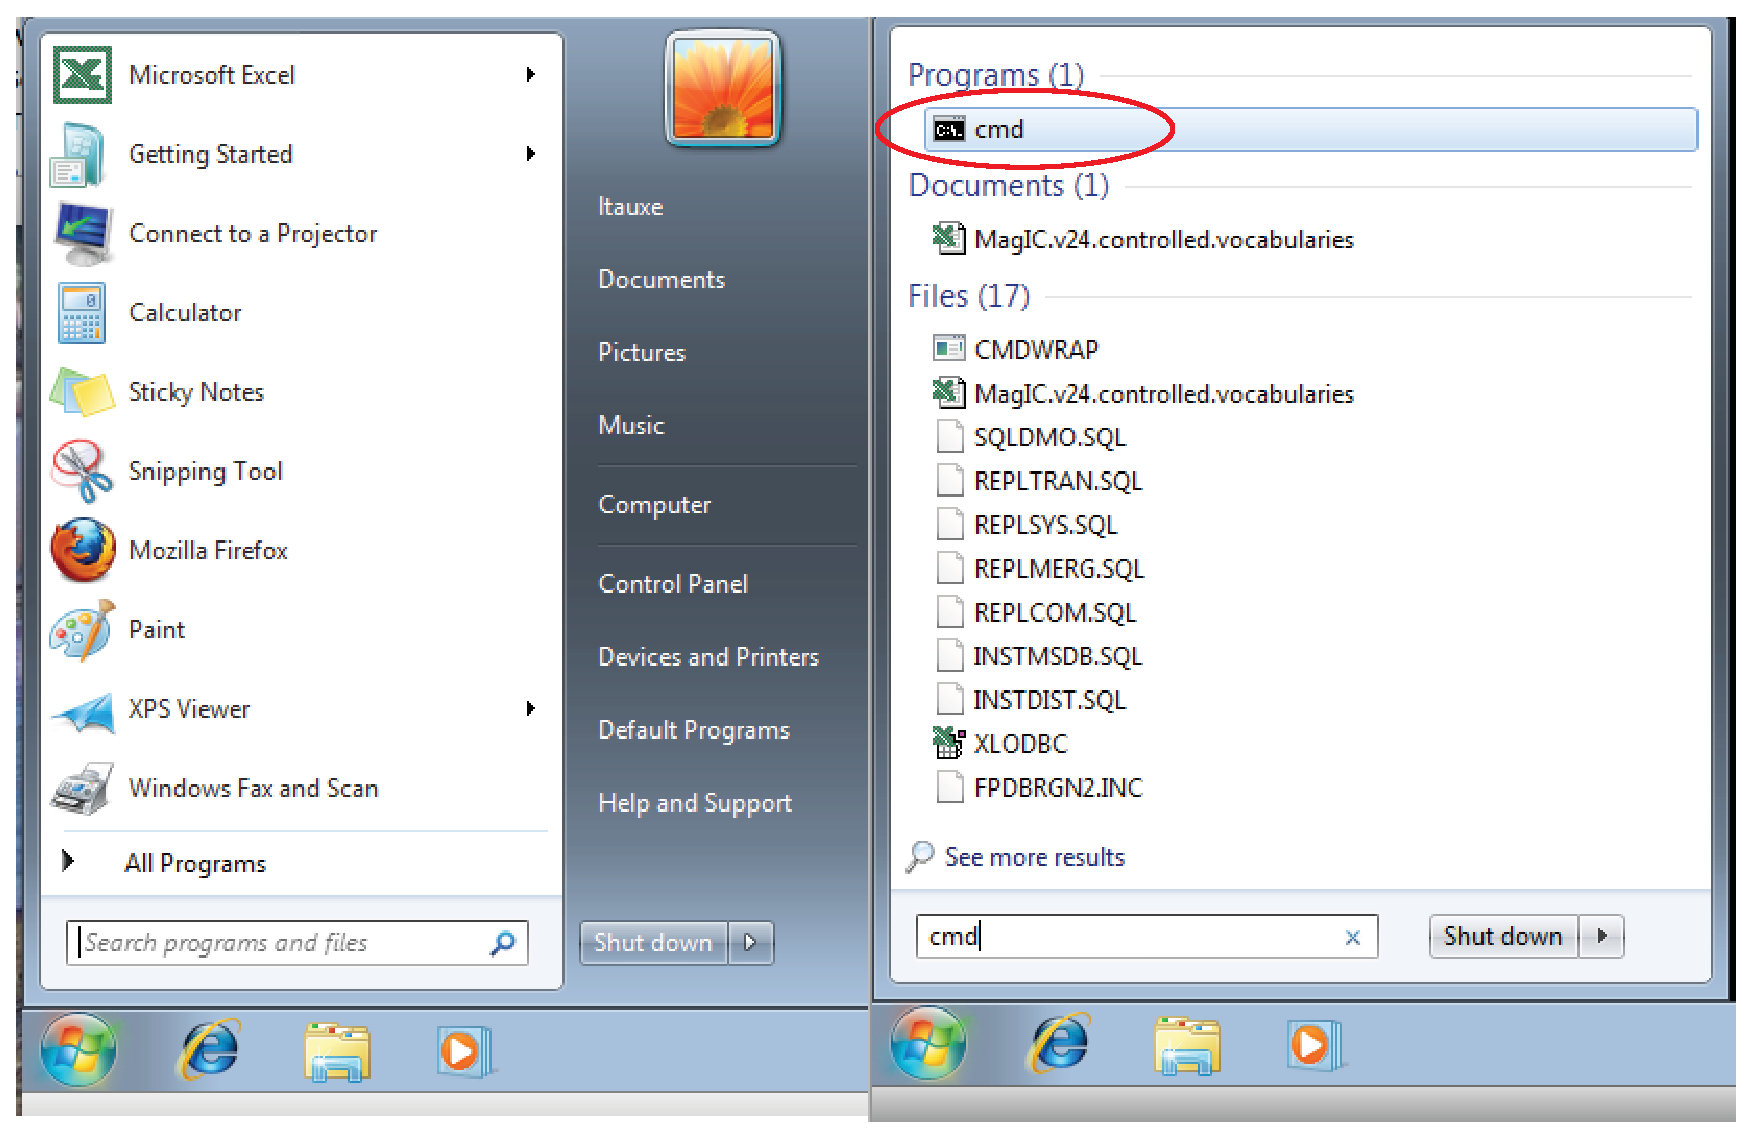
\includegraphics[width=15 cm]{EPSfiles/cmd.eps}
  
  Note that the location of this program varies on various computers, so you may have to hunt around a little to find yours. Also, the actual "prompt" will vary for different machines. The MacOS and Windows command line windows look like these:
  
    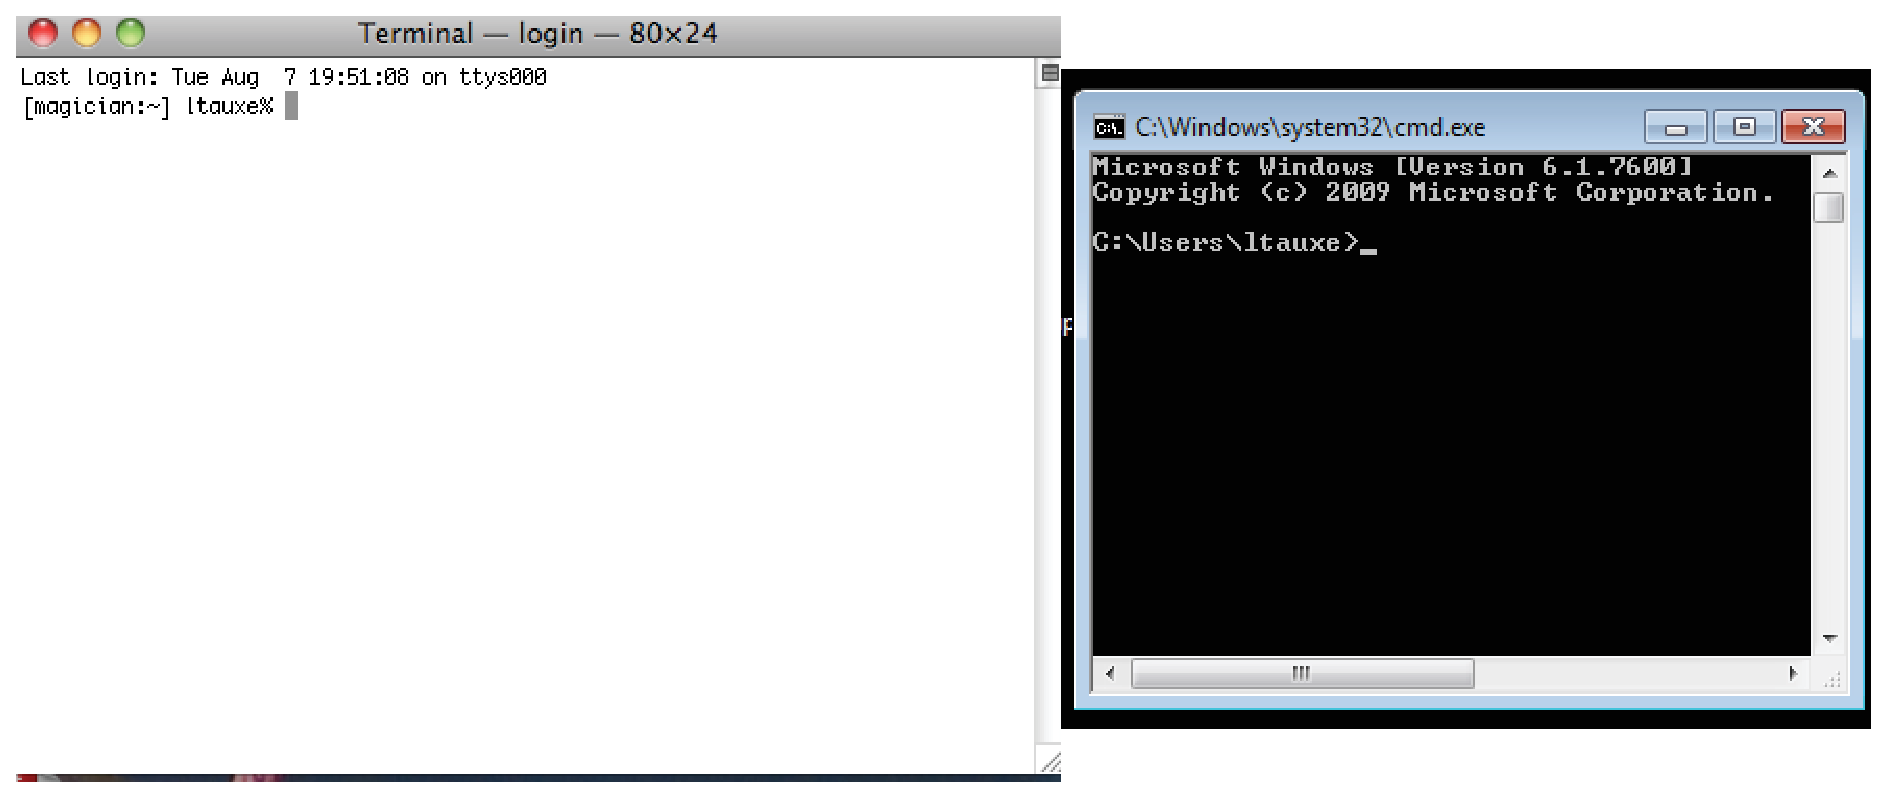
\includegraphics[width=15 cm]{EPSfiles/terminals.eps}
    

  
  
\section{File systems}
\label{sect:file_systems}
    When you open one of these,  you are working in your  ``home'' directory.   
Fundamental to all  operating systems is the concept of
directories and files.  On windows-based operating systems (MacOS or Windows), directories are depicted
as ``folders'' and moving about is accomplished by clicking on the different icons.
In the world of terminal windows, the directories have names and are arranged in a hierarchical sequence with
the top directory being the ``root'' directory, known as  ``/'' (or C:\\ in Windows) and the file system looks something like this:

  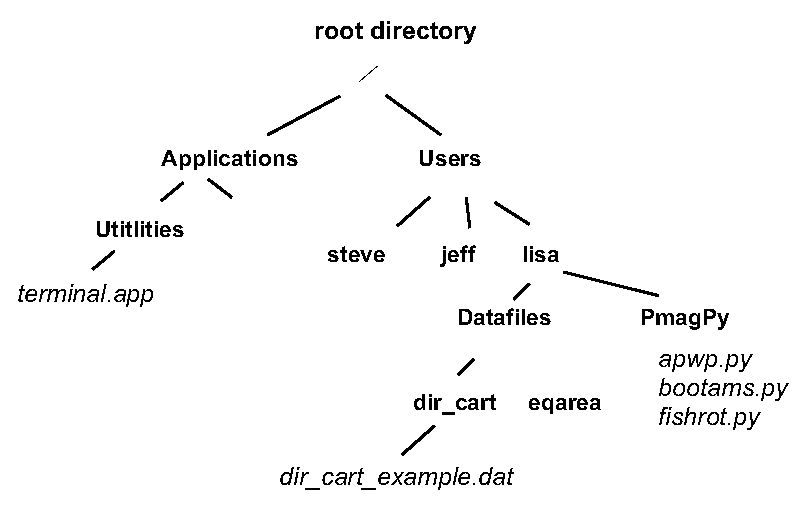
\includegraphics[width=15 cm]{EPSfiles/filesys.eps}

 Within the root directory, there are subdirectories
(e.g. {\bf Applications} and {\bf Users} in italics.  In any directory, there can also be ``files''
(e.g. {\it dir\_cart\_example.dat} in boldface).   To
refer to directories,  the operating system relies on what is called a ``pathname''. Every object
has an ``absolute'' pathname which is valid from anywhere on the computer.  The
absolute pathname in *NIX always begins from the root directory {\bf /} and in DOS (the operating system working in the Windows command line window), it is C:\\. 

The absolute pathname to the home directory {\bf lisa} in the figure is {\bf /Users/lisa}.  
Similarly, the absolute pathname to the directory containing {\bf PmagPy}  
scripts  would be  {\bf /Users/ltauxe/PmagPy}.  There is also a ``relative'' pathname,
which is in reference to the  current directory.  If user ``lisa'' is sitting in 
her home directory, the relative pathname for the file {\it dir\_cart\_example.dat} in the directory
{\it datafiles} would be {\it dir\_cart/foldtest\_example.dat}.  When using relative
pathnames, it is useful to remember that {\bf ./} refers to the current
directory and {\bf ../} refers to the directory  ``above''.     

\section{Moving around in the file system}

Now you have found your command line and are comfortable in your home directory, you can view the contents of your directory with the Unix command {\bf ls} or the DOS command {\bf dir}.  
%\customlink{mkdir}
You can make a new directory with the command {\bf mkdir NEW\_DIRECTORY\_NAME} (works in both Unix and DOS environments) and you can move into your new directory with the command {\bf cd NEW\_DIRECTORY\_NAME}.   To move back up into the home directory, just type {\bf cd ..} remembering that .. refers to the directory above.  Also, {\bf cd} by itself will transport you home from where ever you are (there's no place like home....).     You can also change to any arbitrary directory by specifying the full path of the destination directory. 



\section {Wildcards}

Unix and DOS have the ability to refer to a number of files and/or directories using
``wildcards''.  The  wildcard for a  single character is ``?'' and for any number of
characters is ``*''.  For example, to refer to all the files with ``.py'' in their name in the PmagPy directory in my home directory, 
I would type:

\begin{verbatim}
% ls PmagPy/*.py
apwp.py bootams.py fishrot.py.....
\end{verbatim}


 To refer only a single character, we use the symbol `?'. 




\section {Redirecting input and output}

Programs that operate at the command line level print  output to the screen and read input
from the keyboard. This is
known as ``standard input and output'' or ``standard I/O''.
One of the nicest things about working at the command line level is the ability to redirect input and output.
For example, instead of typing input to a program with the keyboard, it can
be read from a file using the symbol {\bf $<$}.   Output can either be put into a 
file using the symbol {\bf $>$}, appended to the end of a file with {\bf $>>$} or 
used as input to another program with the pipe facility ({\bf$ |$}).



\section{Text editors}

Text editing is a blessing and a curse.  You either love it or
hate it and in the beginning, if you are used to programs like Word, you will certainly hate it.  There are many ways of
editing text and the subject is beyond the scope of this book.   But you can't use Word because the output is in a weird format that no scripting languages don't read easily.  So you have to use an editor that will produce a plain (ascii) file, like Notepad or TextWrangler.   The latter is freeware available for Macs and the former comes standard in the Windows operating system.  

%\customlink{installing_python}
\section{Installing Python and PmagPy}
\label{sect:python}

\subsection{Installing and starting Python}


Python can  be painful to install (but so can  all other programming environments).  There are  a few recipes that work for Mac OS (at least for 10.4 and later) and for Windows.  These recipes and the ingredients are available through the website: 

\url{magician.ucsd.edu/Software/PmagPy}.



Once Python is installed and you've found your command line, you will notice a ``prompt".  
The prompt will vary for different machines and may start with a `$>$ (Windows), a '\%' (c-shell) or a `\$' (bash).  We will use a '\$'  or  a '\%' to indicate the prompt in this book.     After the command prompt, type:  {\bf python} to start the interactive python shell.  [Also, the symbol ctrl-D  means to hold down the control key while typing the letter ``d''.  On Windows machines, you may have to substitute a letter ``c'' to achieve the same effect. ]

 Everyone should now have the $>>>$ prompt.  Here is a transcript of a python interpreter session which should make a simple graph:  
 
 \begin{verbatim}
% python
Enthought Python Distribution -- www.enthought.com
Version: 7.1-2 (32-bit)

Python 2.7.2 |EPD 7.1-2 (32-bit)| (default, Jul 27 2011, 13:29:32) 
[GCC 4.0.1 (Apple Inc. build 5493)] on darwin
Type "packages", "demo" or "enthought" for more information.
>>> import matplotlib
>>> import pylab
>>> pylab.plot([1,2,3,4])
[<matplotlib.lines.Line2D object at 0x64eb270>]
>>> pylab.show()

\end{verbatim}

which produces the fascinating graph:

  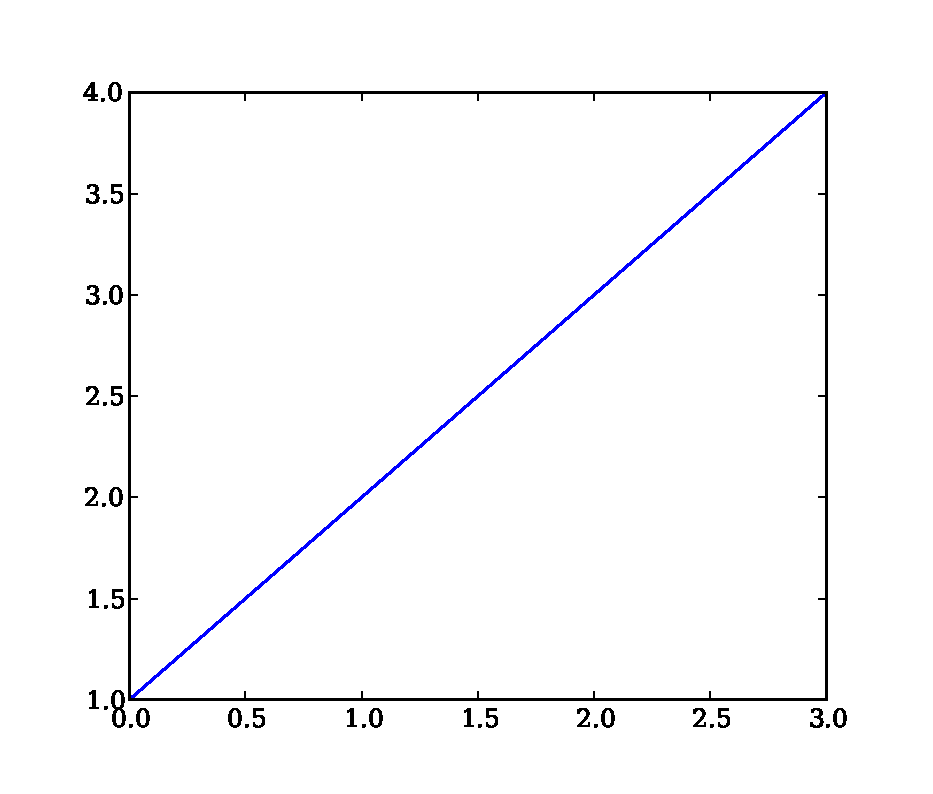
\includegraphics[width=12 cm]{EPSfiles/matplotlib.eps}


To kill the interpreter, close the plot window (red button) and type ctrl-D.  


If you don't get something about Enthought Python, you are probably using the standard Mac Os version, which has none of the whistles and bells we want (plotting, numerical packages, etc.), you'll need to set your path properly. Look for hints at:
\url{http://magician.ucsd.edu/Software/Python}.    


\section{Introduction to Python Programming}



As you have just fired up Python, you are in an interactive mode with the prompt  {\color{blue}$>>>$}.  Like Matlab, you can just start typing commands. After each command, press the return key and see what happens:

{ \color{blue} \begin{verbatim}
>>> a=2 
>>> a
2
>>> b=2
>>> c=a+b
>>> c
>>> c+=1
>>> c
5
>>> a=2; b=2; c=a+b; c
4
>>> d,e,f=4,5,6 # note syntax! d=4;e=5;f=6
>>> # note also that the symbol '#' means the rest of the line is a comment!
\end{verbatim}}

To get out of Python interactive mode and back to your beloved command line, type the control key (here-after  {\color{blue}\^{ }}) and  {\color{blue}D} at the same time.  PC users may have to type {\color{blue} \^{ }C} instead. 

From your Fortran programming experience, you will recognize $a, b,$ and $c$ in the above session as {\it variables} and $+$ as an {\it operation}. You may have been surprised that we didn't declare variables up front (C programmers always have to).  And, the variables above are obviously behaving as integers, not floating point variables (no decimals) but they are not letters between $i$ and $n$.  And there were funny lines that seemed to set three numbers at once:

{ \color{blue} \begin{verbatim}
>>> a=2; b=2; c=a+b; c
and
>>> d,e,f=4,5,6 # note syntax! d=4;e=5;f=6
\end{verbatim}}
\noindent
Here are some rules governing variables and operations in Python:


\begin{itemize}
\item Variable names are composed of alphanumeric characters, including `-` and '\_'.
\item They are case sensitive:  `a' is not the same as 'A'.
\item They do NOT have to be specified in advance (unlike C)
\item In fortran, integers are  $i-n$ and floating points are all else - not the case in Python. You can make them whatever you want.  
\item + adds, - subtracts, * multiplies, / divides, \% gives the remainder, ** raises to the power
\item These two are fun: {\color{blue}+=} and  {\color{blue}-=}.  They increment and decrement respectively. 
\item Parentheses determine order of operation (as in Fortran). 
\item  For math functions, we can use various modules that either come standard with python (the math module) or are additions that come with the Enthought Python Edition we are using (the NumPy module).  A module is just a collection of functions. NB:  There is online help for any python function or method:  just type help(FUNC). 
\end{itemize}


\section{A first look at NumPy}

O.K.  First of all - how do you pronounce `NumPy'.  According to Important People at Enthought (e.g, Robert Kern), it should be pronounced ``Num'' as in ``Number'' and ``Pie'' as in, well, pie, or Python.  Oops.  It is way more fun to say Numpee!

So, that out of the way, what can NumPy do for us?  Turns out, a whole heck of a lot!  But for now we will just scratch the surface.   It can, for example, give us the value of $\pi$ as {\color{blue}numpy.pi}.  Note how the module name comes first, then the name of the function we wish to use.  In this case, the function just returns the value of $\pi$.  

To use {\color{blue}NumPy} functions, we must first ``import'' the module with the command {\color{blue}import}.  The first time you do this after installing Python, it may take a while, but after that it should be very quick.  

There are four styles of the import command which all do pretty much the same thing but differ in how you have to call the function after importing: 

{ \color{blue} \begin{verbatim}
>>>  import numpy
>>> numpy.pi
3.1415926535897931
\end{verbatim}}
\noindent
This makes all the functions in NumPy available to you, but you have to call them with the {\color{blue}numpy.FUNC} syntax.

{ \color{blue} \begin{verbatim}
>>>  import numpy as np  # or anything else!  e.g., some use:  N
>>> np.pi  # or N.pi in the second case.
3.1415926535897931
\end{verbatim}}
\noindent
This does the same as the first, but allows you to call NumPy anything you want - to save typing?
\noindent
To import all the functions from NumPy and not have to type numpy at all: 
{ \color{blue} \begin{verbatim}
>>> from numpy  import *
>>> pi
3.1415926535897931
\end{verbatim}}
\noindent
This imports all the umpty-ump functions, which is a heavy load on your memory,  but you can also just import a few, like {\color{blue}pi} or {\color{blue}sqrt}:
{ \color{blue} \begin{verbatim}
>>> from numpy import pi, sqrt # pi and square root
>>> pi
3.1415926535897931
>>> sqrt(4)
2.0
\end{verbatim}
}
\noindent
Did you notice how {\color{blue}sqrt(4)} where 4 was an integer, returned a floating point variable (2.0)?  

{\color{magenta}Good housekeeping Tip \#1:  I tend to import modules using the first option above.  That way  I know what module the functions I'm using are coming from - especially because we don't know off-hand ALL the functions available in any given module and there might be conflicts with my own function names or two different modules could have the same function (like} {\color{blue}math} {\color{magenta}and }{\color{blue}numpy}).  


Here is a (partial) list of some useful {\color{blue}NumPy} functions:


\begin{tabular}{ll}
\hline
absolute(x)  & absolute value\\
arccos(x)    & arccosine\\
arcsin(x)    & arcsine\\
arctan(x)    & arctangent\\
arctan2(y,x)  &arctangent of y/x in correct quadrant (***very useful!)\\
cos(x)        &cosine\\
cosh(x)      & hyperbolic cosine\\
exp(x)      &  exponential\\
log(x)      &  natural logarithm\\
log10(x)    &  base 10 log\\
sin(x)       & sine\\
sinh(x)     &  hyperbolic sine\\
sqrt(x)    &   square root\\
tan(x)      &  tangent\\
tanh(x)    &   hyperbolic tangent\\
\hline
\end{tabular}

\noindent 
Note that  in the trigonometric functions,  the argument is in RADIANS!.You can convert from degrees to radians by multiplying by:  {\color{blue}numpy.pi/180.}.  Also notice how these functions have parentheses, as opposed to {\color{blue}numpy.pi} which has none.  The difference is that these take arguments, while  {\color{blue}numpy.pi} just returns the value of $\pi$.  


\noindent 
If you are desperate, you can always use your Python interpreter as a calculator:

{ \color{blue} \begin{verbatim}
>>> import numpy
>>> a=2
>>> b=-12
>>> c=16
>>> quad1 = (-b + numpy.sqrt(b**2-4.*a*c))/(2.*a)
>>> quad1
4
>>> y=numpy.sin(numpy.pi/6.)
>>> y
0.5
\end{verbatim}}


\section{Variable types}

The time has come to talk about variable types.  We've been very relaxed up to now, because we don't have to declare them up front and we can often even change them from one type to another on the fly.  But - variable types matter, so here goes.  Like Fortran, Python has integer, floating point (both long and short), string and complex variable types.  It is pretty clever about figuring out what is required.   Here are some examples:

{ \color{blue} \begin{verbatim}
>>> number=1 # an integer
>>> Number=1.0 # a floating point
>>> NUMBER='1' # a string
>>> complex=1j # a complex number with imaginary part 1
>>> complex(3,1) # the complex number 3+1i 
\end{verbatim}}
\noindent
{Try doing math with these!}
{ \color{blue} \begin{verbatim}
>>> number+number
2     [ an integer]
>>> number+Number
2.0   [ a float]
>>> NUMBER+NUMBER
11 [a string]
>>> number+NUMBER  [Gives you an angry error message]
\end{verbatim}}
\noindent
 Lesson learned: you can't add a number and a string.  and string addition is different!  But you really have to be careful with this.  If you multiply a float by an integer, it is possible that you will convert the float to an integer when you really wanted all those numbers after the decimal! So, if you want a float, use a float.  
 
{ You can convert from one type to another (if appropriate) with:}
{ \color{blue} \begin{verbatim} 
 int(Number); str(number);  float(NUMBER); 
 long(Number); complex(real,imag)
 \end{verbatim}}
 
\noindent 
{\color{blue}long()} converts to a double precision floating point and {\color{blue}complex()} converts the two parts to a complex number.
 
 There is another kind of variable called ``boolean''. These are: {\color{blue}true}, {\color{blue}false}, {\color{blue}and}, {\color{blue}or}, and {\color{blue}not}
For the record, the integer  `1' is {\color{blue}true} and  `0' is {\color{blue}false}.  
These can be used to control the flow of the program as we shall learn later.  

\section{Data Structures}

In Fortran, you encountered arrays, which was a nice way to group a sequence of numbers that belonged together.  In Python of course we also have arrays, but we also have more complicated data structures, like lists, tuples, and dictionaries,  that group arbitrary variables together, like strings and integers and floats - whatever you want really. We'll go through some attributes of the various data structures, starting with lists.

\subsection{Lists}
%%\vskip -.25in
\begin{itemize}
\item Lists are denoted with []  and can contain any arbitrary set of items, including other lists!
\item Items in the list are referred to by an index number, starting with 0.  Note that this is different from Fortran which starts counting in arrays with the number 1.
\item You can  count from the end to the beginning by starting with -1 (the last item in the list), -2 (second to last), etc. 
\item Items can be sorted, deleted, inserted, sliced, counted, concatenated, replaced, added on, etc.
\end{itemize}
\noindent
Examples:

{ \color{blue} \begin{verbatim}
>>> mylist=[`a',2.0,`400',`spam',42,[24,2]] # defines a list
>>> mylist[2] # refers to the third item
`400'
>>> mylist[-1] # refers to the last item
[24,2]
>>> mylist[1]=26.3   # replaces the second item
>>> del mylist[3] # deletes the fourth element 
\end{verbatim}}


\noindent
To slice out a chunk of the middle of a list:
{ \color{blue} \begin{verbatim}
>>> newlist=mylist[1:3]
\end{verbatim}}
\noindent
This takes items 2 and 3 out (note it takes out up to but not including the last item number - don't ask me why).  
Or, we can slice it this way:
{ \color{blue} \begin{verbatim}
>>> newlist=mylist[3:] 
\end{verbatim}}
\noindent
which takes from the fourth item (starting from 0!) to the end. 


To copy a list BEWARE! You can make  a copy - but it isn't a copy like in Fortran, but it is just another name for the SAME OBJECT, so:
{ \color{blue} \begin{verbatim}
>>> mycopy=mylist
>>>mylist[2]=`new'
>>>mycopy[2]
`new'
\end{verbatim}}
\noindent
See how mycopy got changed when we changed mylist?
\noindent
To spawn a new list that is a copy, but an independent entity:
{ \color{blue} \begin{verbatim}
>>>mycopy=mylist[:]
\end{verbatim}}
\noindent
Now try:
{ \color{blue} \begin{verbatim}
>>>mylist[2]=1003
>>>mycopy[2]
`new'
\end{verbatim}}
\noindent
So now {\color{blue}mycopy}  stayed the way it was, even as {\color{blue}mylist } changed.  


Unlike Fortran, Python is ``object oriented'', a popular concept in coding circles.  We'll learn more about what that means later, but for right now you can walk around feeling smug that you are learning an object oriented programming language.   O.K., what is an object?  Well, 
{\color{blue}mylist} is an object.   Cool.  What do objects have that might be handy?  
Objects have ``methods'' which allow you to do things to them.  Methods have the form:
{\color{blue}object.method()}

\noindent
Here are two examples:

{ \color{blue} \begin{verbatim}
>>> mylist.append(`me too') # appends a string to mylist
>>> mylist.sort() # sorts the list alphanumerically
>>> mylist
[2.0, 42, [24, 2], '400', 'a', 'me too', 'spam']
\end{verbatim}}
%%\vskip .25in


\noindent

 For a complete list of methods for lists, see:
http://docs.python.org/tutorial/datastructures.html\#more-on-lists

\subsection{More about strings}
Numbers are numbers. While there are more kinds of numbers (complex, etc.),
strings can be  more interesting. Unlike in Fortran, they can be denoted with single, double or triple quotes:  e.g.,
`spam',  ``Sam's spam'', or
{ \color{blue} \begin{verbatim}
"""  
Hi there I can type as
many lines as I want
"""
\end{verbatim}}

Strings can be added together ({\color{blue}newstring = 'spam' + 'alot'}).  They  can be sliced ({\color{blue}newerstring = newstring[0:3]}). 
but they CANNOT be changed in place - you can't do this: {{\color{blue}newstring[0]='b'}.
To find more of the things you can and cannot do to strings, see: http://docs.python.org/tutorial/introduction.html\#strings

\subsection{Data structures as objects}



\subsection{Tuples}
What?  Tuples?  
Tuples consist of a number of values separated by commas.  They are denoted with parentheses. 
{ \color{blue} \begin{verbatim}
>>> t = 1234, 2.0, `hello'
>>> t
(1234, 2.0, `hello')
>>> t[0]
1234
\end{verbatim}}

\noindent Tuples are sort of like lists, but like strings, their elements cannot be changed.  However, you can slice, concatenate, etc.
 For more see: 
 
 http://docs.python.org/tutorial/datastructures.html\#tuples-and-sequences




\subsection {Dictionaries!}

Dictionaries are denoted by \{\}.  They are also somewhat like lists, but instead of integer indices, they use alphanumeric `keys':
I love dictionaries.  So here is a bit more about them.

\noindent
To define one: 
{ \color{blue} \begin{verbatim}
>>> Telnos={`lisa':46084,`lab':46531,`jeff':44707} # defines a dictionary
\end{verbatim}}

\noindent
To return the value associated with a specific key:
{ \color{blue} \begin{verbatim}
>>> Telnos[`lisa']
46084
\end{verbatim}}

\noindent
 To change a key value:

{ \color{blue} \begin{verbatim}
>>> Telnos['lisa']=46048
\end{verbatim}}


\noindent
To add a new key value:
{ \color{blue} \begin{verbatim}
>>> Telnos[`newguy']=48888
\end{verbatim}}


\noindent
 Dictionaries also have some methods.
One useful one is:
{ \color{blue} \begin{verbatim}
>>> Telnos.keys()
[`lisa',`lab',`jeff',`newguy']
\end{verbatim}}

\noindent
which returns a list of all the keys.  

For a more complete accounting of dictionaries,  see: 

http://docs.python.org/tutorial/datastructures.html\#dictionaries



\subsection{N-dimensional arrays}

Arrays  in Python  have many similarities  to  lists.
Unlike lists, however,  arrays have to be all of the same data type (dtype), usually numbers (integers or floats), although there appears to be something called a character array.  Also, the size and shape of an array must be known {\it a priori} and not determined on the fly like lists. For example we can define a list with {\color{blue}L=[]}, then append to it as desired, but not so arrays - they are much pickier and we'll see how to set them up later.  

Why use arrays when you can use lists?  They are far more efficient than lists particularly for things like matrix math.   But just to make things a little confusing, there are  several different data objects that are loosely called arrays, e.g., arrays, character arrays and matrices.  These are all subclasses of ndarray.  I'm just going to briefly introduce arrays and matrices here.  

 Here are a few ways of making arrays:  
%%\vskip -.35in
{ \color{blue} \begin{verbatim}
>>> import numpy
>>> A= numpy.array([[1,2,3],[4,2,0],[1,1,2]])
>>> A
array([[1, 2, 3],
       [4, 2, 0],
       [1, 1, 2]])
>>> B=numpy.arange(0,10,1).reshape(2,5)
>>> B
array([[0, 1, 2, 3, 4],
       [5, 6, 7, 8, 9]])
>>> C=numpy.array([[1,2,3],[4,5,6]],numpy.int32) 
>>> C
array([[1, 2, 3],
       [4, 5, 6]])
>>> D=numpy.zeros((2,3)) # Notice the zeros and the size is specified by a tuple.
>>> D
array([[ 0.,  0.,  0.],
       [ 0.,  0.,  0.]])
>>> E=numpy.ones((2,4))
>>> E
array([[ 1.,  1.,  1.,  1.],
       [ 1.,  1.,  1.,  1.]])
>>> F=numpy.linspace(0,10,14)
>>> F
array([  0.        ,   0.76923077,   1.53846154,   2.30769231,
         3.07692308,   3.84615385,   4.61538462,   5.38461538,
         6.15384615,   6.92307692,   7.69230769,   8.46153846,
         9.23076923,  10.        ])      
>>> G=numpy.ndarray(shape=(2,2), dtype=float) 
>>> G   # note how this is initalized with really low numbers (but not zeros).
array([[  1.90979621e-313,   2.75303490e-308],
       [  1.08539798e-071,   3.05363949e-309]])         
\end{verbatim}}

Note the difference between {\color{blue}linspace(start,stop,N)} and {\color{blue}arange(start,stop,step)}. The function {\color{blue}linspace} creates an array with 14 evenly spaced elements between the start and stop values while  {\color{blue}arange} creates an array with elements at {color{blue}step} intervals between the starting and stopping values.    In some of the online examples you will find the short-cuts for {\color{blue}arange()} and {\color{blue}linspace} as  {\color{blue}r\_(-5,5,20j)} and {\color{blue}r\_(-5,5,1.)} respectively.

Python arrays have methods like {\color{blue}dtype},  {\color{blue}ndim}, {\color{blue}shape}, {\color{blue}size}, {\color{blue}reshape()}, {\color{blue}ravel()},  {\color{blue}transpose()} etc.    Did you notice how some of these require parentheses and some don't? The answer is that some of these are functions and some are classes, both of which we will get to later.  

Let's see what the methods can do. 
First,  arrays made in the above example are of different data types. To find out what data type an array is, just use the method {\color{blue}dtype} as in:

{ \color{blue} \begin{verbatim}
>>> D.dtype
dtype('float64')
>>>
\end{verbatim}}



 And of course  arrays, unlike lists have dimensions and shape.  Dimensions tell us how many axes there are with axes defined as in this illustration:

   \includegraphics[width=4in]{EPSfiles/ndim.eps} 
   
   As shown above our {\color{blue}A} array has two dimensions (axis 0 and 1).  To get Python to tell us this, we use the {\color{blue}ndim} method:
   
   { \color{blue} \begin{verbatim}
>>>  A= numpy.array([[1,2,3],[4,2,0],[1,1,2]]) # just to remind you
>>> A.ndim
2
\end{verbatim}}
Notice how {\color{blue}zeros, ones} and {\color{blue}ndarray} used a shape tuple in order to define the arrays in the examples above.   The shape of an array is how many elements are along each axis.  So, naturally we see that the C array is a 2x3 array.  Python returns a tuple with the shape information using the {\color{blue}shape} method:
{ \color{blue} \begin{verbatim}
>>> C.shape
(2, 3)
\end{verbatim}}

Let's say we don't want a 2x3 array for the sequence in the array {\color{blue}C}, but we want a 3x2 array.  Python can reshape an array with a different shape tuple like this:
   { \color{blue} \begin{verbatim}
>>> C.reshape((3,2))
array([[1, 2],
       [3, 4],
       [5, 6]])
\end{verbatim}}

And sometimes we just want all the elements lined up along one axis. We could do that with {\color{blue}reshape} of course using a tuple  with the size of the array (the total number of elements). You  can see that this is 6 here. We could even get python to tell us what the size is ({\color{blue}C.size}) and use that in the reshape size tuple.  Alternatively we can use the {\color{blue}ravel()} method which doesn't require us to know the size in advance:

   { \color{blue} \begin{verbatim}
>>> C.ravel()
array([1, 2, 3, 4, 5, 6])
\end{verbatim}}   

There are other ways to reshape, slice and dice arrays.  
The syntax for slicing of arrays is similar to that for lists:  
{ \color{blue} \begin{verbatim}
>>> B=A[0:2] # carve the top two lines off of matrix A from above
array([[1, 2, 3],
       [4, 5, 6]])
\end{verbatim}}

Lots of applications in Earth Science require the transpose of an array:
{ \color{blue} \begin{verbatim}
>>> A.transpose() # this is the same as A.T  
array([[1, 4, 7],
       [2, 5, 8],
       [3, 6, 9]])
\end{verbatim}}

Also, we can concatenate two arrays together with the - you guessed it - {\color{blue}concatenate()} method.   For a lot more tricks with arrays, go to the NumPy Reference website here:  \url{http://docs.scipy.org/doc/numpy/reference/}.   


To convert the {\color{blue}A} array to a list:   {\color{blue}L=A.tolist()},  from a list or tuple to an array:   {\color{blue}A=numpy.array(L)}, or from a list, a tuple or an array to a NumPy array:   {\color{blue}a=numpy.asarray(L))}

\subsection {More on slicing with arrays}



First a review of lists.   You will recall that in  python, indexing starts with 0, so for the list {\color{blue} L=[0,2,4,6,8], L[1]} is 2. The index of the last item is -1, so  {\color{blue}L[-1]}=8.  To find out what the index for the number 4 is, for example, we have the {\color{blue}index()} method:  {\color{blue}L.index(4}), which will return the number 2. We actually already used this method when we implemented command line arguments, but it wasn't really explained.   We know that to reassign a given index a new value we use the syntax {\color{blue}L[1]=2.5}.  
And to use a part of a list (a slice) we use, e.g.,    {\color{blue}B=L[2:4]}, which  defines  {\color{blue}B} as a list with  {\color{blue}L}'s elements 2 and 3 (4 and 6).  And you also know that  {\color{blue}B=L[2:]} takes all the elements from 2 to the end.  
From these examples, you can infer that the basic syntax for slicing is  {\color{blue}[start:stop:step]}; if the step is omitted it is assumed to be 1.  

Arrays (and matrices) work in a similar fashion to lists, but these are multidimensional objects, so things get hairy fast.
The basic syntax is the same:  {\color{blue}[start:stop:step]},  or  {\color{blue}i:j:k}.   but with Python arrays, we step through all the  {\color{blue}j}'s for each  {\color{blue}i}  at step  {\color{blue}k}.  This is best shown with examples:


{ \color{blue} \begin{verbatim}
>>> import numpy
>>> A=numpy.linspace(0,29,30)
>>> B=A.reshape(5,6)
array([[  0.,   1.,   2.,   3.,   4.,   5.],
       [  6.,   7.,   8.,   9.,  10.,  11.],
       [ 12.,  13.,  14.,  15.,  16.,  17.],
       [ 18.,  19.,  20.,  21.,  22.,  23.],
       [ 24.,  25.,  26.,  27.,  28.,  29.]])
>>> B[1:3,:-1:2] 
array([[  6.,   8.,  10.],
       [ 12.,  14.,  16.]])
\end{verbatim}}

Let's pick about the statement {\color{blue}B[1:3,:-1:2]} to see if we can understand what it does.  The first part alone returns lines 2 and 3:
{ \color{blue} \begin{verbatim}
>>> B[1:3]
array([[  6.,   7.,   8.,   9.,  10.,  11.],
       [ 12.,  13.,  14.,  15.,  16.,  17.]])
\end{verbatim}}

Here  {\color{blue}j} goes from [:-1], in other words, we all but the last element:

{ \color{blue} \begin{verbatim}
>>> B[1:3,:-1]
array([[  6.,   7.,   8.,   9.,  10.],
       [ 12.,  13.,  14.,  15.,  16.]])
\end{verbatim}}

\noindent And finally, we have the step of 2, which takes every other element:

{ \color{blue} \begin{verbatim}
>>> B[1:3,:-1:2] 
array([[  6.,   8.,  10.],
       [ 12.,  14.,  16.]])
\end{verbatim}}

\noindent For more on array slicing (indexing), see:

http://docs.scipy.org/doc/numpy/reference/arrays.indexing.html




\subsection{Looping through arrays}

 Earlier in the course, we learned that  {\color{blue} for} loops with lists  just step through item by item.  In n-dimensional arrays, they steps through row by row (like in slicing).  For example, 
 

{ \color{blue} \begin{verbatim}
>>> for r in B:
...    print r
... 
[ 0.  1.  2.  3.  4.  5.]
[  6.   7.   8.   9.  10.  11.]
[ 12.  13.  14.  15.  16.  17.]
[ 18.  19.  20.  21.  22.  23.]
[ 24.  25.  26.  27.  28.  29.]
\end{verbatim}}

If you really want to step through element by element, you can use the {\color{blue}ravel()} method which flattens an N-dimensional array to a single dimension:

{ \color{blue} \begin{verbatim}
>>> for e in B.ravel():
...    print  e
... 
0.0
1.0
2.0
3.0
etc.
\end{verbatim}}

For more on looping (or iterating), see:

\url{http://docs.scipy.org/doc/numpy/reference/arrays.nditer.html}



\section{Python Scripts}

Are you tired of typing yet? Python scripts are programs that can be run and re-run from the command line.
You can type in the same stuff you've been doing interactively into a script file (ending in .py). You can edit scripts with your favorite text editor (NOT Word!).   And then you can run them like this:

{ \color{blue} \begin{verbatim}
%python < myscript.py
\end{verbatim}}

On a Mac or Unix system,  you can put in a header line identifying the script as python (\#!/usr/bin/env python), make  it executable (chmod a+x)  and   run it like this:

{ \color{blue} \begin{verbatim}
% myscript.py
\end{verbatim}}

On PCs, you can just type the name of the script without the header or the chmod command.   But, because PCs don't come standard with a {\bf cat} command, you have to create the file with Notepad, instead of with {\bf cat} for all the examples using {\bf cat}.  

Here is an example that creates a script using the Unix {\bf cat} command, makes it executable and then runs it:

{ \color{blue} \begin{verbatim}
% cat > printmess.py
#!/usr/bin/env python
# simple Python test program (printmess.py)
print 'test message'
^-D
% chmod a+x printmess.py
% ./printmess.py
test message
\end{verbatim}}

\noindent
In a Python script on Unix machines (including MacOS), the  first line MUST be: 

{ \color{blue} \begin{verbatim}
#! /usr/bin/env python
\end{verbatim}}

\noindent
so that the file is interpreted as Python.  Unlike Fortran or C, you CANNOT start with a
comment line (try switching lines 1 and 2 and see what happens). 

The second line is a comment line.  Anything to the right of \# is assumed to be a comment
(Remember that in Fortran {\color{blue}! } serves the same function).

Notice that print goes by default to your screen.  Because the message is a string, you can use single or double quotes
for the test message.  You can get an apostrophe in your output by using double quotes
and quote marks by using single quotes, i.e.,

{ \color{blue} \begin{verbatim}
#! /usr/bin/env python
# simple Python test program 2 (printmess2.py)
print "The pump don't work 'cuz the vandals took the handles"
print 'She said "I know what it\'s like to be dead"'
\end{verbatim}}

\noindent
produces:

{ \color{blue} \begin{verbatim}
% ./printmess2.py
The pump don't work 'cuz the vandals took the handles
She said "I know what it's like to be dead"
%
\end{verbatim}}

\noindent
In the second print statement, the $\backslash$' is necessary to prevent an error (try it).   This is an example of a Python `escape code'.   These are used to escape some special meaning, as in an end-quote for a string in this example. We use the backslash to say that we really really want a quote mark here.   Other escape codes are listed here:  

\url{http://www.python-course.eu/variables.php}

Here's another example of a program - this one has an typo in line 4:

{ \color{blue} \begin{verbatim}
#! /usr/bin/env python
abeg = 2.1
aend = 3.9
adif = aend - abge
print 'adif = ', adif
\end{verbatim}}

\noindent
You had intended to type 'abeg' but typed 'abge' instead.  When
you run the program, you get an error message:

{ \color{blue} \begin{verbatim}
Traceback (most recent call last):
  File "./undeclared.py", line 4, in <module>
    adif = aend - abge
NameError: name 'abge' is not defined
\end{verbatim}}

\noindent
Error messages are a desirable feature of Python.  You don't want the program
to run by assigning some arbitrary value to abge and giving you
a wrong answer.  Yet many languages will do exactly that, including
Fortran (we can avoid this potential problem in Fortran by using the 
'implicit none' statement at the beginning our our programs).


\section{A first look at code blocks}
Any reasonable programming language must provide a way to group blocks of code together, to be executed under certain conditions.  In Fortran, for example, there are if statements and do loops which are bounded by the statements if, endif and do, endo respectively.  Many of these programs encourage the use of indentation to make the code more readable, but do not require it.  In Python, indentation is the way that code blocks are defined - there are no terminating statements. Also, the initiating statement terminates in a colon.  The trick is that all code indented the same number of spaces (or tabs) to the right belong together.  The code block terminates when the next line is less indented.     A typical Python program looks like this: 

{ \color{blue}\begin {verbatim}
program statement
block 1 top statement:
    block 1 statement
    block 1 statement \
        ha-ha i can break the indentation convention!
    block 1 statement
    block 2 top statement:
        block 2 statement
        block 2 statement
        block 3 top statement:
            block 3 statement
            block 3 statement
            block 4 top statement: block 4 single line of code
        block 2 statement
        block 2 statement
    block 1 statement
    block 1 statement
program statement
\end{verbatim}}


\noindent Exceptions to the code indentation rules are:
\begin{itemize}
\item  Any statement can be continued on the next line with the continuation character $\backslash$ and the indentation of the following line is arbitrary.  \item If a code block consists of a single statement, then that may be placed on the same line as the colon. 
\item The command {\color{blue}break} breaks you out of the code block. Use with caution!
\item There is a cheat that comes in handy when you are writing a complicated program and want to put in the code blocks but don't want them to DO anything yet:  the command  {\color{blue} pass} does nothing and can be used to stand in for a code block.
\end{itemize}

{ \color{magenta}Good housekeeping Tip \#2: Always use only spaces or only tabs in your code indentation.  I use only spaces because I use {\color{blue}vi} to write my code.  Others use Xcode, the  Python IDLE program, or TextWrangler to write their code and some of these things use tabs by default.  Whatever you do BE CONSISTENT because tabs are not the same as spaces in Python even if you can't tell the difference just by looking at it.}




In the following, I'll show you how Python uses code blocks  to create ``do'' and ``while'' loops, and ``if'' statements.

\subsection{The for loop}

Here is an example of a ``for loop'' that is similar to the way you would do it in Fortran. :   


{ \color{blue} \begin{verbatim}
#!/usr/bin/env python
mylist=[42,`spam',`ocelot']
for i in range(0,len(mylist),1): # note absence of Indices list, start and step
   print mylist[i]
print 'All done' 
\end{verbatim}}

This script creates the list mylist with the line {\color{blue}mylist=[42,`spam',`ocelot']}.  The length of mylist is an integer value returned by {\color{blue}len(mylist)}.      The script uses this integer as the `stop' value in the  {\color{blue}range()} function,  which returns a list of integers from 0 to the stop value  MINUS ONE at intervals of one.   [ The minus one convention is hard to get use to  for Fortran programmers, but it is typical of Python syntax (and also of C) so just deal with it.]  Anyway, {\color{blue}range(start,stop,step)} is just like {\color{blue}numpy.arange(start,stop,step)} but returns integers instead of floats.  Also, like {\color{blue}numpy.arange()}, there is a short hand form when the minimum is zero and the interval is one, so we could (and will)  just use the command {\color{blue}range(stop)}. 
  
   Python makes $i$ step through the list of numbers from 0 to 2, printing the $i^{th}$ element of {\color{blue}mylist}.  Note how the print command is indented - this is the program block that is executed for each $i$.   Note also that the line could have been on the previous line after the colon, because there is only one line in the program block.  But never-mind, this way works too and is more Fortran like.   When $i$ finishes it's business, the program block terminates.   At that point, the program prints out the 'All done' string.   There is no ``enddo'' statement or equivalent in Python.  

But, Python is far more fun than the Fortran-like {\color{blue}for i in} syntax in the above code snippet.  In Python we can just step through a list directly.  Here is another  script which does just that (why not?):  

{ \color{blue} \begin{verbatim}
#!/usr/bin/env python
mylist=[42,`spam',`ocelot']
for item in mylist: # note absence of range statement
    print item
print 'All done' 
\end{verbatim}}

\noindent Note that of course we could have used any variable name instead of `item', but it makes sense to use variable names that mean what they do.  It is easier to understand what `item' stands for than just the Fortran style of $i$.  

Here is an example with a little more heft to it.  It creates a table of trigonometry functions, spitting them out with a formatted print statement:

{ \color{blue} \begin{verbatim}
#! /usr/bin/env python
import numpy as np
deg2rad = np.pi/180. # remember conversion to radians
for theta in range(90): # short form of range, returns [0,1,2...89]
   ctheta = np.cos(theta*deg2rad) # define ctheta as cosine of theta
   stheta = np.sin(theta*deg2rad)# define stheta as  sine of theta
   ttheta = np.tan(theta*deg2rad)   # define ttheta as tangent of theta
   print '%5.1f %8.4f %8.4f %8.4f' %(theta, ctheta, stheta, ttheta) 
 \end{verbatim}}
 
 Let's pick this one apart a bit.  First, 
notice the use of the variable {\color{blue}deg2rad} to convert from degrees to radians.  Also notice how deg2rad is defined: {\color{blue}deg2rad = np.pi/180.} using the {\color{blue}NumPy} function for $\pi$ and the decimal point after 180.  While in this case, it makes absolutely no difference (try it!), it is a good practice to use real numbers if you want your variable to stay real.  In fact:

{\color{magenta}Good housekeeping Tip \#3:  Always use a decimal if you want your variable to be a floating point variable.}

The expression {\color{blue} ctheta = np.cos(theta*deg2rad)} uses the {\color{blue}numpy} cosine function. Ideally {\color{blue} theta} should be a real variable while in fact it is an integer
  in this expression, but fortunately Python figures that out and converts it to a real.   Note that we could have also converted theta to a float first with the command {\color{blue}float(theta)}.  
  
{ \color{blue} \begin{verbatim}  
print '%5.1f %8.4f %8.4f %8.4f' %(theta, ctheta, stheta, ttheta)   
\end{verbatim}}
  
\noindent To make the output look nice, we do not use

{ \color{blue} \begin{verbatim}  
print theta, ctheta, stheta, ttheta
\end{verbatim}}

\noindent which would space the numbers irregularly among the columns and put out really long numbers.  Instead,
we explicitly specify the output format.   The output format is given in the quotes.  The format for each
number follows the \%, 5.1f is for 5 spaces of floating point output, with 1
space to the right of the decimal point (in Fortran this is f5.1).  The single
blank space between \%5.1f and \%8.4f is included in the output, in fact any
text there is reproduced exactly in the output, thus to put commas between
the output numbers, write:

{ \color{blue} \begin{verbatim}  
print '%5.1f, %8.4f, %8.4f, %8.4f' %(theta, ctheta, stheta, ttheta)   
\end{verbatim}}

\noindent Tabs ($\backslash$t) would be formatted like this:      

{ \color{blue} \begin{verbatim}  
print '%5.1f '\t' %8.4f'\t'  %8.4f,\t' %8.4f' %(theta, ctheta, stheta, ttheta) 
\end{verbatim}  }  
  
       
\subsection{If and while blocks}

The ``for loop'' is just one way of controlling flow in Python.  There are also {\color{blue}if}  and  {\color{blue}while} code blocks.  These execute code blocks  the same way as for loops (colon terminated top statements, indented text, etc.).  For both of these, the code block is executed if the top statement is  TRUE.  For the ``if'' block, the code is executed once but in a ``while'' block, the code keeps executing as long as the statement remains TRUE.  

The key to flow control therefore is in the top statement of each code block;  if it is TRUE, then execute, otherwise skip it.  To decide if something is TRUE or not (in the boolean sense), we need to evaluate a statement using comparisons.  You know all about comparisons from Fortran.  Python of course also has comparisons and they work in similar ways with a few differences. Here's a handy table with comparisons (relational operators) in different languages:

\centerline{Comparisons}
\begin{tabular}{cccccl}
\hline
F 77  &   F90    &  C    & MATLAB  & PYTHON  & meaning\\
\hline
.eq.  &  ==   &   ==    &  ==  &     ==   &  equals\\
.ne. &   /=  &    !=   &   $\sim$=    &   !=  &   does not equal\\
.lt.  &  $<$   &    <$<$  &     $<$  &   $<$  &    less than\\
.le.  &  $<$= &     $<$=   &  $<$=   &    $<$=  &   less than or equal to\\
.gt.  & $>$ &      $>$    &   $>$    & $>$   &    greater than\\
.ge.  &  $>$ =   &   $>$ =   &  $>$ =  &    $>$ =  &   greater than or equal to\\
.and. & .and. &   \&&    &  \&  &      and\\
.or.  & .or.  &    ||    &  |   &     or \\ 
\hline
\end{tabular}


These operators can be combined to make complex tests.  Here is a juicy complicated statement:

{ \color{blue} \begin{verbatim}
   if ( (a > b and c <= 0) or d == 0):
       code block
   \end{verbatim}}
\noindent   
There are rules for the order of operations for these things like, multiplication gets done before addition.   But these are easy to forget.  You can look it up in the documentation if 
you are unsure or, better, just put in enough parenthesis to 
make it completely clear to anyone reading your code.

\noindent
{\color{magenta}Good housekeeping Tip \#4: Use parentheses liberally - make the order of operation completely unambiguous even if you could get away with fewer. }
  
  
One nice aspect of Python compared to C is that if you make
a mistake and type, for example,

{\color{blue}   \begin{verbatim}
      if (a = 0):
         \end{verbatim}}

\noindent you will get an error message during compilation.  In C this
is a valid statement with a completely different meaning
than is intended!  


\subsubsection{Finer points of `if' blocks}

The simplest `if' block works just like we have described:
{ \color{blue} \begin{verbatim}
if (2+2)==4: # note the use of '==' and parentheses in comparison statement
   print `I can put two and two together!'
\end{verbatim}}

However, as in Fortran (and C and any other reasonable programming language), there are whistles and bells to the `if' code blocks.  In Python these are:  {\color{blue}elif} and {\color{blue}else}.  
As in the Fortran equivalent {\color{blue}else if},  the {\color{blue}elif}  code block gets executed if the top {\color{blue}if} statement is FALSE and the  {\color{blue}elif}  statement is TRUE.  If both the top {\color{blue}if} and the {\color{blue}elif}  statements are FALSE but the  {\color{blue}else}  statement is TRUE, then Python will execute the block following the  {\color{blue}else}.  Consider these examples:

{ \color{blue} \begin{verbatim}
#!/usr/bin/env python
mylist=['jane','doug','denise']
if 'susie' in mylist:
    pass # don't do anything
if 'susie' not in mylist:
   print 'call susie and apologize!'
   mylist.append('susie')
elif 'george' in mylist: # if first statement is false, try this one
    print 'susie and george both in list' 
else: # if both statements are false, do this:
   print "susie in list but george isn't"
\end{verbatim}}

\subsubsection{While loops}

As already mentioned, the `while' block  continues executing as long as the {\color{blue}while}  top statement is TRUE.  In other words, the if block is only executed once, while the {\color{blue}while}  block keeps looping until the statement turns FALSE.    Here are a few examples:


{ \color{blue} \begin{verbatim}
#!/usr/bin/env python
a=1
while a < 10:
    print a
    a+=1
print "I'm done counting!"
\end{verbatim}}

\subsection{Code blocks in interactive Python}

All of these program blocks can also be done in an interactive session also using indentation.  The interactive shell responds with '.....'  instead of '$>>>$' once you type a statement it recognizes as a top statement.   To signal that you are done with the program block, simply hit return: 


{ \color{blue} \begin{verbatim}
>>> a=1
>>> while a<10:
....    print a
....    a+=1
....[return to execute block]
\end{verbatim}}



\section{File I/O in Python}

Python would be no better than a rather awkward graphing calculator (and we haven't even gotten to the graphing part yet) if we couldn't read data in and spit data out.   You learned a rudimentary way of spitting stuff out already using the {\color{blue}print} statement, but there is a lot more to file I/O in Python.  We would like to be able to read in a variety of file formats  and output the data any way we want.  In the following we will explore some of the more useful  I/O options in Python.  




\subsection{Reading data in}
\subsubsection{From a file}
%\customlink{raw_input}

If you are using Python interactively or want interactivity in a script,  use the command:  {\color{blue}raw\_input()}.  It acts as a prompt and reads in whatever is supplied prior to a return as a string.  

{ \color{blue} \begin{verbatim}
X=[] # make a list to put the data in
ans=float(raw_input("Input numeric value for X:  ")) 
X.append(ans) # append the value to X
print X[-1] # print the last item in the list
\end{verbatim}}
\noindent
In this example, the variable {\color{blue}ans} will be read in as a string variable,  converted to a float and appended to the list, {\color{blue}X}.    {\color{blue}raw\_input()} is a simple but rather annoying way to enter things into a program.  
Another (less annoying)  way is  put the data in a file (e.g., myfile.txt) with cat, paste, Excel (saved as a text file), or whatever and read  it into Python.  The approach to this is similar to Fortran:  we must first open the file, then read it in and parse lines into the desired variables.  

To open a file we use the command {\color{blue}open()}, one of Python's built-in functions.  For a complete list of these, see:

http://docs.python.org/library/functions.html

\noindent  The  {\color{blue}open()} function returns an object,  complete with methods, like {\color{blue}readlines()} which, yes, reads all the lines.  
Here is a script ({\color{blue}ReadStations.py} that will open the file  {\color{blue}station.list} from the chapter on GMT, read in the data and print it out line by line.  
{ \color{blue} \begin{verbatim}
#!/usr/bin/env python
f=open('station.list')
StationNFO=f.readlines()
for line  in StationNFO:
    print line
\end{verbatim}}

If you run this script, you will get this behavor:
{ \color{blue} \begin{verbatim}
% ReadStations.py
   9.02920   38.76560 2442 AAE 

  42.63900   74.49400 1645 AAK 

  37.93040   58.11890  678 ABKT

  51.88370 -176.68440  116 ADK 
  etc.
  \end{verbatim}}

\noindent The function  {\color{blue}open()} has some bells and whistles to it and has the form  {\color{blue}open(name[, mode[, buffering])} where the stuff in square brackets is optional.  The `name' argument is the file name to open and `mode' is the way in which it should be opened, most commonly for reading 'r', writing 'w' or appending 'a'.  I use the form 'rU' for unformatted reading because I often want to read in files that were saved in Dos, Mac OR Unix line endings and 'rU' figures all that out for you.  Just in case you are curious, Unix lines end in '$\backslash$n',  Mac files in '$\backslash$r' and Dos (and windows) lines end in '$\backslash$r$\backslash$n'.     I never use the 'buffering' argument and don't know what it does.  

If you are curious about the line endings, try typing out the `representation' of the line {\color{blue}repr(line)} in the above script and you get all the  stuff that is normally  invisible like the apostrophes and the line terminations:

{ \color{blue} \begin{verbatim}
% ReadStations.py
'   9.02920   38.76560 2442 AAE \n'
'  42.63900   74.49400 1645 AAK \n'
'  37.93040   58.11890  678 ABKT\n'
'  51.88370 -176.68440  116 ADK \n'
' -13.90930 -171.77730  706 AFI \n'
etc.
\end{verbatim}}

  
\noindent Notice how in our first version, printing the line also printed the line feed ($\backslash$n) as an extra line.  To clean this off of each line, we can use the  string {\color{blue}strip()} function:  

{ \color{blue} \begin{verbatim}
    print line.strip('\n')
\end{verbatim}}

\noindent Putting this into the code results in this behavior:

{ \color{blue} \begin{verbatim}
% ReadStations.py
   9.02920   38.76560 2442 AAE 
  42.63900   74.49400 1645 AAK 
  37.93040   58.11890  678 ABKT
\end{verbatim}}


Let's say you want to read in the data table into lists called Lats, Lons, and StaIDs (the first three columns).  You need to split each line into its columns and append the correct column into the appropriate list.  Fortran automatically splits on the spaces so you probably didn't have to worry about this sort of thing yet, but Python reads in the entire line as a string and ignores the spaces or other possible delimiters (commas, semi-colons, tabs, etc.).  To split the line, we use the string function {\color{blue}split([sep])} where {\color{blue}[sep]} is an optional separator.  If no separator is specified (e.g., {\color{blue}line.split()}), it will split on spaces.   Anything could be a separator, but the most common ones are ',', ';', and '$\backslash$t'.  The latter is how a tab appears if you were to, say, print out the representation of the line, which shows all the invisibles.

Here is a slightly modified version of {\color{blue}ReadStations.py}, {\color{blue}ParseStations.py} which parses out the lines and puts numbers (floats or integers) in the right lists:

{ \color{blue} \begin{verbatim}
#!/usr/bin/env python
Lats,Lons,StaIDs,StaName=[],[],[] ,[]# creates lists to put things in
StationNFO=open('station.list').readlines() # combines the open and readlines methods!
for line  in StationNFO:
    nfo=line.strip('\n').split() # strips off the line ending and splits on spaces
    Lats.append(float(nfo[0])) # puts float of 1st column into Lats
    Lons.append(float(nfo[1]))# puts float of 2nd column into Lons
    StaIDs.append(int(nfo[2])) # puts integer of 3rd column into StaIDs
    StaName.append(nfo[3])# puts the ID string into StaName
    print Lats[-1],Lons[-1],StaIDs[-1] # prints out last thing appended
\end{verbatim}}

 \subsubsection{From standard input}

As in Fortran, Python can also read from standard input.  To do this, we need a system specific module, called {\color{blue}sys} which among other things has a {\color{blue}stdin} method.  So, instead of specifying a file name in the {\color{blue}open} command, we could substitute the following line:


{ \color{blue} \begin{verbatim}
#!/usr/bin/env python
import sys
Lats,Lons,StaIDs,StaName=[],[],[] ,[]# creates lists to put things in
StationNFO=sys.stdin.readlines() # reads from standard input
for line  in StationNFO:
    nfo=line.strip('\n').split() # strips off the line ending and splits on spaces
    Lats.append(float(nfo[0])) # puts float of 1st column into Lats
    Lons.append(float(nfo[1]))# puts float of 2nd column into Lons
    StaIDs.append(int(nfo[2])) # puts integer of 3rd column into StaIDs
    StaName.append(nfo[3])# puts the ID string into StaName
    print Lats[-1],Lons[-1],StaIDs[-1] # prints out last thing appended
\end{verbatim}}

\noindent The program can be invoked with:

{\color{blue}\begin{verbatim}
% ReadStations.py < station.list
\end{verbatim}}

We could also use command line switches by reading in arguments from the command line.  In the following example, we use the switch '-f' with the following argument begin the file name: 
 
\subsection{Command line switches}

{ \color{blue} \begin{verbatim}
#!/usr/bin/env python
import sys
Lats,Lons,StaIDs,StaName=[],[],[] ,[]# creates lists to put things in
if '-f' in sys.argv:  # look in list of command line arguments
    file=sys.argv[sys.argv.index('-f')+1] # find index of '-f' and increment by one
StationNFO=open(file,'rU').readlines() # open file
for line  in StationNFO:
    nfo=line.strip('\n').split() # strips off the line ending and splits on spaces
    Lats.append(float(nfo[0])) # puts float of 1st column into Lats
    Lons.append(float(nfo[1]))# puts float of 2nd column into Lons
    StaIDs.append(int(nfo[2])) # puts integer of 3rd column into StaIDs
    StaName.append(nfo[3])# puts the ID string into StaName
    print Lats[-1],Lons[-1],StaIDs[-1] # prints out last thing appended
\end{verbatim}}

\noindent This version can be invoked with:

{\color{blue}\begin{verbatim}
% ReadStations.py -f  station.list
\end{verbatim}}

\subsubsection{Reading numeric files}

In the special case where the data in a file are entirely numeric, you can read in the file with a special {\color{blue}numpy} function {\color{blue}loadtxt()}.  This reads the data into a list whereby each element of the list is a list of numbers from each line.
 
 \subsection{Writing data out}

Let's say I have a Python module that will convert latitudes and longitudes to UTM coordinates.  O.K. I really do have one that I downloaded from here:  

http://code.google.com/p/pyproj/issues/attachmentText?id=27\&aid=
   
   -80884174771817564 \&name=UTM.py\&token=46ab62caa041c3f240ca0e55b7b25ad6

\noindent I wrote a script ({\color{blue}ConvertStations.py}) to convert each of the stations in my list to their UTM equivalents (assuming these were in a WGS-84 ellipsoid).  It would be nice if  after having done this to the data, I could then write it out somehow, preferably to a file.  Of course I could use the {\color{blue}print} command like this:


 { \color{blue} \begin{verbatim}
#!/usr/bin/env python
import UTM # imports the UTM module
Ellipsoid=23-1 # UTMs code for WGS-84
StationNFO=open('station.list').readlines()
for line  in StationNFO:
    nfo=line.strip('\n').split()
    lat=float(nfo[0])
    lon=float(nfo[1])
    StaName= nfo[3]
    Zone,Easting, Northing=UTM.LLtoUTM(Ellipsoid,lon,lat)
    print StaName, ': ', Easting, Northing, Zone
 \end{verbatim}}

\noindent
which spits out something like this: 

{ \color{blue} \begin{verbatim}
% ConvertStations.py
AAE :  474238.170087 998088.469113 37P
AAK :  458516.115522 4720850.45385 43T
ABKT :  598330.712671 4198681.92944 40S
ADK :  521722.179764 5748148.625 1U
AFI :  416023.683618 8462168.07766 2L
etc.
\end{verbatim}}

\noindent 
I could save the output with a UNIX re-direct: 
 { \color{blue} \begin{verbatim}
ConvertStations.py > mynewfile
 \end{verbatim}}
 
But we yearn for more.  So,  more  elegantly, I can open an output file [for appending `a' or (over)writing 'w']  write a formatted string using the write method on  the output file object with format string:

 { \color{blue} \begin{verbatim}
#!/usr/bin/env python
import UTM # imports the UTM module
outfile=open('mynewfile','w') # creates outfile object
Ellipsoid=23-1 # UTMs code for WGS-84
StationNFO=open('station.list').readlines()
for line  in StationNFO:
    nfo=line.strip('\n').split()
    lat=float(nfo[0])
    lon=float(nfo[1])
    StaName= nfo[3]
    Zone,Easting, Northing=UTM.LLtoUTM(Ellipsoid,lon,lat)
    outfile.write('%s  %s  %s  %s\n'%(StaName, Easting, Northing, Zone))
\end{verbatim}}

\noindent
The only significant changes are 1) the object {\color{blue}outfile} is opened for writing. Note that this will clobber anything in a pre-existing file by that name and 2) the output file gets written to in the statement with a write method on the output file object:
{ \color{blue} \begin{verbatim}
    outfile.write('%s  %s  %s  %s\n'%(StaName, Easting, Northing, Zone))
\end{verbatim}}
\noindent
The write statement uses the syntax:  'format string'\%(list of variables tuple).  Format strings have these rules:

\begin{itemize}
\item For each variable in (what you...) you need a format:  \%s for string, \%i for integer, \%f for float, \%e for exponent
\item you can also specify further, e.g.:
\%7.1f  for 7 characters with 1 after the decimal
\%10.3e for 10 characters with 3 after the decimal
\item where the number of characters include the decimal and padded spaces
\item As noted before, the format string can include punctuation:
\end{itemize}
{ \color{blue} \begin{verbatim}
x,y=4.82,2.3e3
print '%7.1f,%s\t%10.3e'%(x,'hi there',y)
   4.8,hi there	 2.300e+03
\end{verbatim}}
\begin{itemize}
\item In the {\color{blue}ConvertStations2.py} script, the  '$\backslash$n' string puts a UNIX line ending on it.  Without that, the whole file is but a single line (very annoying).  
\end{itemize}




\noindent A session using the script ({\color{blue}ConvertStations2.py} and a peek at the resulting file could look like this:
{ \color{blue} \begin{verbatim}
% ConvertStations2.py
% head mynewfile 
AAE  474238.170087  998088.469113  37P
AAK  458516.115522  4720850.45385  43T
ABKT  598330.712671  4198681.92944  40S
ADK  521722.179764  5748148.625  1U
AFI  416023.683618  8462168.07766  2L
ALE  509467.666259  9161062.29194  20X
ALQ  366981.843985  3868044.56906  13S
ANMO  366981.843985  3868044.56906  13S
ANTO  482347.254856  4413225.7807  36S
AQU  368638.770654  4690300.1797  33T
\end{verbatim}}

\noindent The Unix {\color{blue}head} command types out the first 10 lines of a file but has no DOS equivalent. 


\section{Functions}

So far you have learned how to use functions from program modules like {\color{blue}NumPy}.  You can imagine that there are many bits of code that you might write that you will want to use again and again, say converting between degrees and radians and back, or finding the great circle distance between two points on Earth, or converting between UTM and latitude/longitude coordinates (as in {\color{blue}UTM.py}, my new favorite package).      The basic structure of a program with a  Python function is: 


{ \color{blue} \begin{verbatim}
#!/usr/bin/env python

def FUNCNAME(in_args):  
    """
    DOC STRING
    """
    some code that the functions does something
    return out_args
    
FUNCNAME(in_args) # this calls the function
\end{verbatim}}



\subsection{Line by line analysis}
\subsubsection{def FUNCNAME(in\_args):}

\noindent The first line must have 'def' as the first three letters, must have a function name with parentheses and a terminal colon.  If you want to pass some variables to the function, they go where  in\_arg sits, separated by commas.  There are no output variables here.  

 There are four different ways to handle argument passing. 
 
 1) You could have a function that doesn't  need any arguments at all:
 
 { \color{blue} \begin{verbatim}
 #!/usr/bin/env python
def gimmepi():  
    """
    returns pi
    """
    return 3.141592653589793
print gimmepi()
\end{verbatim}}

\noindent 2)  You could use  a set list of what are called `formal' variables that must be passed:  
 

{ \color{blue} \begin{verbatim}
#!/usr/bin/env python
def deg2rad(degrees):  
    """
    converts degrees to radians
    """
    return degrees*3.141592653589793/180.
print '42 degrees in radians is: ',deg2rad(42.)
\end{verbatim}}
    
\noindent 3) You could have a more flexible need for variables.  You signal this by putting  *args in the in\_args list (along with any formal variables you want):

{ \color{blue} \begin{verbatim}
#!/usr/bin/env python
def print_args(*args):
    """
    prints argument list
    """
    print 'You sent me these arguments: '
    for arg in args:
        print arg
print_args(1,4,'hi there')
print_args(42)
\end{verbatim}}

\noindent 4) You can use a keyworded, variable-length list by putting **kwargs in for in\_args:

{ \color{blue} \begin{verbatim}
#!/usr/bin/env python
def print_kwargs(**kwargs):
    """
    prints keyworded argument list
    """
    for key in kwargs:
        print '%s  %s' %(key, kwargs[key])
     
print_kwargs(arg1='one',arg2=42,arg3='ocelot')
\end{verbatim}}

 \subsubsection{Doc String}
 Although you can certainly write functional code without a document string, make a habit of always including one.  Trust me - you'll be glad you did.  This can later be used to remind you of what you thought you were doing years later.  It can be used to print out a help message by the calling program and it also let's others know what you intended.   Notice the use of the triple quotes before and after the documentation string - that means that you can write as many lines as you want.  
 
 \subsubsection{Function body}
 This part of the code must be indented, just like in a for loop, or other block of code.  
 
 \subsubsection{Return statement}
 You don't need this unless you want to pass back information to the calling body (see, for example {\color{blue}print\_kwargs()} above).  Python separates the entrance and the exit.  See how it can be done in the {\color{blue}gimme\_pi()} example above.    
 
 \subsection{Main program as function}
 
 It is considered good Python style to treat your main program block as a function too.  (This helps with using the document string as a help function and building program documentation in general.)  In any case, I recommend that you just start doing it that way too.  In this case,  we have to call the main program with the final (not indented) line {\color{blue}main()}:

{ \color{blue} \begin{verbatim}
#!/usr/bin/env python
def print_kwargs(**kwargs):
    """
    prints keyworded argument list
    """
    for key in kwargs:
        print '%s  %s' %(key, kwargs[key])
     
def main():
    """
    calls function print_kwargs
    """
    print_kwargs(arg1='one',arg2=42,arg3='ocelot')
main()  # runs the main program
\end{verbatim}}

Notice how in the above examples, all the functions preceded the main function.  This is because Python is an interpreter and not compiled - so it won't know about anything declared below as it goes through the script line by line.   On the other hand, we've been running lots of functions and they were not in the program we used to call them.  The trick here is that 
you can put a bunch of functions in a separate file (in your path) and import it, just like we did with {\color{blue}NumPy}.  Your functions can then be called from within your program  in the same way as for {\color{blue}NumPy}.  

So let's say I put all the above functions in a file called {\color{blue}myfuncs.py}:

{ \color{blue} \begin{verbatim}
def gimmepi():  
    """
    returns pi
    """
    return 3.141592653589793
def deg2rad(degrees):  
    """
    converts degrees to radians
    """
    return degrees*3.141592653589793/180.
def print_args(*args):
    """
    prints argument list
    """
    print 'You sent me these arguments: '
    for arg in args:
        print arg
\end{verbatim}}

\noindent I could then just import the module {\color{blue}myfuncs} from within another program, or just interactively.  I can use the functions, or just call for help:

{ \color{blue} \begin{verbatim}
% python
>>> import myfuncs
>>> print myfuncs.gimmepi()
3.14159265359
>>> print myfuncs.print_args.__doc__

    prints argument list

>>>
\end{verbatim}}

\subsection{Scope of variables}

Inside a function,  variable names have their own meaning  which in many cases will be different from inside the calling function.  So,  variables names declared inside a function stay in the function.  This is true unless you declare them to be ``global''.
Here is an example in which the main program  ``knows'' about the functions variable {\color{blue}V}:  

{ \color{blue} \begin{verbatim}
def myfunc():
    global V
    V=123
def main():
    myfunc()
    print V
main()
\end{verbatim}}







In addition to being able to write your own functions, of course 
Python has LOTS of modules and a gazzillion functions. The enthought distribution that you are using
Includes plotting, numerical recipes, trig functions, image manipulation, animation,  and many more. 



\section{Classes}

Before we go any further, we need to learn some basic concepts about classes. These 
 are the basis of  ``object oriented programming'' OOP (that again!).   Class objects lie behind plotting, for example and a rudimentary understanding of what they are and how they work will come in handy when we start doing anything but the simplest plotting exercises.  
 
  A class object is   created by a call  to a ``class definition''  which which can be thought of as a blueprint for the class object.  Here is an simple example of a class definition:

{ \color{blue} \begin{verbatim}
class Circle:
    """
    This is simple example of a class
    """
    pi=3.141592653589793
    def __init__(self,r):
        self.r=r
    def area(self):
        return 0.5*self.pi*self.r**2
    def circumference(self):
        return 2.*pi*self.r

\end{verbatim}}

\noindent Saving this class in a file called {\color{blue}Shapes.py} we can use it in a Python session in a manner similar to function modules:

{ \color{blue} \begin{verbatim}
>>> import Shapes # import the class
>>> r=4.0
>>> C=Shapes.Circle(r) # create a class instance with r=4.
>>> C.pi  # retrieve an attribute
3.141592653589793
>>> C.area() # retrieve a method
25.132741228718345
>>> C.r=2.0 # change the value of r
>>> C.area() # get a new area
6.283185307179586
\end{verbatim}}

\noindent In spite of superficial similarities, classes are not the same as functions.  Although the Shape module is imported just the same as any other, to use it, we first have to create a class ``instance'' ({\color{blue}C=Shapes.Circle(r)}).  {\color{blue}C} is an object with 	``attributes'' (variables) and ``methods''.  
All methods (parts that start with ``def''),  have an argument list. The first argument has to be a reference to the class instance itself, or ``self'', followed by any variables you want to pass into the method.  So the {\color{blue}\_\_init\_\_} method initializes the instance attributes of an object.  In the above case, it defined the attribute {\color{blue}r}, which gets passed in when the class is first called.  
Asking for any attribute (note the lack of parentheses), retrieves the current value of that attribute.  Attributes can be changed (as in  {\color{blue}C.r=2.0}).   

The other methods ({\color{blue}area} and {\color{blue}circumference}) are defined like any function except note the use of 'self' as the first argument.  This is required in all class method definitions.  In our case, no other parameters are passed in because the only one used is {\color{blue}r}, so the argument list consists of only {\color{blue}self}.  Calling these methods returns the current values of these methods.   

You can make a subclass (child) of the parent class which has all the attributes and methods of the parent, but may have a few attributes and methods of its own.   You do this by setting up another class definition within a class.  

So, the bottom line about classes is that they are  in the same category of things as variables, lists, dictionaries, etc. That is, they are  `data structures' - they hold data, and the methods to process that data.
If you are curious about classes, there's lots more to know about classes that we don't have time to get into, but you can find useful tutorials online:

 (e.g., \url{http://www.sthurlow.com/python/lesson08/})
 


%\customlink{matplotlib}
\section{Matplotlib}

So far you have learned the basics of Python, and NumPy.  But Python was sold as a way of visualizing data and we haven't yet seen a single plot (except a stupid one in the beginning). There are many plotting options within the Python umbrella. The most mature and the one I am most familiar with is {\color{blue}matplotlib}, a popular  graphics module of Python.  
Actually  {\color{blue}matplotlib} is a collection of a bunch of other modules, toolkits, methods and  classes.   For a fairly complete and readable tour of matplotlib, check out these links:  
 
\url{http://matplotlib.sourceforge.net/Matplotlib.pdf}

\noindent
and here:

\url{http://matplotlib.sourceforge.net/}




\subsection{A first plot}

Let's start by reviewing the   simple plot script ({\color{blue}matplotlib1.py}):


{ \color{blue} \begin{verbatim}
#!/usr/bin/env python
import matplotlib
matplotlib.use("TkAgg") # my favorite backend
import pylab # module with matplotlib
pylab.plot([1,2,3])  # plot some numbers
pylab.ylabel('Y') # label the y-axis
pylab.show() # reveal the plot
\end{verbatim}}



The first step should be obvious by now, it imports {\color{blue}matplotlib}.
Figures are rendered on ``backends'' so they appear on screen.  There are a lot of different back-ends with slightly different looks.  Some work better on different operating systems.  I use the very old school backend called  ``TkAgg'' backend because it ``works''.  So step 2  sets the backend: {\color{blue}matplotlib.use(``TkAgg'')}.  The module {\color{blue}matplotlib} itself contains a lot of other modules.  One of these, 
{\color{blue}pylab} is the ``business end'' that has a lot of plotting methods and classes.  It must be  loaded alongside {\color{blue}matplotlib},   so step 3 is:  {\color{blue}import pylab}. After that the fun starts.  

In the above example, we call the {\color{blue}plot} method with a list as an argument.  As I mentioned, {\color{blue}matplotlib} uses the concept of ``classes'' to make plots and this has just happened behind the scenes. We could have named the plot instance with a the {\color{blue}figure()} method (e.g.,  {\color{blue}fig=pylab.figure()}) and then referred to it later with the command  {\color{blue}fig.plot([1,2,3])}, but we don't have to in this simple case - the class instance is implied and is the ``current plot''.  You can tell this, if you do the above example in interactive mode:

{ \color{blue}\begin{verbatim}
>>> import matplotlib
>>> matplotlib.use("TkAgg")
>>> import pylab
>>> pylab.plot([1,2,3])
[<matplotlib.lines.Line2D object at 0x4bd6eb0>]
\end{verbatim}}
\noindent The bit about {\color{blue}[$<$matplotlib.lines.Line2D object at 0x4bd6eb0$>$]} is Python's way of telling you that you just created an object and something about it.   
In any case, when you give {\color{blue} plot()} a single sequence of values (as above), it assumes they are $y$ values and supplies the $x$ values for you.  

Attributes of the {\color{blue}pylab} class, such as the Y axis label can be changes with the {\color{blue}ylabel} method.  As you can imagine, there are LOTS of methods, including, surprise, an {\color{blue}xlabel} method.  

When we are done customizing the plot instance, we can view it with the {\color{blue}show} method.  When that gets executed, we will get a plot something like this:

   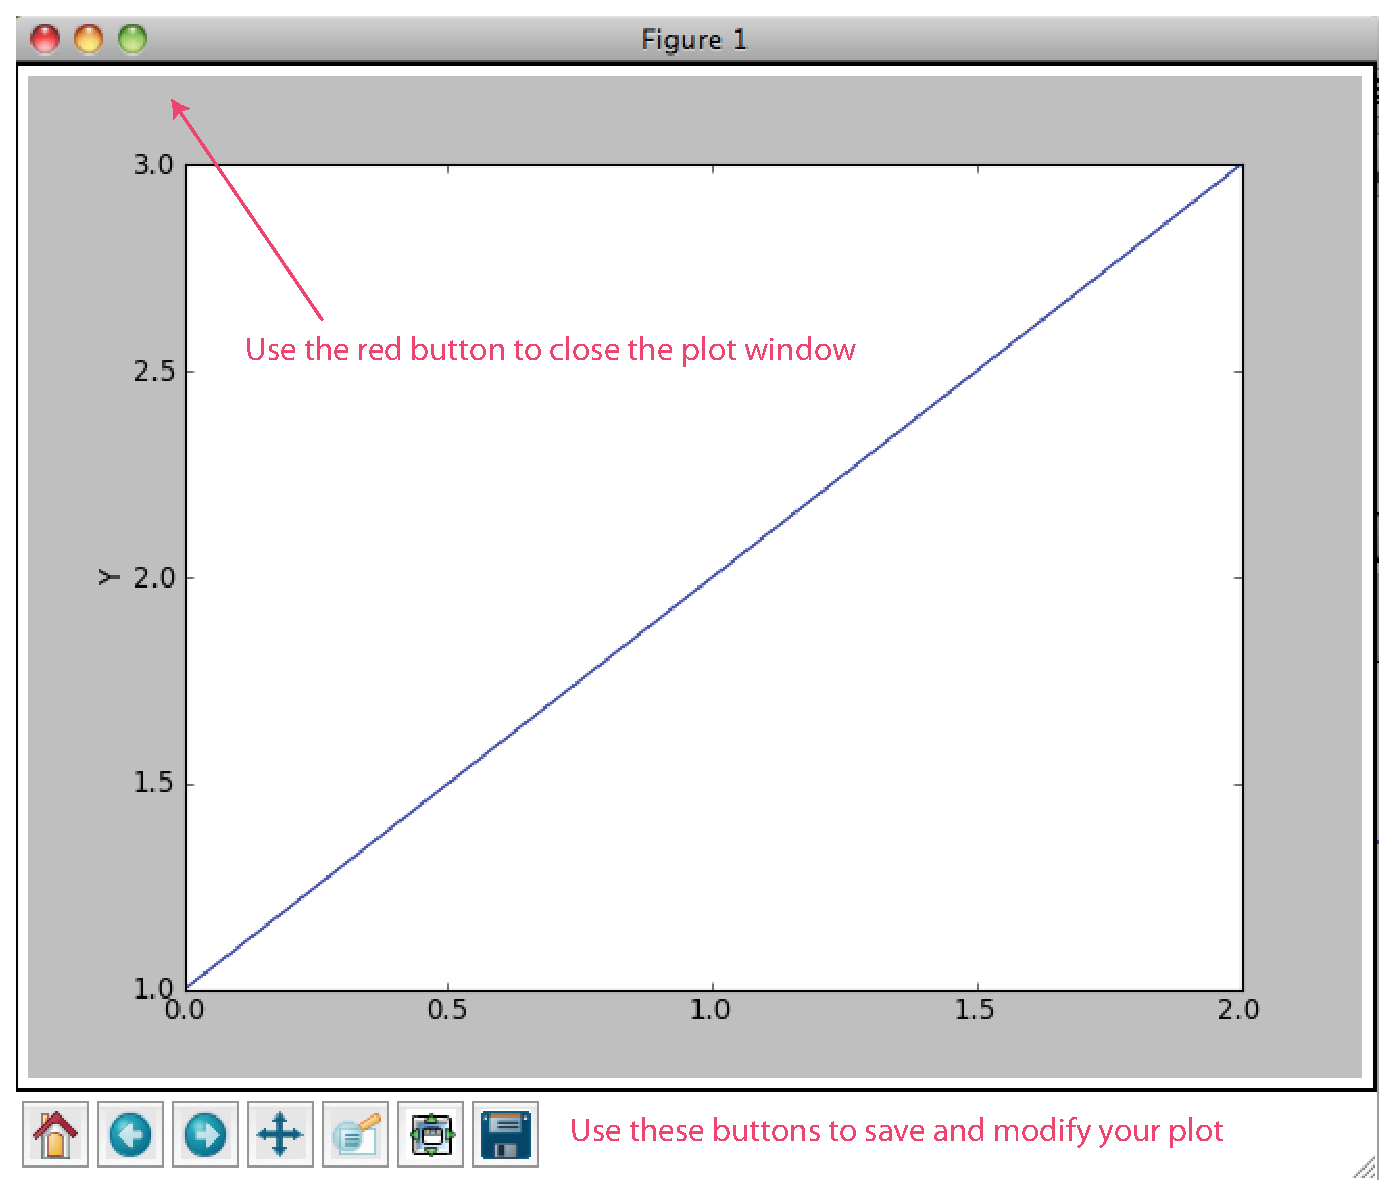
\includegraphics[width=5in]{EPSfiles/matplotlib1.eps} 
   
   \noindent Once that happens, we won't be able to change the plot any more and in fact, we won't get our terminal back until the little plot window is closed.   You can save your plot with the little disk icon in a variety of formats.  Adobe Illustrator likes .svg, or .eps while Microsoft products like .png file formats.  

If you find it annoying to always have to close figures with the little red button, or save them with the disk icon, you can tweak the program like this:

{ \color{blue}\begin{verbatim}
#!/usr/bin/env python
import matplotlib
matplotlib.use("TkAgg") 
import pylab 
pylab.ion()  # turn on interactivity
pylab.plot([1,2,3]) 
pylab.ylabel('Y') 
pylab.draw() # draw  the current plot
ans=raw_input('press [s] to save figure, any other key to quit: ')
if ans=='s':
    pylab.savefig('myfig.eps')
\end{verbatim}}

\noindent The method {\color{blue}pylab.savefig(FILENAME.FMT)}.  The .FMT can be one of several, e.g., .eps, .svg, .ps, .pdf, .png, .gif, .jpg, etc.).   Some of these (the vector graphics ones like pdf,  ps, eps and svg) can be opened in Adobe Illustrator for modification.   


As mentioned earlier, if  you give {\color{blue}plot()} a single sequence of values, it assumes they are $y$ values and supplies the $x$ values for you.  Garbage in, garbage out.  But 
 {\color{blue}plot()} takes an arbitrary number of arguments of the form: ($X_1, Y_1$, line\_style\_1, $X_2, Y_2$, line\_style\_2,  etc.), 
 where 'line\_style' is a string that specifies the line style as illustrated in this script called {\color{blue}matplotlib2.py}


{ \color{blue} \begin{verbatim}
#!/usr/bin/env python
import matplotlib
matplotlib.use("TkAgg")
import pylab,numpy
x=numpy.arange(0,360,10)
r=x*numpy.pi/180.
c=numpy.cos(r)
s=numpy.sin(r)
pylab.plot(x,c,'r--',x,s,'g^')
pylab.show()
\end{verbatim}}

\noindent which produces the plot: 

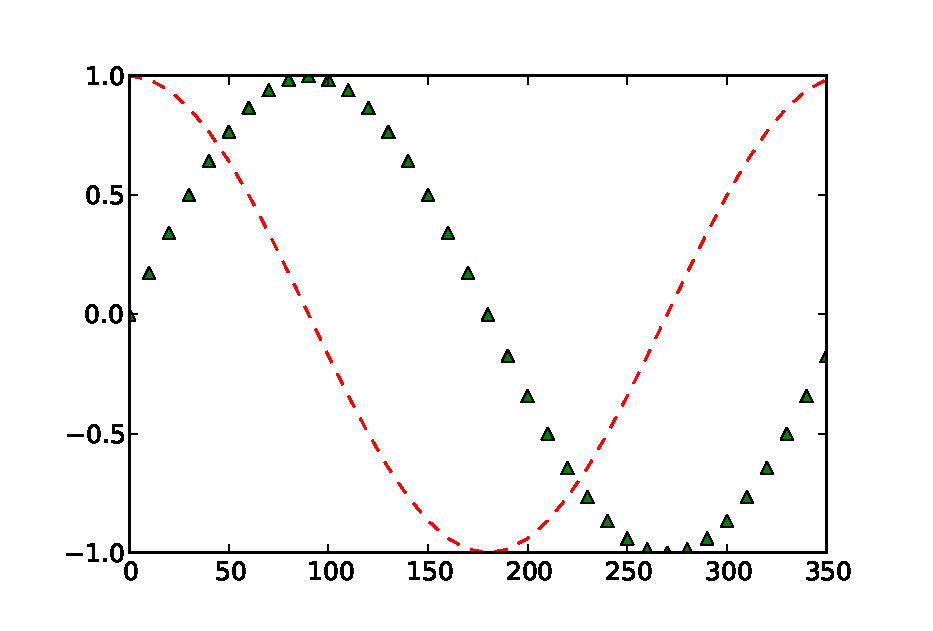
\includegraphics[width=5in]{EPSfiles/matplotlib2.eps}

\noindent   From the code, you can probably figure out that a line style of 'r--' is a red dashed line,  and 'g\verb|^|'  are green triangles.  
There are many other attributes that can be controlled: linewidth, dash style, etc. and I invite you to check out the {\color{blue}matplotlib} documentation.

\noindent By now, you should understand enough about classes, keyword argument passing and other pythonalia to be able to figure things out on your own.   But don't panic, I'm going to lead you through a few more examples, which I hope will speed you on your plotting way.  



\subsection{Multiple figures and more customization}
As already mentioned,  {\color{blue}pylab} has the concept of ``current figure'' which subsequent commands refer to.   In the preceding examples, we only had one figure, so we didn't have to name it, but for fancier figures with several plots, we 
can create  named figure objects by invoking a {\color{blue}figure} instance: 
 
 {\color{blue}\begin{verbatim}
fig = pylab.figure(num=1,figsize=(5,7)). 
\end{verbatim}}

\noindent  Notice the syntax whereby {\color{blue} figsize}  is a method with  width and height (in inches) specified by a tuple and {\color{blue}fignum}  is the figure number.    Notice that these are keyword arguments, and that there are many more:  consult the list of  **kwargs in the online documentation  located here:

 http://matplotlib.sourceforge.net/api/pyplot\_api.html\#matplotlib.pyplot.figure 

Once we have a figure instance (sometimes called a ``container''), we can do all kinds of things, including adding subplots.  To do this, we can use the syntax:

{\color{blue}\begin{verbatim}
 fig.add_subplot(211) 
 \end{verbatim}}
 \noindent Here the 
argument  211 means 2 rows, one column and this is the first plot.  To make plots side by side, you would use: {\color{blue} fig.add\_subplot(121) } for  1 row, two columns, etc.  

After each {\color{blue}add\_subplot} command, that subplot becomes the current figure for plotting on.
If you want more freedom, say, you want to make a subplot at an arbitrary place,  use the {\color{blue}add\_axes([left, bottom,width, height])} 0 method, e.g.,  {{\color{blue}add\_axes([0.1,0.1,0.7,0.3])}.  The values are 0-1 in relative figure coordinates. 

To illustrate these new concepts, consider the example code, {\color{blue}matplotlib3.py}:

{ \color{blue} \begin{verbatim}
#!/usr/bin/env python
import matplotlib
matplotlib.use("TkAgg")
import pylab, numpy
def f(t):
    return numpy.exp(-t)*numpy.cos(2.*numpy.pi*t)
t1= numpy.arange(0.,5.,0.1)
t2= numpy.arange(0.,5.,0.02)
fig=pylab.figure(num=1,figsize=(7,5)) 
fig.add_subplot(211) 
pylab.plot(t1,f(t1),'bo')
pylab.plot(t1,f(t1),'k-') 
fig.add_subplot(212) 
pylab.plot(t2,numpy.cos(2*numpy.pi*t2),'r--')
pylab.xlabel('Time (ms)')
fig.add_axes([.6,.75,.25,.10])
pylab.plot([0,1],[0,1],'r-',[0,1],[1,0],'r-')
pylab.ylabel('Inset')
pylab.show()
\end{verbatim}}

\noindent which produces:

{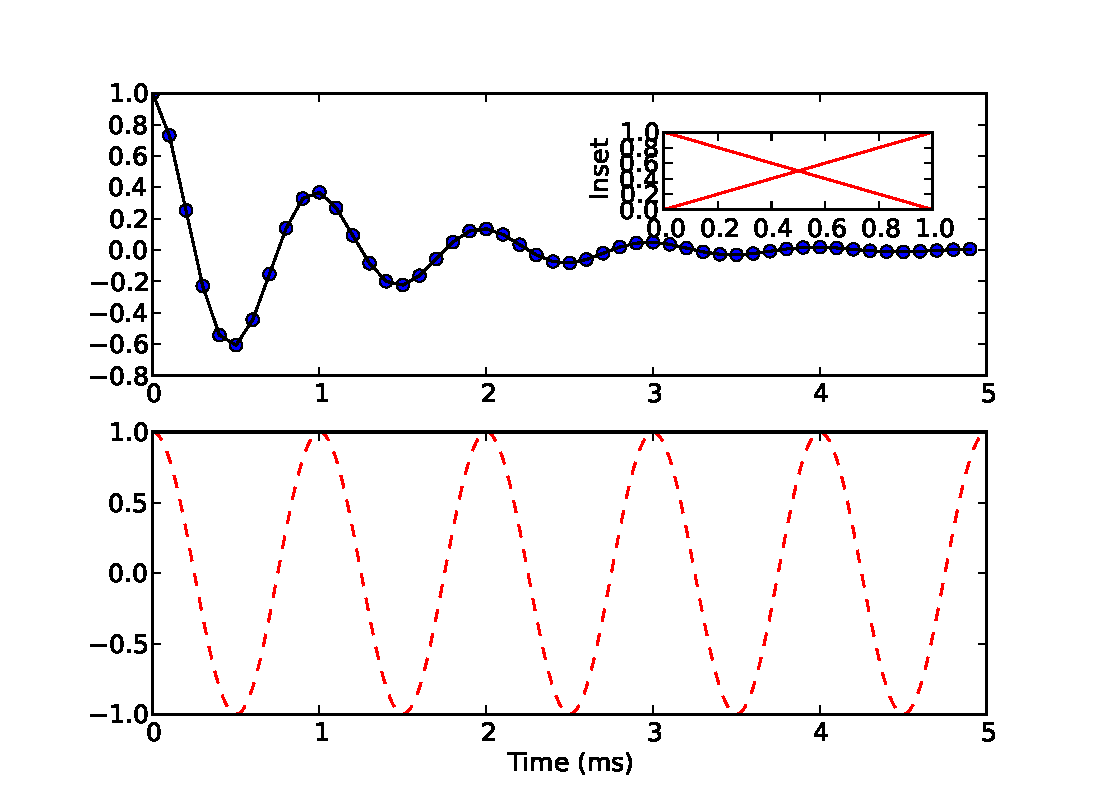
\includegraphics[width=5in]{EPSfiles/matplotlib3.eps}}

\noindent By now, you should be able to figure out what everything in that script does by yourself!  

\subsection{Adding text}

We already met {\color{blue}xlabel} and {{\color{blue}ylabel}.  But text can be added in a other ways, e.g., using the  title, text, legend and arrow methods.
Let's decorate one of our early examples to show how some of these things work:

{ \color{blue} \begin{verbatim}
#!/usr/bin/env python
import matplotlib
matplotlib.use("TkAgg")
import pylab,numpy
x=numpy.arange(0,360,10)
r=x*numpy.pi/180.
c=numpy.cos(r)
s=numpy.sin(r)
s2=numpy.sin(r)**2
pylab.plot(x,c,'r--',x,s,'g^',x,s2,'k-')
pylab.title('Fun with trig')
pylab.text(250,-.5,'pithy note')
pylab.legend(['cos(x)',\
    'sin(x)',r'$\sin(x^2$)'],'lower left')
pylab.xlabel(r'$\theta')
pylab.annotate('triangles!',\
  xy=(175,0),xytext=(110,-.25),\
   arrowprops=dict(facecolor='black',\
   shrink=0.05))
pylab.show()
\end{verbatim}}

\noindent which produces this plot:

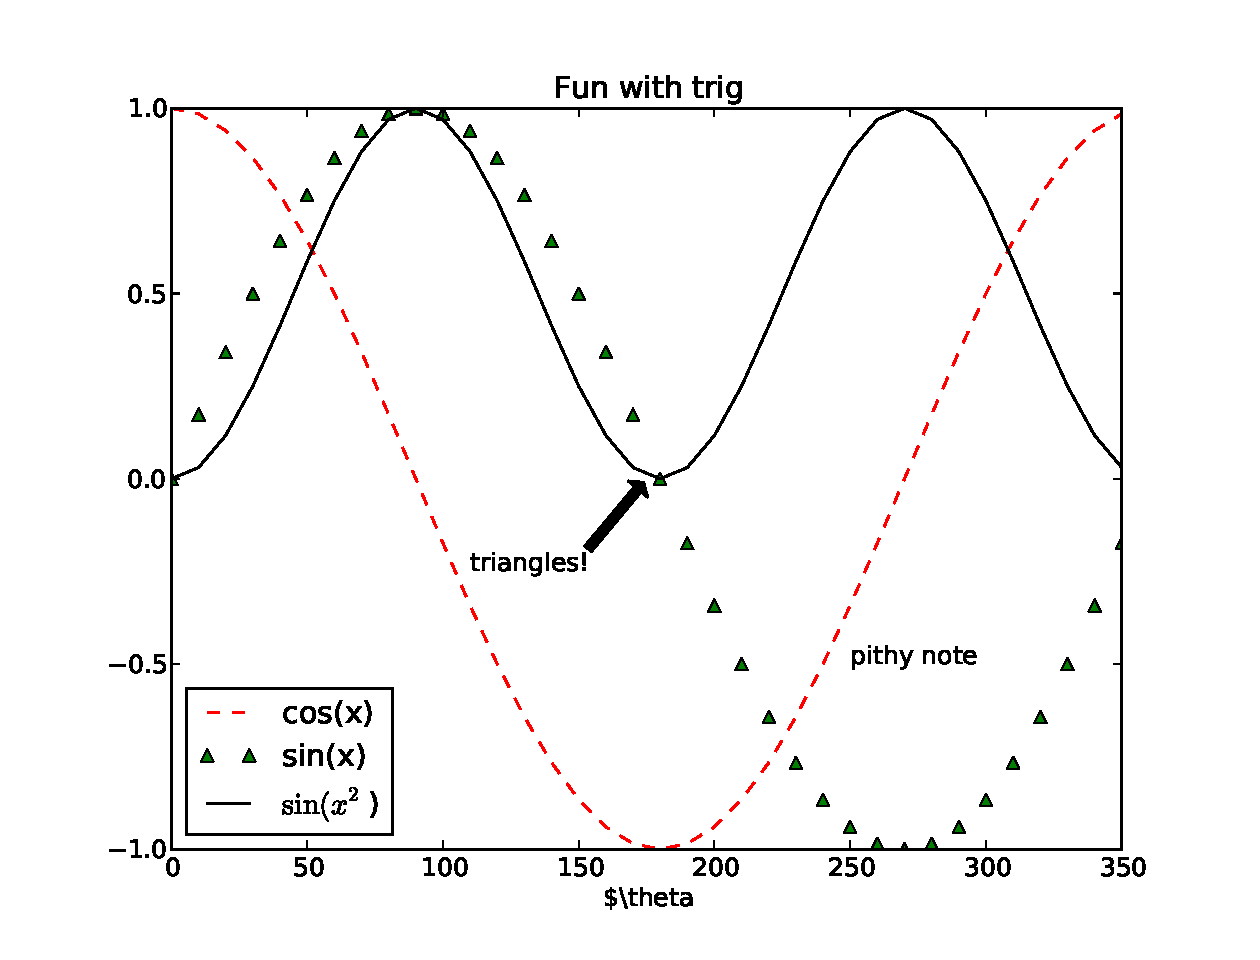
\includegraphics[width=4in]{EPSfiles/matplotlib4.eps}

The title appears at the top of the plot.  
    Text labels get places at the $x$ and $y$ coordinates on the plot and the legend will appear in the upper/lower right/left corner as specified in the string.  The {\color{blue}pylab.text(x,y,string, kwargs)} method also has optional key word arguments, specifying font, size, color and the like.     The legend 'labelist' is a list of labels for each plot element.  So, every line or point style that you want in your legend, append a label to the label list after the relevant plot command. Also note that the legend and xlabel methods use  a special format for strings ({\color{blue}r'LateX String')} which allows embedded LaTeX equation syntax  to make scientific equations look right - so now you have to learn LaTeX!.   Finally, the arrow gets drawn with the {\color{blue}annotate} method, which has a lot of other attributes as well.
Check the {\color{blue}matplotlib} documentation for details.  
    




There are lots of graphing styles possible with {\color{blue}matplotlib}, e.g., histograms, pie charts, contour plots, whisker plots, etc.  I'm just going to show you a few examples.  The best thing to do is to look through the online documentation for a plot that looks like what you need, then modify it.  This is ALWAYS a good approach - start with something that works and fiddle with it until it suits your own particular needs.  



Although there is much much more to do in Python, this documentation is aimed at getting and using {\bf PmagPy}, so let's move on.  



%\customlink{MagIC}
\chapter{The MagIC database and file formats}

A number of the programs in {\bf PmagPy} were  developed to take advantage of the MagIC database and aid getting data in and out of it.   So, we need some basic understanding of what MagIC is and how it is structured.  
MagIC  is an Oracle  database that is part of the EarthRef.org collection of databases and digital reference material.  
Anyone interested in the MagIC database should first become a registered EarthRef.org user.  To do this, go to \url{\http://earthref.org} and click on the {\bf Register} link in the {\bf Topmenu}.   Registration is not required for access to data or browsing around, but is required for uploading of data into the MagIC database, something which we sincerely hope you will have a chance to do.  By registering, you will also be kept informed of our progress through bi-monthly newsletters and other email alerts.    After you register, go to \url{http://earthref.org/MAGIC}.


\section {Perusing the existing data}

The MagIC database is designed to have two web portals, one for paleomagnetic data (PMAG) and one for rock magnetic data (RMAG).  If you click on the PMAG PORTAL link,  you will see a link labeled ``Open the data tab to Start searching'' which, if you click on it, takes you to the main MagIC search engine.  You can look for data from a particular reference by typing in the author's name in the ``Reference Text Search'' box, or search by any column with a little magnifying glass icon.   
  Once the data you want have been identified, you can download the whole data set for example by clicking on the
  icon for the textfile:
  
    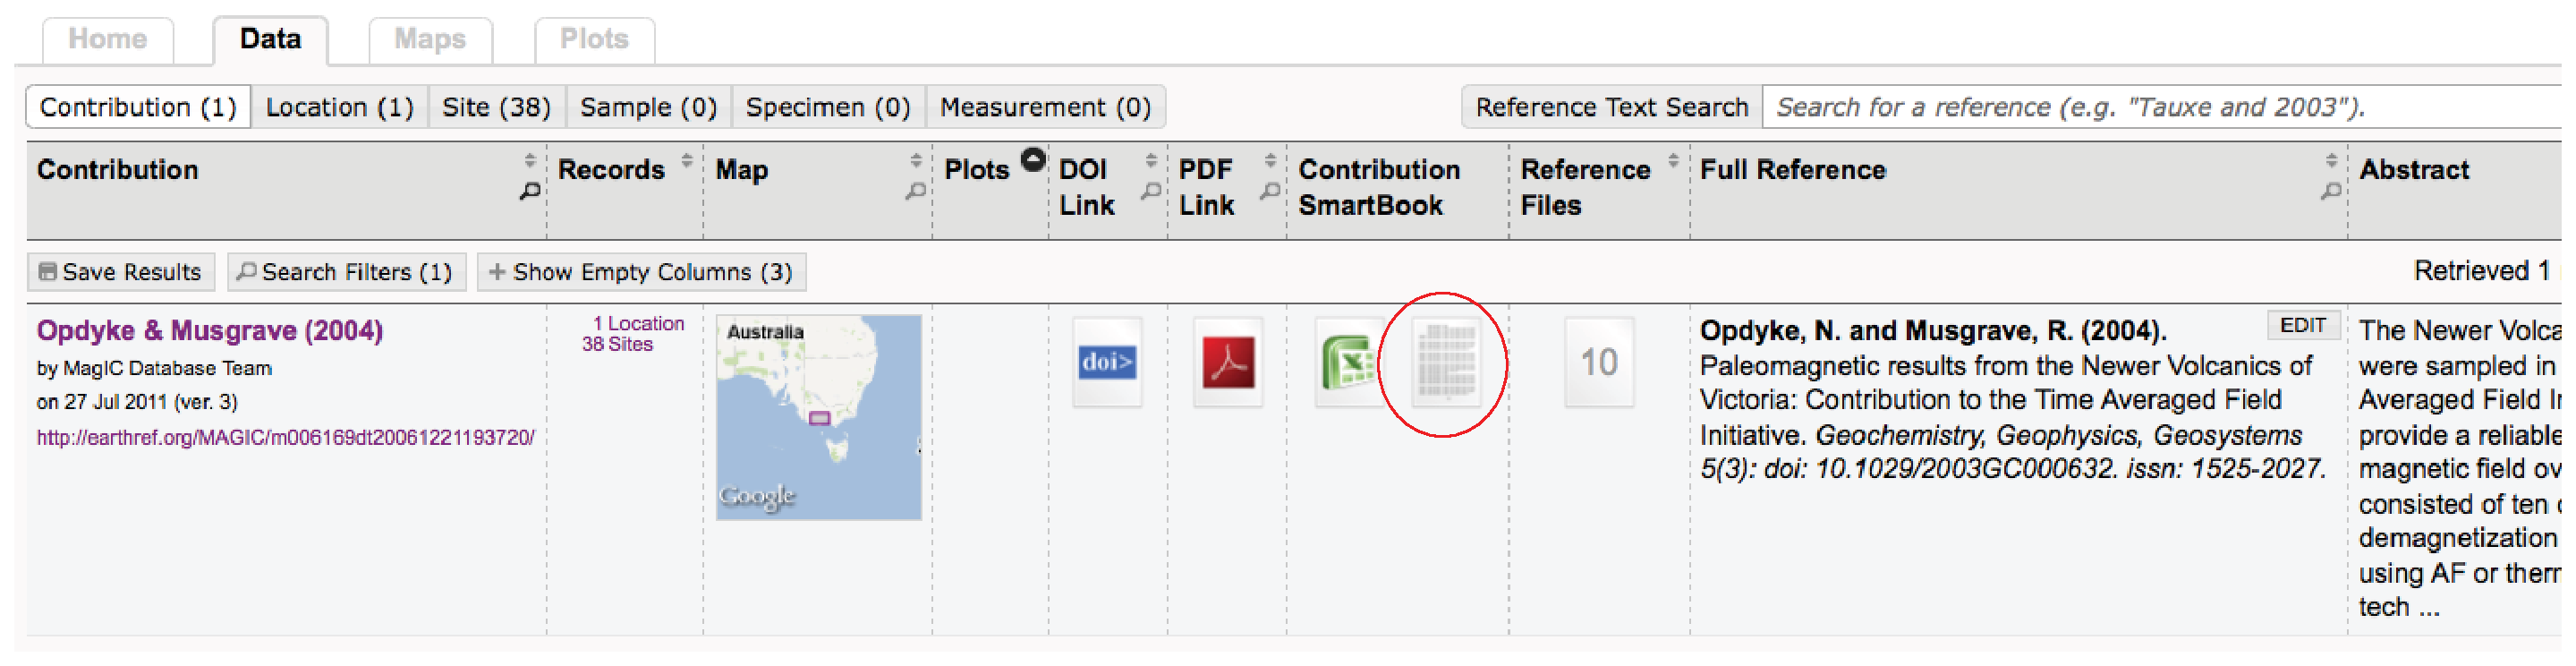
\includegraphics[width=10 in]{EPSfiles/MagIC_search.eps}
  
  
       After downloading, the data can be unpacked and examined using various tools in the {\bf PmagPy}  programs described later.   

\section{Uploading data to the database}

Paleomagnetic and rock magnetic data are collected and analyzed in a wide variety of ways with different objectives.  Data sets can be extremely large or can be the barest boned data summaries published in legacy data tables.   The goal of MagIC has been to have the flexibility to allow a whole range of data including legacy data from publications or other databases to new studies which include all the measurements, field photos, methodology, and so on.  The general procedure for the future will be to archive the data at the same time that they are published.    So, to smooth the path, it is advisable to put your data into the MagIC format as early in the process as possible.  All data that enters the database must pass through    an Excel spreadsheet, called the MagIC Console.  This program allows you to open a ``smartbook''  which comprises some 30 tables each with dozens of column headings (meta-data).      Data are assembled in  a MagIC template file, checked for consistency and completeness, then exported to text and excel files.  These can then be uploaded into the MagIC database.   Data can either be entered directly into the Console, or can be prepared into a strictly formatted ascii file behind the scenes which can be imported into the Console late in the process. In this book we illustrate the use of  a number of programs (the {\bf PmagPy}  package in Python) to facilitate the process.      


\section{Structure of the database tables}  

The MagIC database is organized around a series of data tables.  The complete data model can be found here: 
\url{http://earthref.org/MAGIC/metadata.htm}.   Here is a brief introduction to the data model.  

  Each MagIC table has  a one line header of the form:   

tab\hskip 2em{\bf table\_name}

\noindent
``tab'' (or ``tab delimited'') means that the table is tab delimited.  In theory other delimiters are possible, but {\bf PmagPy}  only  uses tab delimited formats.  The {\bf table\_name} is one of the table names. The tables are of four general types:  EarthRef tables ({\bf er\_}) shared in common with other EarthRef databases,  MagIC tables ({\bf magic\_} tables common to both rock magnetic and paleomagnetic studies, Paleomagnetic tables ({\bf pmag\_}), data reduction useful in paleomagnetic studies, Rock Magnetic tables ({\bf rmag}), data reduction useful for rock magnetic studies.    Most studies use only some of these tables.     Here are some useful tables for a typical paleomagnetic study:

\begin{table}[htb]
\caption{Selected MagIC data tables.}
\label{tab:tables}
\begin{tabular}{ll}
\hline
table&Brief description\\
\hline
{\bf er\_locations}& geographic information about the location(s) of the study\\
 {\bf er\_sites}& locations, lithologic information, etc. for the sampling sites\\
 {\bf er\_samples}& orientation, sampling methods, etc. for samples\\
  {\bf er\_specimens}&specimen weights, volumes\\
    {\bf er\_ages}&Ages information.\\
    {\bf er\_images}& images associated with the study (field shots, sample\\ 
    &photos, photomicrographs, SEM images, etc.\\
   {\bf er\_citations}&citation information\\
   {\bf er\_mailinglist}&contact information for people involved in the study\\
   \hline
   {\bf magic\_measurements}& measurement data used in the study\\
    {\bf magic\_methods}& methods used in the study\\
    {\bf magic\_instruments}& instruments used in the study\\
       \hline
    {\bf pmag\_specimens}& interpretations of best-fit lines, planes, paleointensity, etc. \\
{\bf pmag\_samples}&sample averages of specimen data\\
{\bf pmag\_sites}& Site averages of sample data\\
{\bf pmag\_results}& Averages, VGP/V[A]DM calculations, stability tests, etc.\\
{\bf pmag\_criteria}&criteria used in study for data selection\\
   \hline
   {\bf rmag\_susceptibility}&Experiment for susceptibility parameters\\
{\bf rmag\_anisotropy}& summary of anisotropy parameters\\
{\bf rmag\_hysteresis}& summary of hysteresis parameters\\
{\bf rmag\_remanence}&summary of remanence parameters\\
{\bf rmag\_results}&Summary results and highly derived data \\
&products (critical temperatures, etc.)\\
{\bf rmag\_criteria}&criteria used in study for data selection\\
\hline
\end{tabular}
\end{table}


The second line of every file contains the column headers (meta-data) describing the included data.   For example, a {\bf er\_sites} table might look like this:

{\hoffset -1in
\begin{tabular}{llllll}
\hline
tab\hskip 2em{\bf er\_sites}\\
er\_site\_name&er\_location\_name&site\_lithology&site\_type&site\_lat&site\_lon\\AZ01&Azores&basalt&lava flow&37.80&-25.80\\
...\\
\hline
\end{tabular}
}

Although data can be entered directly into the MagIC Console, it is easier to generate the necessary tables as a by-product of ordinary data processing without having to know details of the meta-data and method codes. 
  The following appendix describes how to use the {\bf PmagPy} software for  data analysis and generate the MagIC data tables automatically for the most common paleomagnetic studies involving directions and/or paleointensities.    
  
  \begin{table}[h]
  \caption{Selected method codes for the MagIC database.}
  \label{tab:meth}
   \begin{tabular}{lll} 
  \hline
  LT-AF-D & Lab Treatment & Alternating field: Double demagnetization\\
  && with AF along X,Y,Z measurement \\
 && followed by AF along -X,-Y,-Z measurement\\
LT-AF-G & Lab Treatment & Alternating field: Triple demagnetization\\ 
&& with AF along Y,Z,X measurement\\
&& followed by AF along Y and AF along Z measurement\\
LT-AF-I & Lab Treatment & Alternating field: In laboratory field\\
LT-AF-Z & Lab Treatment & Alternating field: In zero field\\
LT-CHEM & Lab Treatment & Cleaning of porous rocks by chemical leaching with HCl\\
LT-FC & Lab Treatment & Specimen cooled with laboratory field on\\
LT-HT-I & Lab Treatment & High temperature treatment: In laboratory field\\
LT-HT-Z & Lab Treatment & High temperature treatment: In zero field\\
LT-IRM & Lab Treatment & IRM imparted to specimen prior to measurement\\
LT-LT-I & Lab Treatment & Low temperature treatment: In laboratory field\\
LT-LT-Z & Lab Treatment & Low temperature treatment: In zero field\\
LT-M-I & Lab Treatment & Using microwave radiation: In laboratory field\\
LT-M-Z & Lab Treatment & Using microwave radiation: In zero field\\
LT-NO & Lab Treatment & No treatments applied before measurement\\
LT-NRM-APAR & Lab Treatment & Specimen heating and cooling: Laboratory \\
&&field anti-parallel to the NRM vector\\
LT-NRM-PAR & Lab Treatment & Specimen heating and cooling: Laboratory \\
&&field parallel to the NRM vector\\
LT-NRM-PERP & Lab Treatment & Specimen heating and cooling: \\
&&Laboratory field perpendicular to the NRM vector\\
LT-PTRM-I & Lab Treatment & pTRM tail check: After zero field step, \\
&&perform an in field cooling\\
LT-PTRM-MD & Lab Treatment & pTRM tail check: After in laboratory field step, \\
&&perform a zero field cooling at same temperature\\
LT-PTRM-Z & Lab Treatment & pTRM tail check: After in laboratory field step,\\
&& perform a zero field cooling at a lower temperature\\
LT-T-I & Lab Treatment & Specimen cooling: In laboratory field\\
LT-T-Z & Lab Treatment & Specimen cooling: In zero field\\
LT-VD & Lab Treatment & Viscous demagnetization by applying MU-metal screening\\
LP-X & Lab Treatment & Susceptibility\\
LT-ZF-C & Lab Treatment & Zero field cooled, low temperature IRM imparted\\
LT-ZF-CI & Lab Treatment & Zero field cooled, induced M measured on warming\\
\hline
\end{tabular}
\end{table}

%\customlink{method_codes}
  \section{A word about  method codes}
  
  The MagIC database tags records with ``method codes'' which are short codes that describe various methods associated with a particular data record.  The complete list is available here:  \url{http://earthref.org/MAGIC/methods.htm}.      Most of the time, you do not need to know what these are (there are over a hundred!), but it is helpful to know something about them.  These are divided into several general categories like `geochronology methods' and  'field sampling methods'.   Method codes start with a few letters which designate the category (e.g., GM or FS  for geochronogy and field sampling respectively).   Then there is a second part and possibly also a third part to describe methods with lesser or greater detail.   
The current (version 2.4) method codes that describe various lab treatment methods to give you a flavor for how they work are listed in Table~\ref{tab:meth}.    
  


\chapter{The {\bf PmagPy} software package}
\label{web:pmagpy}

The {\bf PmagPy} software package is a comprehensive set of programs for paleomagnetists and rock magnetists. 
\begin{itemize}
\item    Download and unzip PmagPy package from \url{https://github.com/ltauxe/PmagPy}
\item For initial installation, if you are on a Mac, make a directory in your home directory called {\bf PmagPy} (using the \href{#mkdir}{{\bf mkdir} command)}.  If you are on a PC, make called C:\\PmagPy.
\item Copy ALL the files in your unzipped PmagPy directory into your new {\bf PmagPy} directory, overwriting any previous versions you may have.  
\end{itemize}

When you type something on your command line, your operating system looks for programs of the same name in special places.  These are special ``paths'' so the directory with your Python scripts has to ``be in your path''.  To inform the operating system of the new directory, you need to ``set your path''.    Follow the instructions on the website:
\url{http://magician.ucsd.edu/Software/PmagPy/set_path.html} for your particular system.  


 
 \section{General characteristics of PmagPy programs}
 
{\bf PmagPy}  scripts work by calling them on a \href{#command_line}{command line}.  
 The python scripts must be placed in a directory that is in your ``path''.  To see if this has been properly done, type {\bf dir\_cart.py -h} on the command line and you should get a help message.  If you get a ``command not found'' message, you need to fix your path; check the ``installing python'' page on the software website.   Another possible cause for failure is that somehow, the python scripts are no longer executable.  To fix this, change directories into the directory with the scripts, and type the command:  chmod a+x *.py  

For people who hate command line programs and prefer graphical user interfaces with menus, etc., some of the key programs for interpreting paleomagnetic and rock magnetic data are packaged together in a program called {\bf MagIC.py}.  This can be invoked by typing {\bf MagIC.py} on the command line.  
The {\bf MagIC.py} program generates the desired commands for you, so you do not have to learn UNIX or how to use the command line (except to call the {\bf MagIC.py} program itself).  Nonetheless, some understanding of what is actually happening is helpful, because the {\bf MagIC.py} program is more limited than  full range of {\bf PmagPy} programs.  So, here is a brief introduction to how the {\bf PmagPy} programs work.

  All  {\bf PmagPy} programs print a help message out if you type: {\bf program\_name.py -h} on the command line.  Many have an ``intereactive'' option triggered by typing {\bf program\_name.py -i}.  Many also allow reading from standard input and output.   The help message will explain how each particular program functions.  There are some common features for the command line options: 
  

\begin{enumerate}
\item Switches are from one to three characters long, preceded by a '-'.  
\item The switch '-h' always prints the help message and '-i' allows interactive entry of options. 
\item  Options for command line switches immediately follow the switch.  For example:  -f INPUT -F OUTPUT will set the input file to INPUT and the output to OUTPUT.
\item  The switch for input  files all start with -f and -F for output files.
\item -spc -sam -sit -syn  -loc are switches relating to specimens, samples, sites, synthetics and locations respectively.  
\item Capitalized switches suppress an option (e.g., -A means do not average, while -a means DO average).  
\item -crd [s,g,t] sets the coordinate system 
\item -fmt [svg,png,jpg] the default image format.  
\item -sav  saves the plots silently and quits the program
\end{enumerate}
\newcommand{\stt}{\small\tt}
\newcount\exnum
\outer\def\example{\medbreak\advance\exnum by 1
  \noindent{$\item$ \bf Example \the\exnum\enspace} \noindent}
  
 The {\bf PmagPy} scripts call on two special modules, the {\bf pmag} and the {\bf pmagplotlib} modules.  These contain most of the calculations and plotting functions.  


%\customlink{Examples}
\chapter{Examples of how to use {\bf PmagPy} programs}
\label{ex:PmagPyEx}

In all examples, the '\%' prompt stands for whatever command line prompt you have. 
Download the package containing example data files for this book from: 

{ \url{http://magician.ucsd.edu/Software/PmagPy/Datafiles.zip} }
 
\noindent  and unzip the file.   Data files for the following examples can be found in the {\it Examples} directory.  


%
%\customlink{aarm_magic.py}
\section {\bf aarm\_magic.py}
{ [\href{http://magician.ucsd.edu/Essentials/WebBook2.html#paleomagnetic_tensors}{Chapter 13} 
\href{#MagIC}{[MagIC]}
\label{ex:aarm_magic}
%LJ

Anisotropy of anhysteretic or other remanence can be converted to a tensor and used to correct natural remanence data for the effects of anisotropy remanence acquisition.  For example, directions may be deflected from the geomagnetic field direction or intensities may be biased by strong anisotropies in the magnetic fabric of the specimen.  By imparting an anhysteretic or thermal remanence in many specific orientations, the anisotropy of remanence acquisition can be characterized and used for correction.   We do this for anisotropy of anhysteretic remanence (AARM) by imparting an ARM in 9, 12  or 15 positions.  Each ARM must be preceded by an AF demagnetization step.    The 15 positions are shown in the \href{#k15_magic.py}{k15\_magic.py} example. 




 For the 9 position scheme,  {\bf aarm\_magic.py} assumes that the AARMs are imparted in positions 1,2,3, 6,7,8, 11,12,13.    Someone (a.k.a. Peter Selkin) has kindly made the measurements and saved them an \href{#sio_magic.py}{SIO formatted measurement file} named {\it arm\_magic\_example.dat} in the datafile directory called {\it aarm\_magic}.   Note the special format of these files - the treatment column (column \#2) has the position number (1,2,3,6, etc.) followed by either a ``00'' for the obligatory zero field baseline step or a ``10'' for the in-field step.  These could also be `0` and `1'.    
 
 We need to first import these into the magic\_measurements format and then calculate the anisotropy tensors.  These can then be plotted or used to correct paleointensity or directional data for anisotropy of remanence.  
 
So,  first use the program \href{#sio_magic.py}{\bf sio\_magic.py}  to import the AARM data  into the MagIC format.  The DC field was 50 $\mu$T, the peak AC field was 180 mT, the location was `Bushveld' and the lab protocol was AF and Anisotropy.   The naming convention used Option \# 3 (see help menu). 

Then use the program \href{#aarm_magic.py}{aarm\_magic.py}  to calculate the best-fit tensor and write out the MagIC tables: {\it rmag\_anisotropy} and {\it rmag\_results}.   These files can be used to correct remanence data in a {\it pmag\_specimens} format table (e.g, intensity data) for the effects of remanent anisotropy (e.g., using the program \href{#thellier_magic.py}{thellier\_magic\_redo.py}.

Here is a transcript of a session that works.   Note that the {\bf  sio\_magic.py}  command is all on one line.  

\begin{verbatim}
% sio_magic.py -f arm_magic_example.dat -loc Bushveld -LP AF:ANI -F aarm_measurements.txt 
      -ncn 3 -ac 180 -dc 50 -1 -1

results put in  aarm_measurements.txt


% aarm_magic.py 
Processing:  bg2.01  Number of positions:  9
Processing:  bg2.03  Number of positions:  9
Processing:  bg2.06  Number of positions:  9
......
specimen tensor elements stored in  ./arm_anisotropy.txt
specimen statistics and eigenparameters stored in  ./aarm_results.txt

\end{verbatim}

%\customlink{agm_magic.py}
\section {\bf agm\_magic.py} [\href{http://magician.ucsd.edu/Essentials/WebBook2.html#magnetic_hysteresis}{Chapter 5} \& \href{#MagIC}{[MagIC]}
\label{ex:agm_magic}

%LJ  Lisa - should MagIC link to the magic database, the magic help library, or the appendix in your textbook that has MagIC info?  
%LT Lori - MagIC should link to the database.  FIXED

This program imports Micromag  hysteresis files into magic\_measurements formatted files.   
Because this program imports data into the MagIC database, specimens need also to have sample/site/location information which can be provided on the command line. If this information is not available, for example if this is a synthetic specimen,  specify -syn for synthetic on the command line.    

Someone named Lima Tango has measured a synthetic specimen named {\it myspec}  for hysteresis and saved the data in a file named {\it agm\_example.dat}.   Use the program {\bf agm\_magic.py} to import the data into a magic\_measurements formatted output file.  These were measured using cgs units, so be sure to set the units switch properly.      [These can be plotted using {\bf hysteresis\_magic.py} or {\bf quick\_hyst.py}.]  You can also import IRM acquisition and DC demagnetization curves using {\bf irm\_magic.py}.   {\bf hysteresis\_magic.py} will calculate various hysteresis parameters and put them in the relevant magic tables for you.  ]   
s
\begin{verbatim}
% agm_magic.py -spn myspec -syn -usr "Lima Tango" -f agm_example.dat -u cgs 

results put in  ./agm_measurements.txt

\end{verbatim}

{\bf agm\_magic.py} saved the data in a file called {\it agm\_measurments.txt} which can be combined with other magic\_measurements formatted files using {\bf combine\_magic.py}.    See also how to import irm and backfield data in the help message.  
 
 You can also plot the hysteresis loop with the program {\bf quick\_hyst.py} or {\bf hysteresis\_magic.py}

%
%\customlink{angle.py}
\section {\bf angle.py } [\href{http://magician.ucsd.edu/Essentials/WebBook2.html#QQ2-1-442}{Appendix A.3.4}]
\label{ex:angle}


 Use the program {\bf angle} to calculate the angle ($\alpha$) between two directions $D=350.2, I=26.8; D=98.6, I=67.3$. 

\begin{verbatim}
% angle.py -i
Declination 1: [cntrl-D  to quit] 350.2
Inclination 1: 26.8
Declination 2: 98.6
Inclination 2: 67.3
   72.1 
Declination 1: [cntrl-D  to quit] ^D
Good bye 
\end{verbatim}
 [NB: PC users will get a more angry sounding exit message]
 
 You can also use this program by reading in a filename using the '-f' option or from standard input (with $<$).  Try this out with the test file in the {\it angle} directory ({\it angle.dat}).  First examine the contents of the input file using {\bf head, more}, or {\bf cat}.  The use {\bf angle.py} to calculate the angles.  You can also save your output in a file {\it angle.out} with the '-F' option:
 
 \begin{verbatim}
 % head angle.dat
    11.2    32.9 	    6.4   -42.9 
   11.5    63.7 	   10.5   -55.4 
   11.9    31.4 	  358.1   -71.8 
  349.6    36.2 	  356.3   -45.0 
   60.3    63.5 	   58.9   -56.6 
  351.8    37.6 	   55.0   -45.8 
  345.5    53.1 	   44.8   -26.9 
   12.2    20.1 	   13.6   -54.0 
  352.1    37.6 	    5.1   -39.9 
  341.2    53.8 	   25.1   -61.1 

 % angle.py -f angle.dat
    75.9 
  119.1 
  103.7 
   81.4 
  120.1 
  100.9 
   95.1 
   74.1 
   78.4 
  120.1 
......
.
\end{verbatim}

%\customlink{ani_depthplot.py}
\section {\bf ani\_depthplot.py} 
[\href{http://magician.ucsd.edu/Essentials/WebBook2.html#Paleomagnetic_tensors}{Chapter 13}; 
\href{#MagIC}{[MagIC]}
\label{ex:ani_depth} 

Anisotropy data can be plotted versus depth.  The program {\bf ani\_depthplot.py} uses MagIC formatted data tables of the {\it rmag\_anisotropy.txt} and {\it er\_samples.txt} types.  {\it rmag\_anisotropy.txt} stores the tensor elements and measurement meta-data while {\it er\_samples.txt} stores the depths, location and other information.  Bulk susceptibility measurements can also be plotted if they are available in a {\it magic\_measurements.txt} formatted file.  

In this example, we will use the data from Tauxe et al. (2012) \nocite{tauxe12} measured on samples obtained during Expedition 318 of the International Ocean Drilling Program.  To get the entire dataset, go to the MagIC data base at:  \url{http://earthref.org/MAGIC/}   
and find the data using the search interface.   As a short-cut, you can use the ``permalink'': 

\url{http://earthref.org/MAGIC/m000629dt20120607193954}.   

Download the text file by clicking on the icon under the red arrow in:

  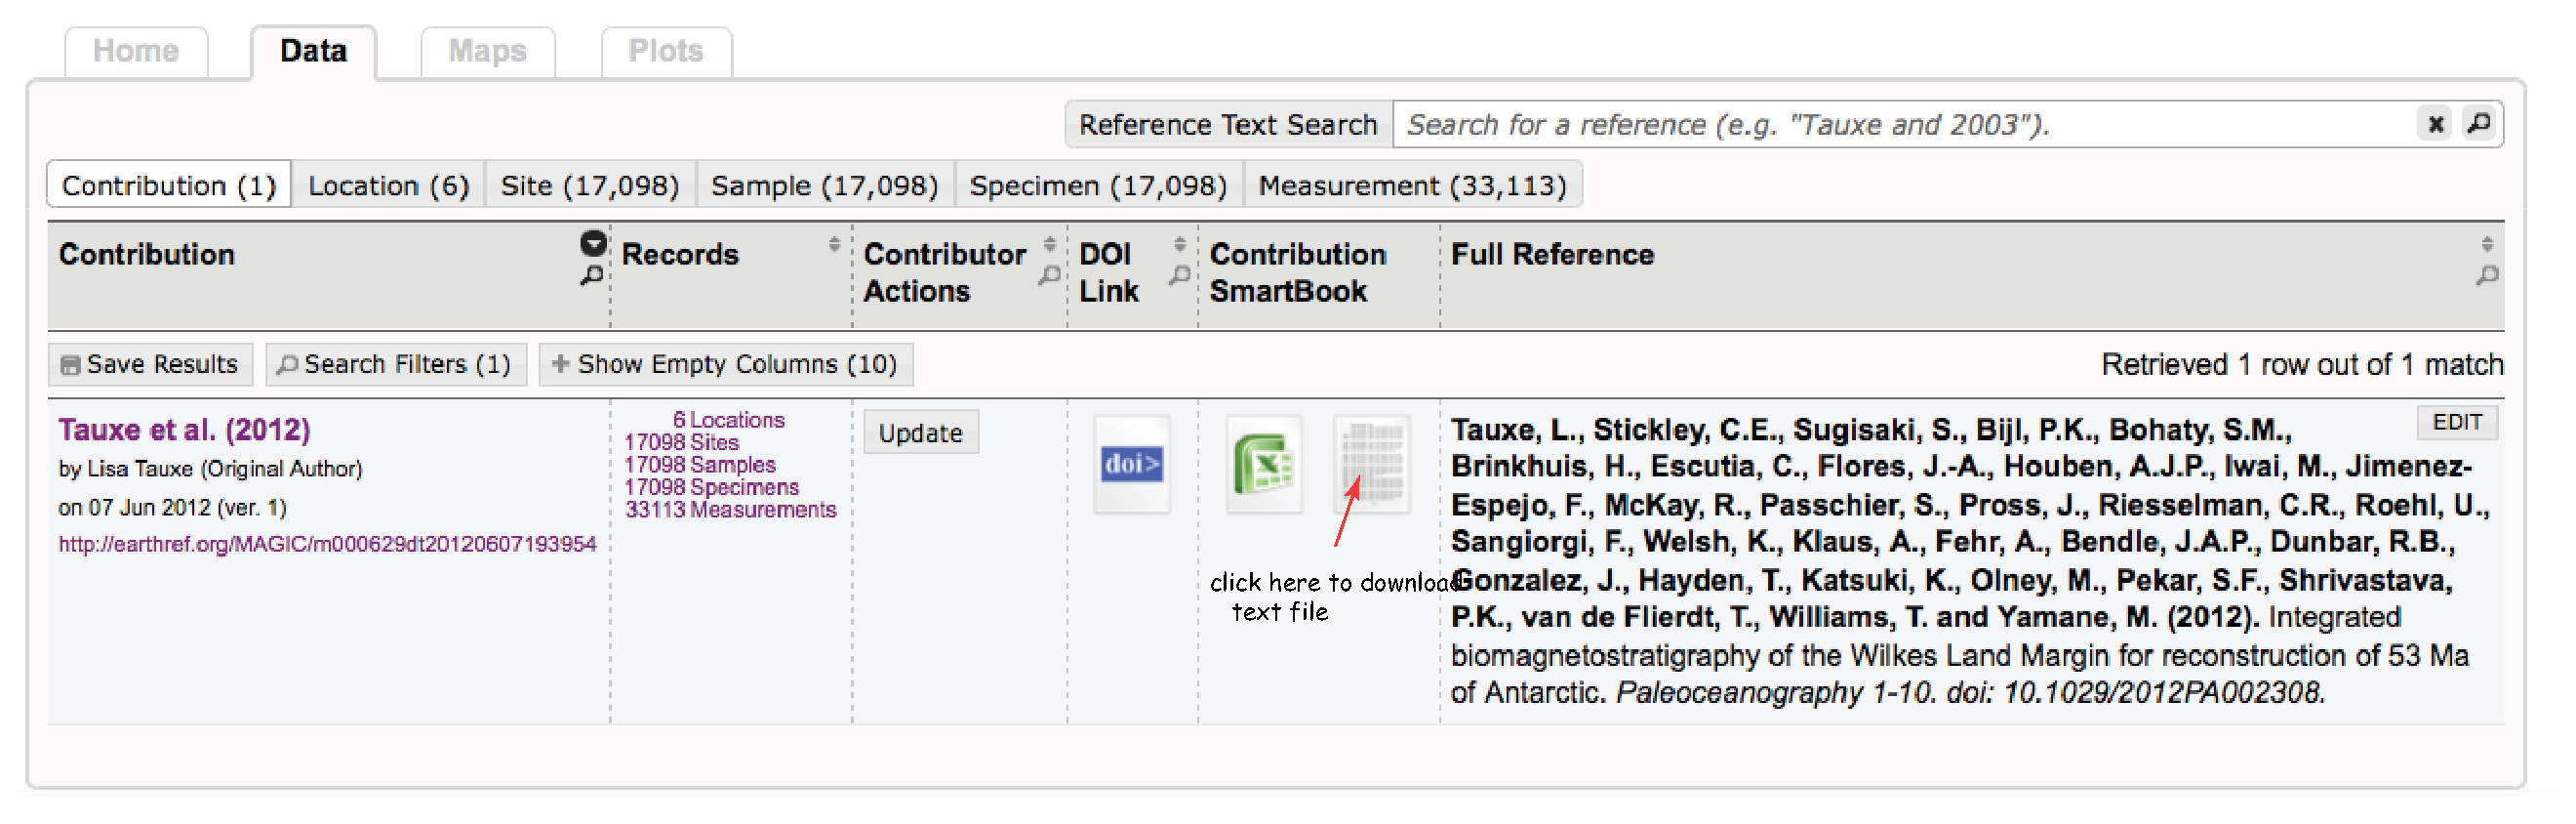
\includegraphics[width=15 cm]{EPSfiles/tauxe12-magic.eps}

Unpack the data using the program in \href{#dowload_magic.py}{download\_magic.py}.  This will unpack the data into the different holes.  Change directories into Location\_2 (which contains the data for Hole U1359A).  Or, you can use the data in the {\bf ani\_depthplot} directory of the \href{#Examples}{example data files}.


\begin{verbatim}
% ani_depthplot.py
\end{verbatim}

\noindent will create the plot:

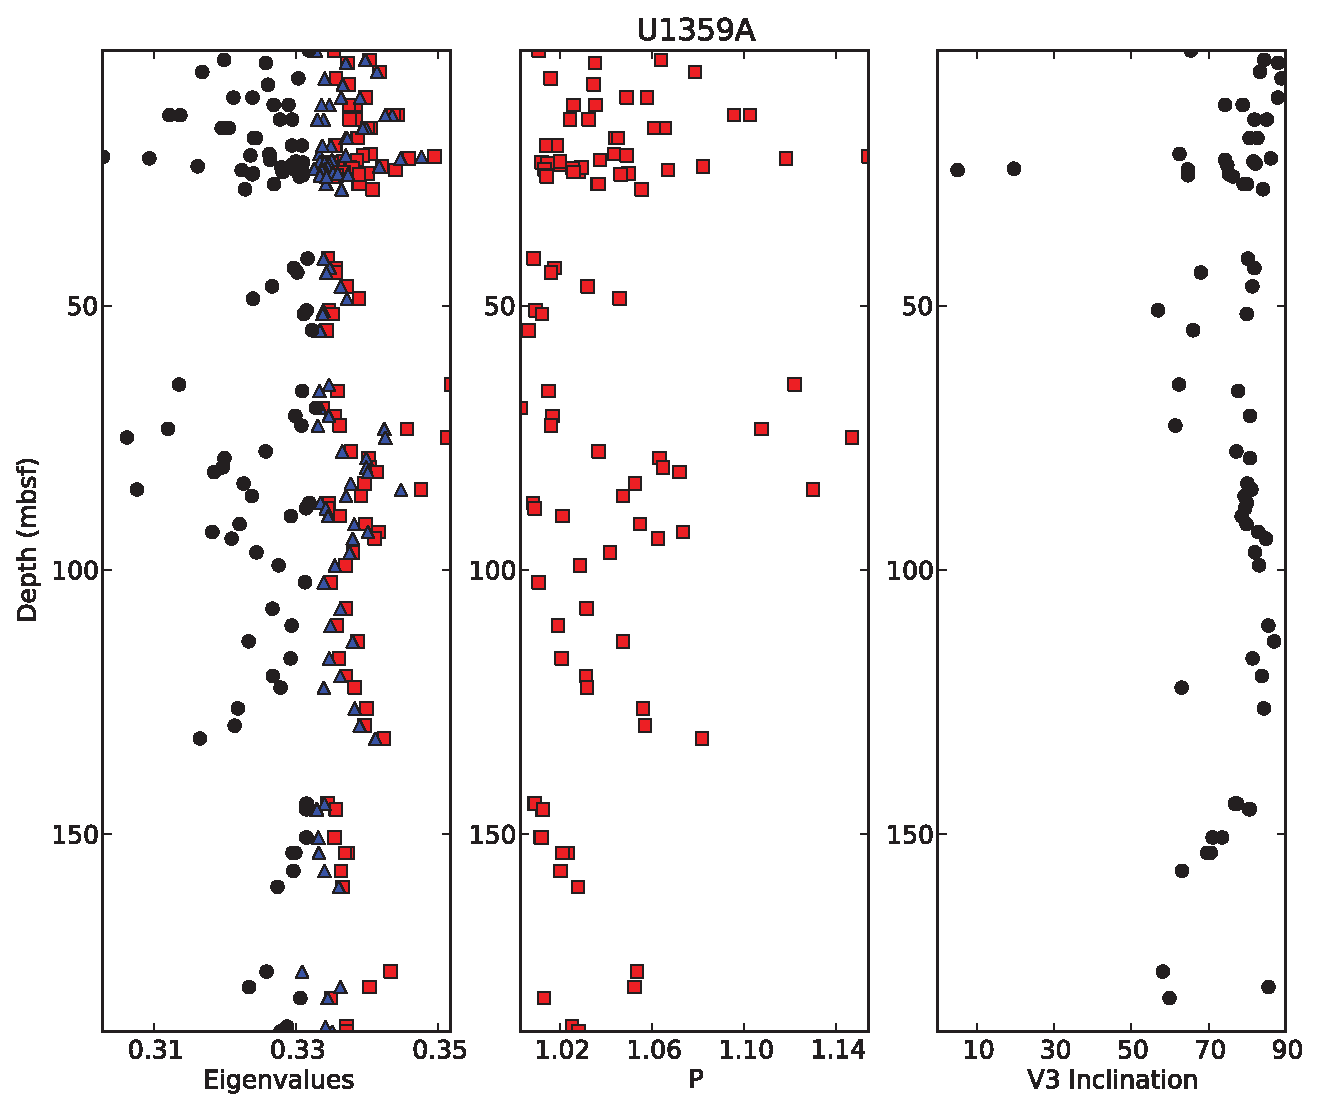
\includegraphics[width=15 cm]{EPSfiles/ani-depthplot.eps}

%\customlink{aniso_magic.py}
\section {\bf aniso\_magic.py} 
[\href{http://magician.ucsd.edu/Essentials/WebBook2.html#Paleomagnetic_tensors}{Chapter 13}; 
\href{#MagIC}{[MagIC]}
\label{ex:aniso_magic} 

Samples were collected from the eastern margin a dike  oriented  with a bedding pole declination of 110$^{\circ}$ and dip of 2$^{\circ}$.      The data have been imported into a rmag\_anisotropy formatted file named {\it dike\_anisotropy.txt}.    

Make a plot of the data using {\bf aniso\_magic.py}.  Use the site parametric bootstrap option and plot out the bootstrapped eigenvectors.   Draw on the trace of the dike.   

These things  are done in this session: 

\begin{verbatim}
% aniso_magic.py -f dike_anisotropy.txt -gtc 110 2 -par -v -crd g
Doing bootstrap - be patient
Boostrap Statistics: 
 tau_i, V_i_D, V_i_I, V_i_zeta, V_i_zeta_D, V_i_zeta_I, V_i_eta, V_i_eta_D, V_i_eta_I
0.34040284    29.6    14.5    26.6    165.5     66.3      6.7    295.5     15.7 
0.33536589   166.3    70.5    24.6     18.7     17.8     11.1    285.7      9.1 
0.32423124   296.2    12.8    12.5    134.6     76.3      6.3     27.3      4.1 
compare with [d]irection 
 plot [g]reat circle,  change [c]oord. system, change [e]llipse calculation,  
     s[a]ve plots, [q]uit 

\end{verbatim}

{\noindent which produced these plots:}

%\epsfxsize 14.5cm

  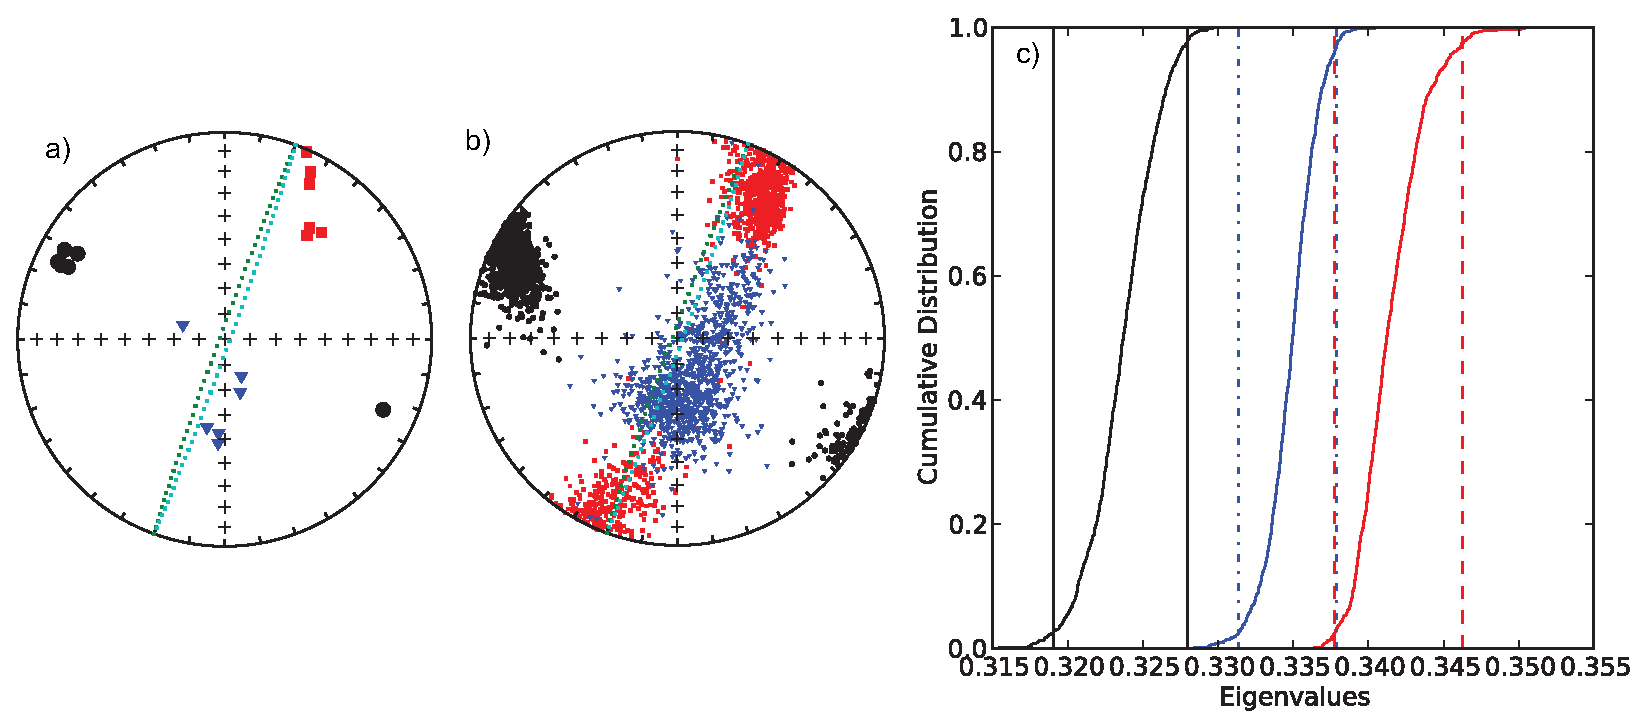
\includegraphics[width=20 cm]{EPSfiles/dike.eps}

The specimen eigenvectors are plotted in the left-hand diagram with the usual convention that squares are the $V_1$ directions, triangles are the $V_2$ directions and circles are the $V_3$ directions.  All directions are plotted on the lower hemisphere.     The bootstrapped eigenvectors are shownin the middle diagramt.   Cumulative distributions of the bootstrapped eigenvalues are shown to the right with the 95\% confidence bounds plotted as vertical lines.  
It appears that the magma was moving in the northern and slightly up direction along the dike.  

There are more options to {\bf aniso\_magic.py} that come in handy.   In particular, one often wishes to test if a particular fabric is isotropic (the three eigenvalues cannot be distinguished), or if a particular eigenvector is parallel to some direction. For example, undisturbed sedimentary fabrics are oblate (the maximum and intermediate directions cannot be distinguished from one another, but are distinct from the minimum) and the eigenvector associated with the minimum eigenvalue is vertical. These criteria can be tested using the distributions of bootstrapped eigenvalues and eigenvectors.   

The following session illustrates how this is done, using the data in the test file {\it sed\_anisotropy.txt} in the aniso\_magic directory.

\begin{verbatim}
%aniso_magic.py -f sed_anisotropy.txt -d 3 0 90 -v -crd g

Doing bootstrap - be patient
Boostrap Statistics: 
 tau_i, V_i_D, V_i_I, V_i_zeta, V_i_zeta_D, V_i_zeta_I, V_i_eta, V_i_eta_D, V_i_eta_I
0.33673459   359.5     7.9     3.1    157.5     81.5      9.2    269.1      3.2 
0.33546969    89.5     0.0  1349.7    303.3     55.0    153.4    179.7     21.2 
0.32779574   179.6    82.1     3.2    358.7      7.9      4.2     88.7      0.1 
compare with [d]irection 
 plot [g]reat circle,  change [c]oord. system, change [e]llipse calculation,  
      s[a]ve plots, [q]uit 
 \end{verbatim}
 
 which makes these plots:
 
   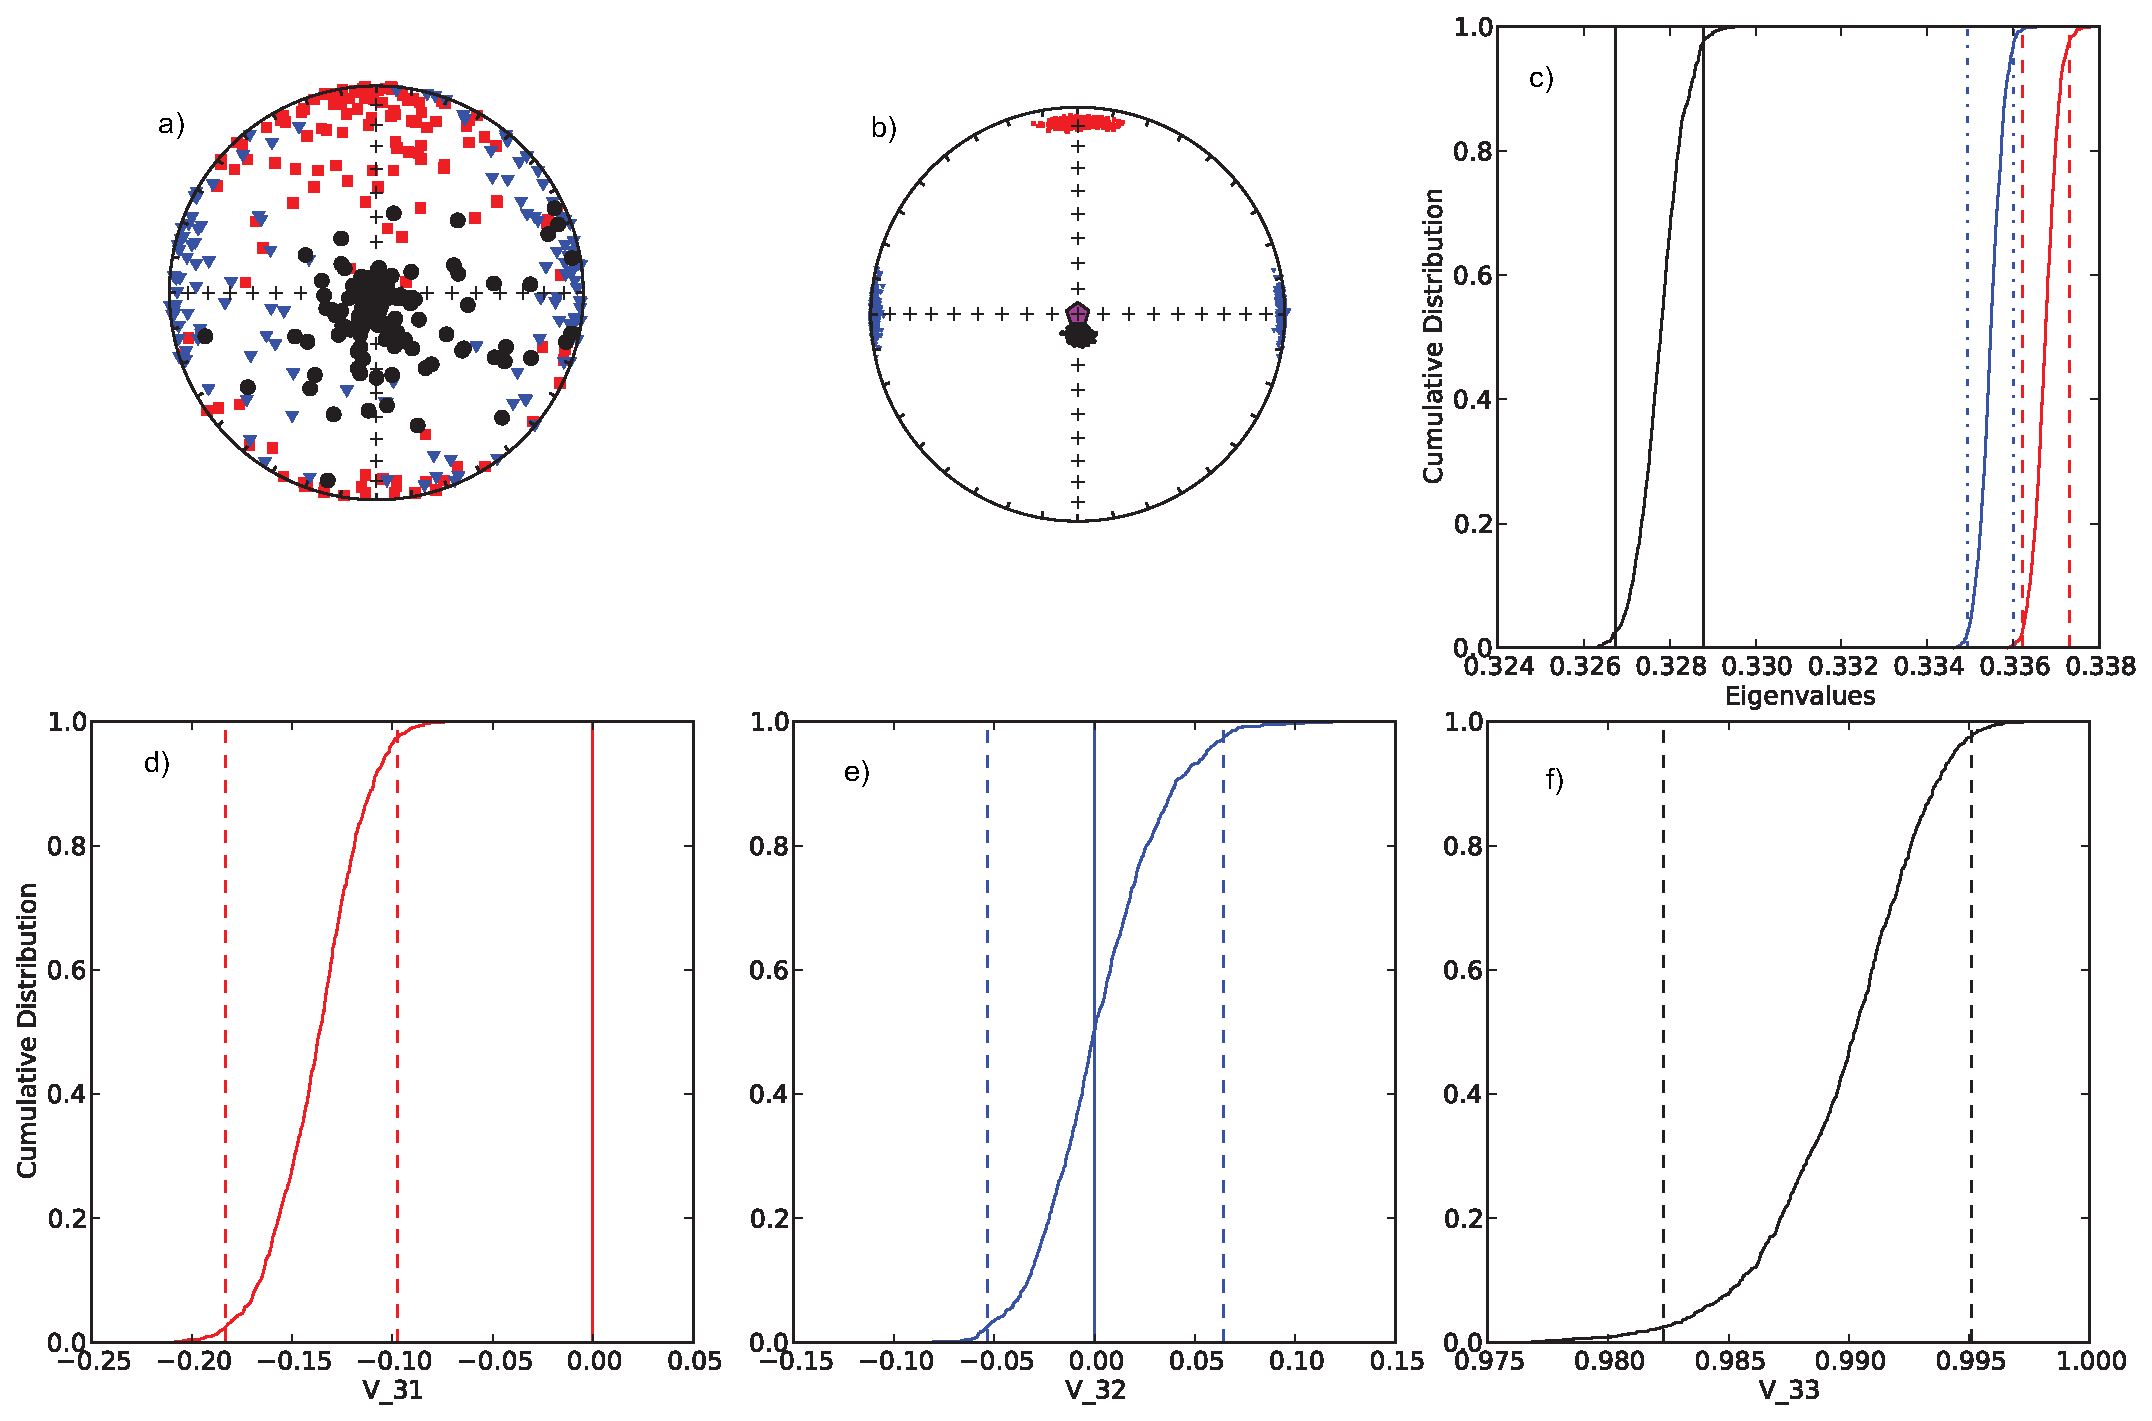
\includegraphics[width=20 cm]{EPSfiles/sed-aniso.eps}
   
   The top three plots are as in the dike example before, showing a clear triaxial fabric (all three eigenvalues and associated eigenvectors are distinct from one another.  In the lower three plots we have the distributions of the three components of the chosen axis,  $V_3$, their 95\% confidence bounds (dash lines) and the components of the designated direction (solid line).  This direction is also shown in the equal area projection above as a red pentagon.  The minimum eigenvector is not vertical in this case.    
 


%\customlink{apwp.py}
\section {\bf apwp.py }
\href{http://magician.ucsd.edu/Essentials/Webbookcopy.html#Tectonic_applications_of_paleomagnetism}{[Chapter 16]}
\label{apwp}

The program {\bf apwp.py} calculates paleolatitude, declination, inclination from  a pole latitude and longitude based on  the paper Besse and Courtillot (2002; see  \href{http://magician.ucsd.edu/Essentials/Webbookcopy.html#x1-19500016}{Chapter 16} for reference and complete discussion).  
Use it  to calculate the expected direction for 100 million year old rocks at a locality in La Jolla Cove (Latitude: 33N, Longitude 117W).    Assume that we are on the North American Plate!  (Note that there IS no option for the Pacific plate in the program {\bf apwp.py}, and that La Jolla was on the North American plate until a few million years ago (6?).   

\begin{verbatim}
% apwp.py -i

 Welcome to paleolatitude calculator - CTRL-D to quit

pick a plate: NA, SA, AF, IN, EU, AU, ANT, GL 

Plate
NA
Site latitude
33
 Site longitude
-117
 Age
100
Age  Paleolat.  Dec.  Inc.  Pole_lat.  Pole_Long.
   100.0    38.8   352.4    58.1    81.5   198.3

\end{verbatim}

Note that as with many {\bf PmagPy}  programs, the input information can be read from a file and the output can be put in a file.   For example, we put the same information into a file, {\it apwp\_example.dat} and use this syntax:

\begin{verbatim}
% apwp.py -f apwp_example.dat
   100.0    38.8   352.4    58.1    81.5   198.3
\end{verbatim}

%\customlink{atrm_magic.py}
\section {\bf atrm\_magic.py}
{ [\href{http://magician.ucsd.edu/Essentials/WebBook2.html#Paleomagnetic_tensors}{Chapter 13} 
\href{#MagIC}{[MagIC]}
\label{ex:atrm_magic}

Anisotropy of thermal  remanence (ATRM) is similar to anisotropy of anhysteretic remanence (AARM) and the procedure for obtaining the tensor is also similar.  Therefore, the program {\bf atrm\_magic.py} is quite similar to \href{#aarm_magic.py}{aarm\_magic.py}.  However, the SIO lab procedures for the two experiments are somewhat different.  In the ATRM experiment, there is a single, zero field step at the chosen temperature which is used as a baseline.  We use only six positions (as opposed to nine for AARM) because of the additional risk of alteration at each temperature step.  The positions are also different:  

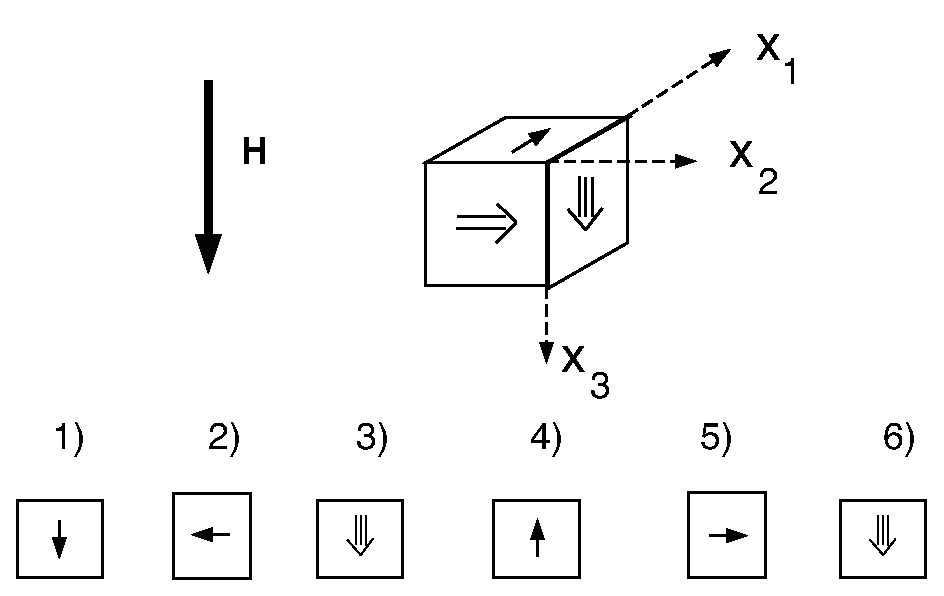
\includegraphics[width=12 cm]{EPSfiles/atrm_meas.eps}

The file {\it atrm\_magic\_example.dat} in the {\it atrm\_magic} directory is an SIO formatred data file containing ATRM measurement data done in a temperature of 520$^{\circ}$C.   Note the special format of these files - the treatment column (column \#2) has the temperature in centigrade followed by either a ``00'' for the obligatory zero field baseline step or a ``10'' for the first postion, and so on.  These could also be `0` and `1', etc..    
 
Use the program \href{#sio_magic.py}{sio\_magic.py} to import the ATRM data  into the MagIC format.  The DC field was 40 $\mu$T.  The naming convention used option \# 1 (see help menu). 
Then use the program {\bf atrm\_magic.py} to calculate the best-fit tensor and write out the MagIC tables: {\it rmag\_anisotropy} and {\it rmag\_results} formatted files.   These files can be used to correct remanence data in a {\it pmag\_specimens} format table (e.g, intensity data) for the effects of remanent anisotropy (e.g., using the program \href{#thellier_magic.py}{thellier\_magic\_redo.py}.

Here is an example transcript:

\begin{verbatim}
% sio_magic.py -f atrm_magic_example.dat -loc Africa -LP T:ANI -F atrm_measurements.txt 
      -ncn 1  -dc 40 -1 -1

results put in  atrm_measurements.txt


% atrm_magic.py 
Processing:  ak01a
Processing:  ak01b
Processing:  ak01c
......
specimen tensor elements stored in  ./trm_anisotropy.txt
specimen statistics and eigenparameters stored in  ./atrm_results.txt
\end{verbatim}

%\customlink{azdip_magic.py}
\section {azdip\_magic.py}
 [\href{http://Webbookcopy.html#Getting_Direction}{Chapter 9} and \href{#MagIC}{[MagIC]}% NOTE: MAKE THIS LINK SPECIFIC TO HELP PAGES FOR ORIENTATION CONVENTIONS

Many paleomagnetists save orientation information in files in this format:

\begin{tabular}{lllll}
Sample & Azimuth & Plunge & Strike & Dip\\
\end{tabular}
\noindent where the Azimuth and Plunge are the declination and inclination of the drill direction and the strike and dip are the attitude of the sampled unit (with dip to the right of strike).   The MagIC database convention is to 
use the direction of the $X$ coordinate of the specimen measurement system.  To convert an  {\it AzDip} formatted file ({\it example.az}) for samples taken from a location name ``Northern Iceland''  into the MagIC format and save the information in the MagIC {\it er\_samples.txt}  file format, use the program {\bf azdip\_magic.py}:

\begin{verbatim}
% azdip_magic.py -f azdip_magic_example.dat -ncn 1 -mcd FS-FD:SO-POM
      -loc "Northern Iceland"

Data saved in  er_samples.txt
\end{verbatim}

Note that there are many options for relating sample names to site names and we used the first convention that has a single character at the end of the site name to designate each sample (e.g., is132d is sample 'd' from site is132).   We have also specified certain field sampling and orientation method codes (-mcd), here field sampling-field drilled (FS-FD) and sample orientation-Pomeroy (SO-POM).  The location was ``Northern Iceland''.   See the help menu for more options.   

Another way to do this is to use the \href{#orientation_magic.py}{orientation\_magic.py} program which allows much more information to be imported.  

%\customlink{b_vdm.py}
\section {\bf b\_vdm.py} 
\href{http://Webbookcopy.html#The_geomagnetic_field}{[Chapter 2]}
\label{ex:b_vdm}

Use the program {\bf b\_vdm} to convert an estimated paleofield value of 33 $\mu$T obtained from a lava flow at 22$^{\circ}$ N latitude to the equivalent Virtual Dipole Moment (VDM) in Am$^2$.   Put the input information into a file called {\it vdm\_input.dat}  and read from it using standard input:

\begin{verbatim}
% cat > b_vdm_example.dat
33 22
^D
% b_vdm.py < b_vdm_example.dat
 7.159e+22 
\end{verbatim}

%\customlink{basemap_magic.py}
\section{basemap\_magic.py}
\label{ex:basemap_magic}
\href{#MagIC}{[MagIC]}

Python has a complete map plotting package and PmagPy has a utility for making simple base maps for projects.  Site location data imported for example using \href{#orientation_magic.py}{orientation\_magic.py} into an {\it er\_sites} formatted text file can be plotted using {\bf basemap\_magic.py}.  There are many options, so check the help message for more details.   Note that if you want to use high resolution, you must install the high resolution continental outlines as described on the  \href{http://magician.ucsd.edu/software/pmagpy/}{PmagPy} website.

As an example, use the program {\bf basemap\_magic.py} to make  a simple basemap plot with site locations in a MagIC {\it er\_sites.txt}  formatted file named {\it basemap\_example.txt}.  

\begin{verbatim}
% basemap_magic.py -f basemap_example.txt 
\end{verbatim}

\noindent which makes this plot:



%\epsfxsize 9cm

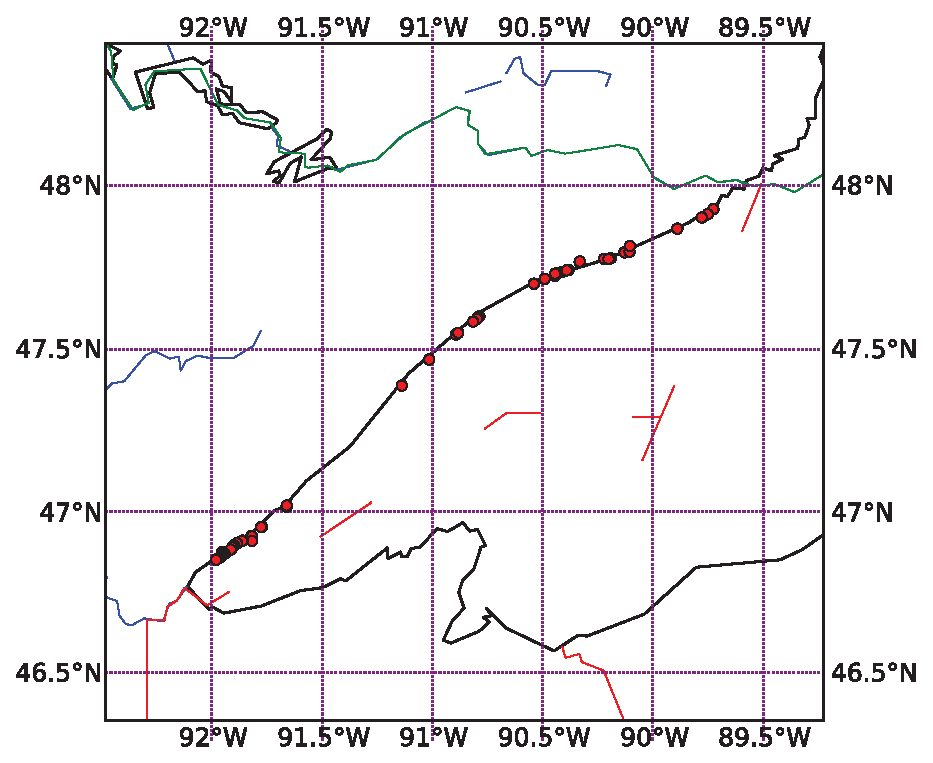
\includegraphics[width= 15 cm]{EPSfiles/basemap.eps}

  Use the buttons at the bottom of the plot to resize or save the plot in the desired format.  


%\customlink{biplot_magic.py}
\section {\bf biplot\_magic.py} 
\label{ex:biplot_magic}
\href{http://Webbookcopy.html#Applied_rock_magnetism}{
[Chapter 8]} and \href{#MagIC}{[MagIC]}

It is often useful to plot measurements from one experiement against another.  For example, rock magnetic studies of sediments often plot the IRM against the ARM or magnetic susceptibility.  All of these types of measurements can be imported into a single {\it magic\_measurements} formatted file, using magic method codes and other clues (lab fields, etc.) to differentiate one from another.  
Data  were obtained from a Paleogene core from 28$^{\circ}$S for a relative paleointensity study.    IRM, ARM, magnetic susceptibility and remanence data were uploaded to the MagIC database.  The magic\_measurements formatted file for this study is saved in {\it core\_measurements.txt}.  

Use the program {\bf biplot\_magic.py} to make a biplot of  magnetic susceptibility against ARM.  Note that the program makes use of the \href{#method_codes}{MagIC method codes} which are LT-IRM for IRM, LT-AF-I for ARM (AF demagnetization, in a field), and LP-X for magnetic susceptibility.  

First, to find out which data are available, run the program like this: 

\begin{verbatim}
% biplot_magic.py -f biplot_magic_example.txt
   which responds with this:
   ['LT-AF-Z', 'LT-AF-I', 'LT-IRM', 'LP-X']
   \end{verbatim}

These are the method codes for  AF demagnetization of NRM, ARM, IRM and susceptibility measurements respectively.  So to make a plot of 
susceptibility against ARM, we would run the program again:


\begin{verbatim}
% biplot_magic.py -f biplot_magic_example.txt -x LP-X -y LT-AF-I
LP-X  selected for X axis
LT-AF-I  selected for Y axis
All
measurement_magn_mass  being used for plotting Y
measurement_chi_mass  being used for plotting X.

S[a]ve plots, [q]uit,  Return for next plot 
\end{verbatim}

\noindent which makes the plot:

%\epsfxsize 10cm
{\hskip 1in %\epsffile{EPSfiles/arm-x.eps}
  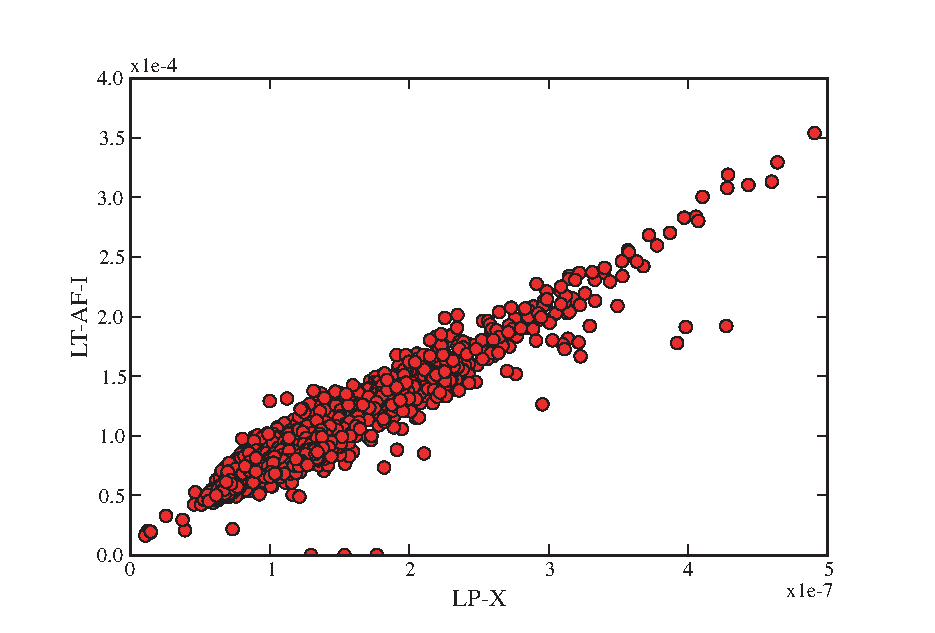
\includegraphics[width=15 cm]{EPSfiles/arm-x.eps}}
  
  
%\customlink{bootams.py}
\section {\bf bootams.py} 
\href{http://magician.ucsd.edu/Essentials/WebBook2.html#Paleomagnetic_tensors}{Chapter 13}
\label{ex:bootams}

The program {\bf bootams.py} calculates bootstrap statistics for anisotropy tensor data in the form of:

x11 x22 x33 x12 x23 x13

It does this by selecting para-data sets and calculating the Hext average eigenparameters.   
It has an optional parametric bootstrap whereby the $\sigma$ for the data set as a whole is used to draw new para data sets.    The bootstrapped eigenparameters are assumed to be Kent distributed and the program calculates Kent error ellipses for each set of eigenvectors.  It also estimates  the standard deviations of the bootstrapped eigenvalues.   

Use this to calculate the bootstrapped error statistics for the data in file {\it  bootstrap\_examples.data}:

\begin{verbatim}
% bootams.py -par -f bootams_example.dat
Doing bootstrap - be patient

tau tau_sigma V_dec V_inc V_eta V_eta_dec V_eta_inc V_zeta V_zeta_dec V_zeta_inc

0.33505 0.00040     5.3    14.7    32.5   267.1    25.7    89.2   141.7    50.2
0.33334 0.00041   124.5    61.7    40.2    29.8     2.2    46.6   298.9    23.6
0.33161 0.00047   268.8    23.6    26.7     6.0    14.8    57.6   119.1    56.0

\end{verbatim}

%
%\customlink{cart_dir.py}
\section {cart\_dir.py}
\href{http://magician.ucsd.edu/Essentials/WebBook2.html#The_geomagnetic_field}{[Chapter 2]} 
\label{ex:cart_dir}

Use the program {\bf cart\_dir} to convert these cartesian
coordinates to geomagnetic elements:


\begin{tabular}{ccc}
\hline
 $x_1$ & $x_2$ & $x_3$\cr
\hline
   0.3971 &  -0.1445  &  0.9063\cr
  -0.5722 &    0.0400  & -0.8192\cr
\hline
\end{tabular}


To use the interactive option:

\begin{verbatim}
% cart_dir.py -i
X: [cntrl-D  to quit] 0.3971
Y: -0.1445
Z: 0.9063
  340.0    65.0  1.000e+00
X: [cntrl-D  to quit] -.5722
Y: 0.0400
Z: -0.8192
  176.0   -55.0  1.000e+00
\end{verbatim}

To read from a file:

\begin{verbatim}
% cart_dir.py -f cart_dir_example.dat
  340.0    65.0  1.000e+00
  176.0   -55.0  1.000e+00
\end{verbatim} 

%\customlink{chartmaker.py}
\section{chartmaker.py}
\label{ex:chartmaker}
\href{http://magician.ucsd.edu/Essentials/WebBook2.html#Paleointensity}{[Chapter 10]}

Paleointensity experiments are quite complex and it is easy to make a mistake in the laboratory.  The SIO lab uses a simple chart that helps the experimenter keep track of in-field and zero field steps and makes sure that the field gets verified before each run.   You can make a chart for an infield-zerofield, zerofield-infield (IZZI) experiment using the program {\bf chartmaker.py}.   Make such a chart using 50$^{\circ}$C steps up to 500$^{\circ}$C  followed by 10$^{\circ}$C steps up to 600$^{\circ}$C.

\begin{verbatim}
% chartmaker.py
    Welcome to the thellier-thellier experiment automatic chart maker.   
    Please select desired step interval and upper bound for which it is valid.
    e.g.,   
    50 
    500
    10 
    600
    
    a blank entry signals the end of data entry.
    which would generate steps with 50 degree intervals up to 500, followed by 10 degree intervals up to 600.   
    
    chart is stored in:  chart.txt
    
 Enter desired treatment step interval: <return> to quit 50
 Enter upper bound for this interval: 500
 Enter desired treatment step interval: <return> to quit 10
 Enter upper bound for this interval: 600
 Enter desired treatment step interval: <return> to quit 
output stored in: chart.txt

%cat chart.txt
file:_________________    field:___________uT


                                 date | run# | zone I | zone II | zone III | start | sp | cool |
________________________________________________________
		   0.0	              |           |           |               |                |         |      |         |
________________________________________________________
	 Z 	 100.0           |           |           |               |                |         |      |         |
________________________________________________________
	 I 	 100.1           |           |           |               |                |         |      |         |
________________________________________________________
	 T 	 100.3           |           |           |               |                |         |      |         |
________________________________________________________
	 I 	 150.1           |           |           |               |                |         |      |         |
.
.
.

\end{verbatim}

The chart allows you to fill in the file name in which the data were stored and the field value intended for the 
infield steps.  The designations `Z', `I', 'T', 'and 'P'  are for zero-field, in-field, pTRM tail checks and pTRM checks respectively.  There are fields for the date of the runs, the fields measured in different zones in the oven prior to the start of the experiment, and the start and stop times.  The numbers, e.g., 100.1 are the treatment temperatures (100) followed by the code for each experiment type.  These get entered in the treatment fields in the SIO formatted magnetometer files (see \href{#sio_magic}{sio\_magic.py}.

%\customlink{chi_magic.py}
\section {\bf chi\_magic.py} 
\href{http://magician.ucsd.edu/Essentials/WebBook2.html#Applied_rock_(environmental)_magnetism}{[Chapter 8]} \& \href{#MagIC}{[MagIC]}\label{ex:chi_magic}

It is sometimes useful to measure susceptibility as a function of temperature, applied field and frequency.   Here we use a data set that came from the Tiva Canyon Tuff sequence (see Carter-Stiglitz,  2006).  \nocite{carterstiglitz06}    Use the program {\bf chi\_magic.py} to plot the data in the magic\_measurements formatted file: {\it chi\_magic\_example.dat}.   

\begin{verbatim}
% chi_magic.py -f chi_magic_example.dat
IRM-Kappa-2352 1 out of  2
IRM-OldBlue-1892 2 out of  2
Skipping susceptibitily - AC field plot as a function of temperature
enter s[a]ve to save files,  [return] to quit 


\end{verbatim}

\noindent produced this plot: 


  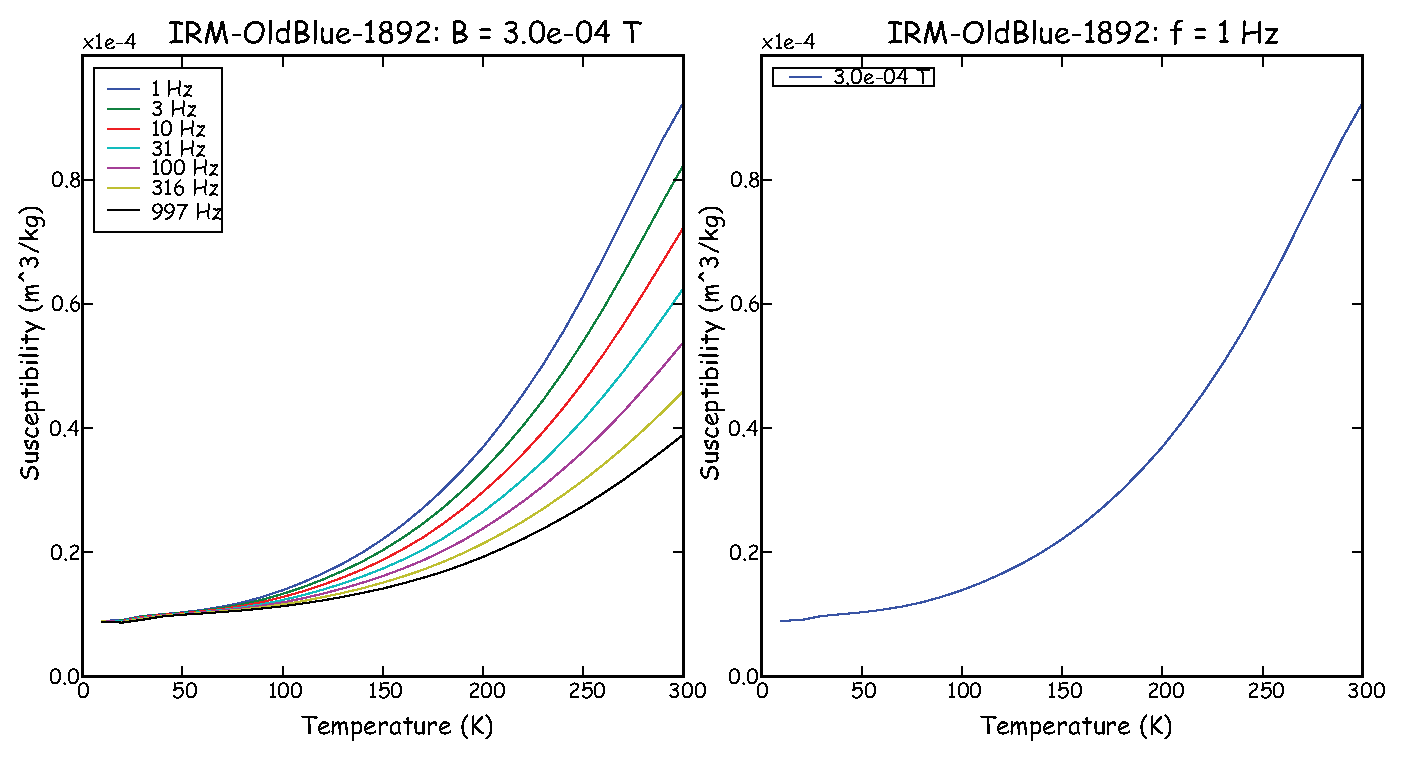
\includegraphics[width=20cm]{EPSfiles/chi-magic.eps}

You can see the dependence on temperature, frequency and applied field.  These data support the suggestion that there is a strong superparamagnetic component in these specimens.   

%\customlink{combine_magic}
\section {\bf combine\_magic.py} \href{#MagIC}{[MagIC]}
\label{ex:combine_magic}

MagIC tables have many columns only some of which are used in a particular instance.  So combining files of the same type must be done carefully to ensure that the right data come under the right headings.  The program {\bf combine\_magic.py} can be used to combine any number of MagIC files from a given type.    For an example of how to use this program, see Example~\ref{ex:agm_magic}. 

%\customlink{common_mean.py}
\section {\bf common\_mean.py} 
\href{http://magician.ucsd.edu/Essentials/WebBook2.html#Beyond_Fisher_statistics}{[Chapter 12]}

Most paleomagnetists use some form of Fisher Statistics to decide if two directions are statistically distinct or not (see \href{http://magician.ucsd.edu/Essentials/WebBook2.html#Fisher_statistics}{Chapter 11} for a discussion of those techniques.  But often directional data are not fisher distributed and the parametric approach will give misleading answers.  In these cases, one can use a boostrap approach, described in detail in \href{http://magician.ucsd.edu/Essentials/WebBook2.html#Beyond_Fisher_statistics}{[Chapter 12]}.  Here we
use the program {\bf common\_mean.py} for a bootstrap test for common mean to check whether two declination, inclination data sets have a common mean at the 95\% level of confidence.    The data sets are: {\it common\_mean\_ex\_file1.dat } and {\it common\_mean\_ex\_file2.dat}.  But first, let's look at the data in equal area projection  using the program \href{#eqarea.py}{eqarea.py}.

The session: 
\begin{verbatim}
% eqarea.py -f common_mean_ex_file1.dat -p
1  saved in  common_mean_ex_file1.dat.svg

%  eqarea.py -f common_mean_ex_file2.dat -p
1  saved in  common_mean_ex_file2.dat.svg
\end{verbatim} 

\noindent generates two .svg formatted files that look like these:

{%\epsfxsize 5cm
\hskip 1in %\epsffile{EPSfiles/common-mean-eq.eps}
  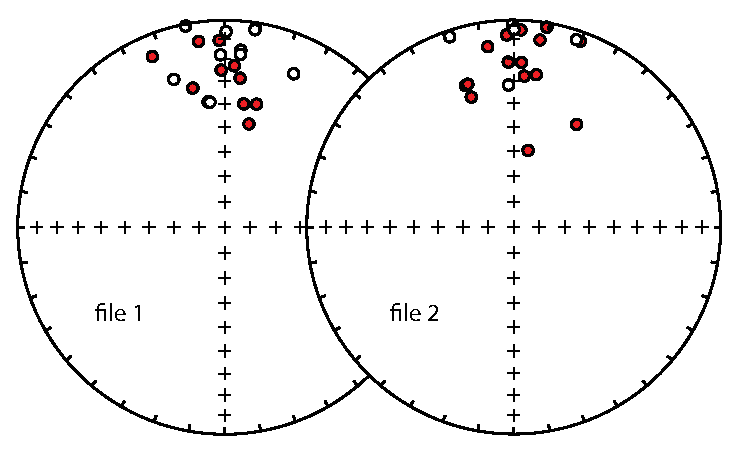
\includegraphics[width=15 cm]{EPSfiles/common-mean-eq.eps}}
  
Now let's look at the common mean problem using {\bf common\_mean.py}. 

\begin{verbatim}
% common_mean.py -f common_mean_ex_file1.dat -f2 common_mean_ex_file2.dat
Doing first set of directions, please be patient..
Doing second set of directions, please be patient..
S[a]ve plots, <Return> to quit
\end{verbatim}

\noindent The three plots are:

%\epsfxsize 14.5cm
{ %\epsffile{EPSfiles/common-mean.eps}
  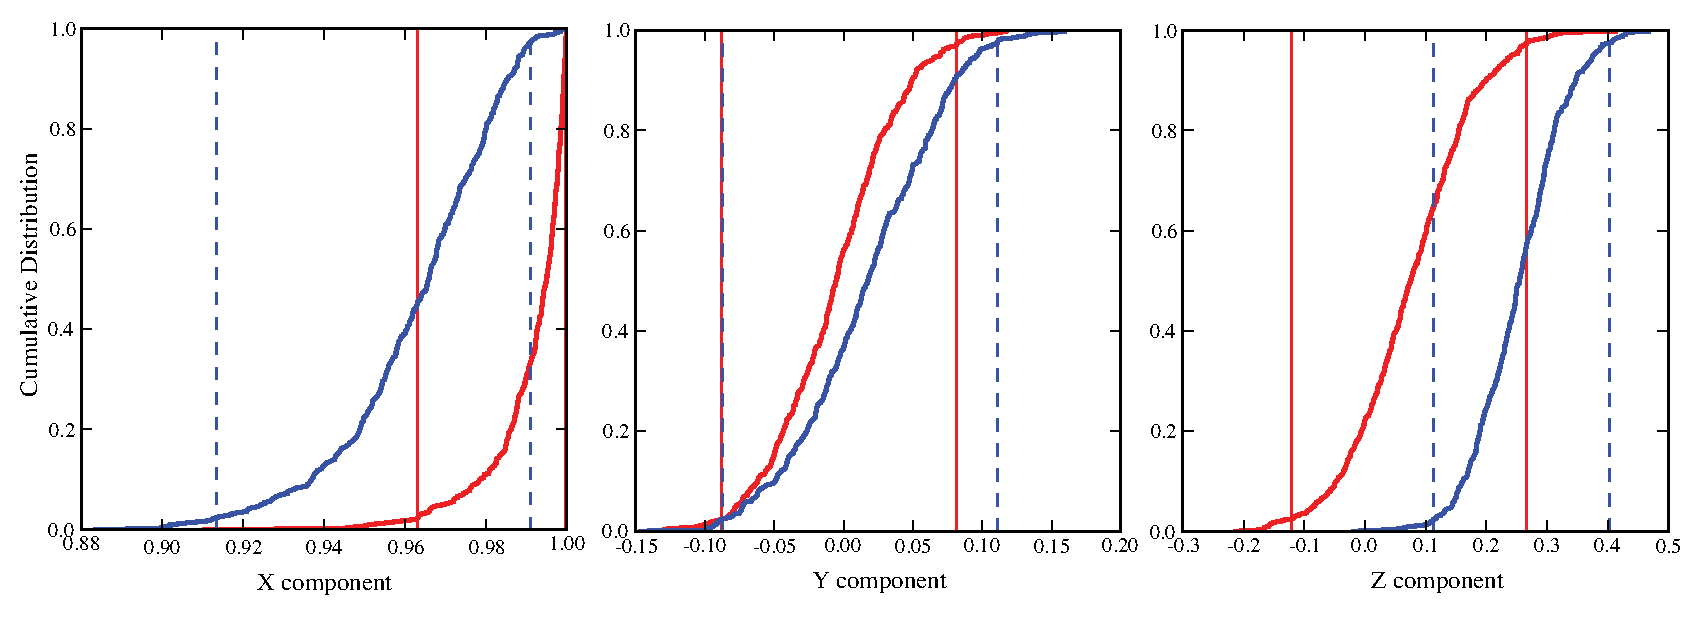
\includegraphics[width=20 cm]{EPSfiles/common-mean.eps}}

These suggest that  the two data sets share a common mean.  

Now compare the data in  {\it common\_mean\_ex\_file1.dat }  with the expected direction at the 5$^{\circ}$N latitude that these data were collected (Dec=0, Inc=9.9).   

To do this,  follow this transcript:

\begin{verbatim}
% common_mean.py -f common_mean_ex_file1.dat -dir 0 9.9
Doing first set of directions, please be patient..
S[a]ve plots, <Return> to quit
\end{verbatim}

%\epsfxsize 14.5cm
{% \epsffile{EPSfiles/common-mean-EX.eps}
  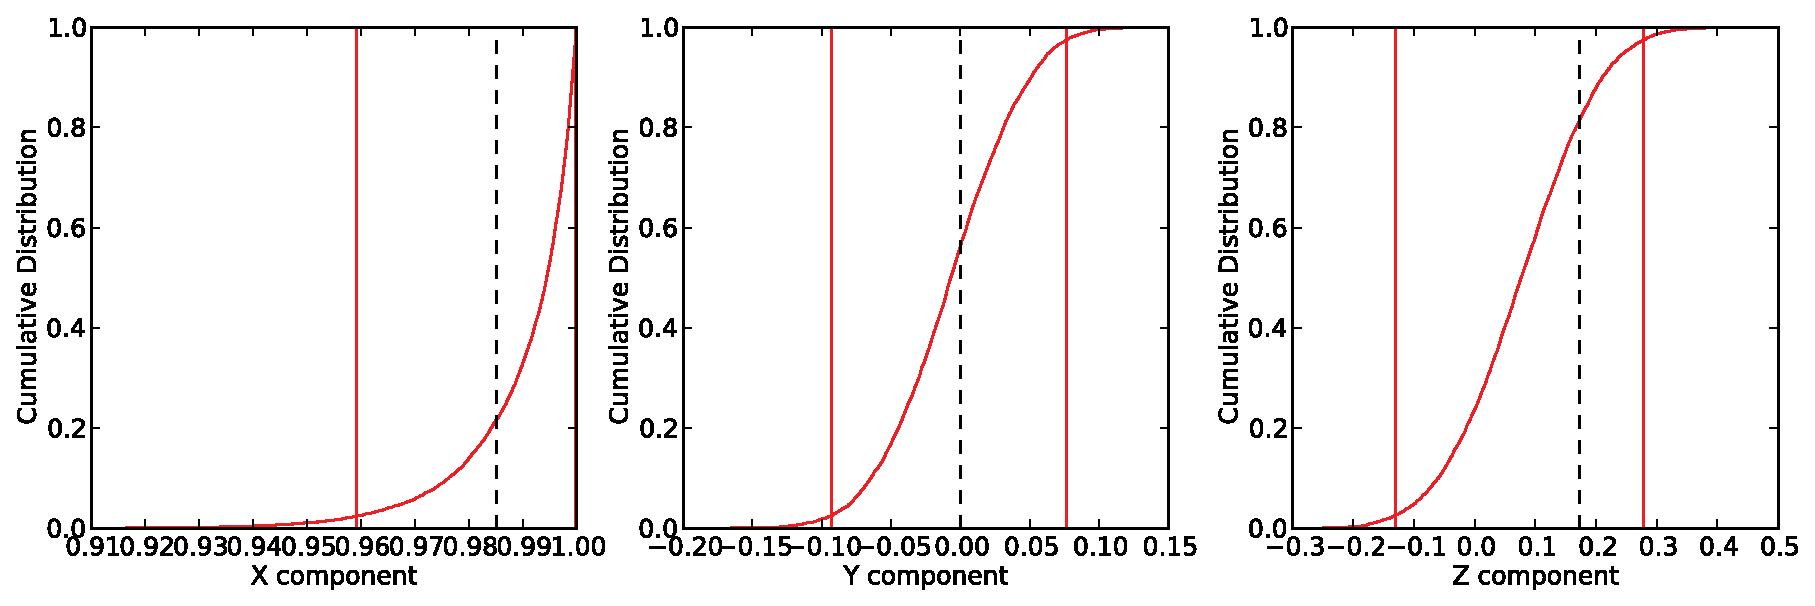
\includegraphics[width=20cm]{EPSfiles/common-mean-EX.eps}}

Apparently the data (cumulative distribution functions) are entirely consistent with the expected direction (dashed lines are the cartesian coordinates of that).   

%\customlink{cont_rot.py}
\section{cont\_rot.py} 
\href{http://Webbookcopy.html#Tectonic_applications_of_paleomagnetism}{[Chapter 16 }and \href{http://Webbookcopy.html#polerot}{Appendix A.3.5.]}

Use the program {\bf cont\_rot.py} to make an orthographic projection with latitude = -20$^{\circ}$ and longitude = 0$^{\circ}$ at the center of the African and South American  continents reconstructed to 180 Ma using the Torsvik et al. (2008) poles of finite rotation.  \nocite{torsvik08} Do this by first holding Africa fixed.  Move the output plot to {\it fixed\_africa.svg}.  Then make the plot for Africa adjusted  to the paleomagnetic reference frame.  Make the continental outlines in black lines and set the resolution to 'low'.  

\begin{verbatim}
% cont_rot.py -con af:sam -prj ortho -eye -20 0 -sym 'k-' 1 -age 180 -res l
 S[a]ve to save plot, Return to quit:  a
1  saved in  Cont_rot.pdf
% mv Cont_rot.pdf fixed_africa.pdf
% cont_rot.py -con af:sam -prj ortho -eye -20 0 -sym 'k-' 1 -age 180 \
     -res l -sac
 S[a]ve to save plot, Return to quit:  a
1  saved in  Cont_rot.pdf
\end{verbatim}

These commands generated the following plots (first on left, second on right):

{%\epsfxsize 12cm 
\hskip 1cm %\epsffile{EPSfiles/controt.eps}
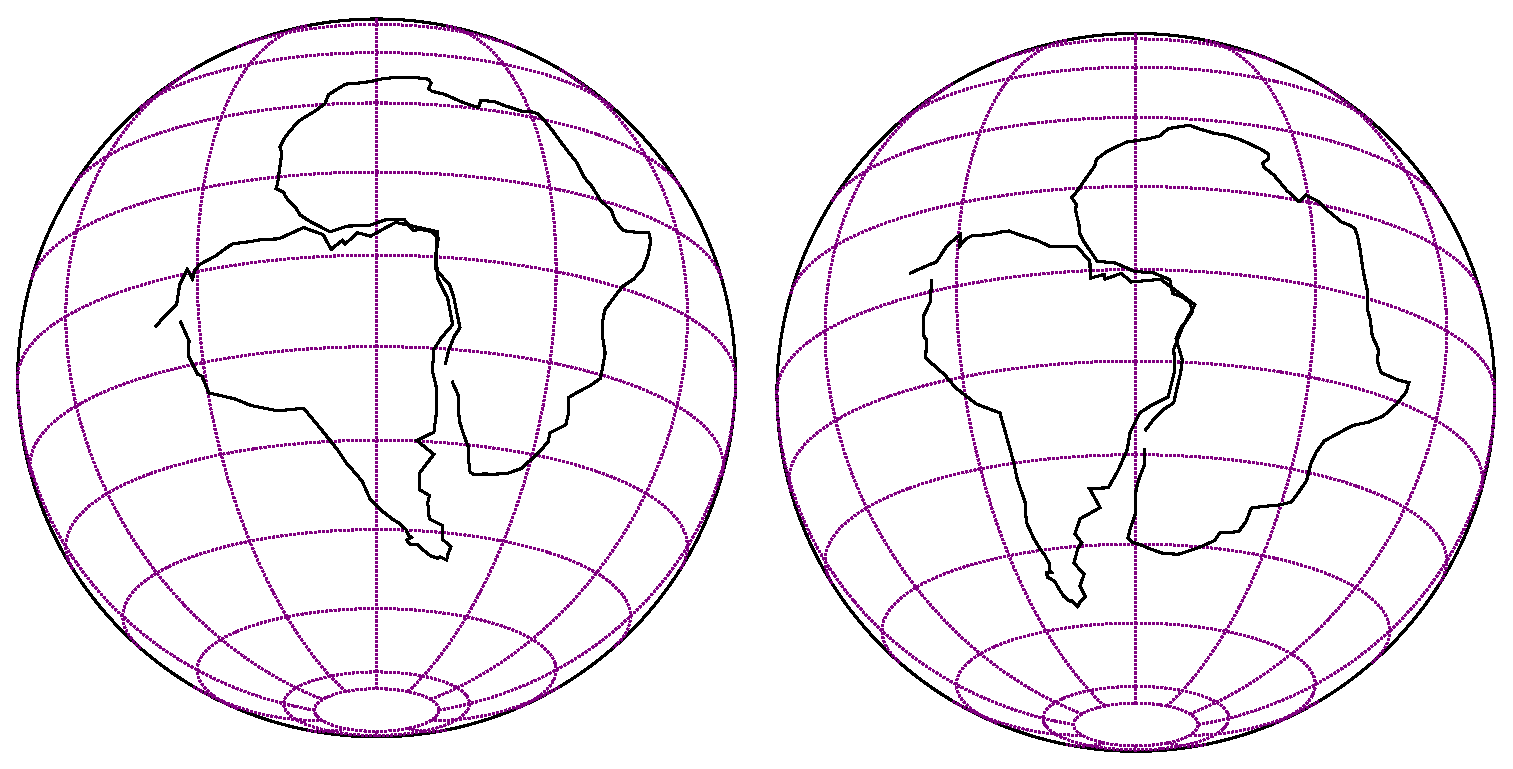
\includegraphics[width=15 cm]{EPSfiles/controt.eps}}

%\customlink{convert2unix.py}
\section{convert2unix.py}

This is a handy little script that turns Windows or Mac file formatted files (not Word or other proprietary formats) into Unix file format.  It does the change in place, overwriting the original file.

%\customlink{convert_samples.py}
\section{convert_samples.py}
\href{#MagIC}{[MagIC]}

If one of the MagIC related programs in PmagPy created a very lean looking {\it er\_samples.txt} file (for example using \href{#azdip_magic.py}{azdip\_magic.py}) and you need to add more information (say, latitude, longitude, lithology, etc.), you can convert the {\it er\_samples.txt} file into an \href{#orientation_magic.py}{orient.txt} file format, edit it in, for example Excel, and then re-import it back into the {\it er\_samples.txt} file format.  Try this on the {\it er\_samples} formatted file in the {\it convert\_samples} directory, {\it convert\_samples\_example.dat}.

\begin{verbatim}
% convert_samples.py -f convert_samples_example.dat 
Data saved in:  orient_Northern_Iceland.txt
\end{verbatim}




%\customlink{core_depthplot.py}
\section{core\_depthplot.py} [\href{http://magician.ucsd.edu/Essentials/WebBook2.html#The_GPTS_and_magnetostratigraphy}{Chapter 15}] 
\label{ex:core_depthplot}

Use the program {\bf core\_depthplot.py} to plot various measurement data versus sample depth.   The data must be in the MagIC data formats.  The program will plot whole core data, discrete sample at a bulk demagnetization step, data from vector demagnetization experiments, and so on.  There are many options, so check the help menu before you begin.     

We can try this out on some data from DSDP Hole 522, measured by Tauxe and Hartl (1997).  \nocite{tauxe97}  These can be downloaded and unpacked (see \href{#download_magic.py}{download-magic.py} for details,  or you can try it out on the data files in the directory {\bf core\_depthplot}.   You must specify a lab-protocol (LP) for plotting.  In this example, we will plot the alternating field (AF) data after the 15 mT step.  The magnetizations will be plotted on a log scale and, as this is a record of the Oligocene, we will plot the Oligocene time scale, using the calibration of Gradstein et al. (2004),  \nocite{gradstein04} commonly referred to as ``GTS04'' for the the Oligocene.  We are only interested in the data between 50 and 150 meters (the -d option sets this) and we will suppress the declinations (-D).  

\begin{verbatim}
core_depthplot.py -LP AF 15 -log -d 50 150 -ts gts04 23 34 -D
\end{verbatim}

\noindent  will produce the plot:

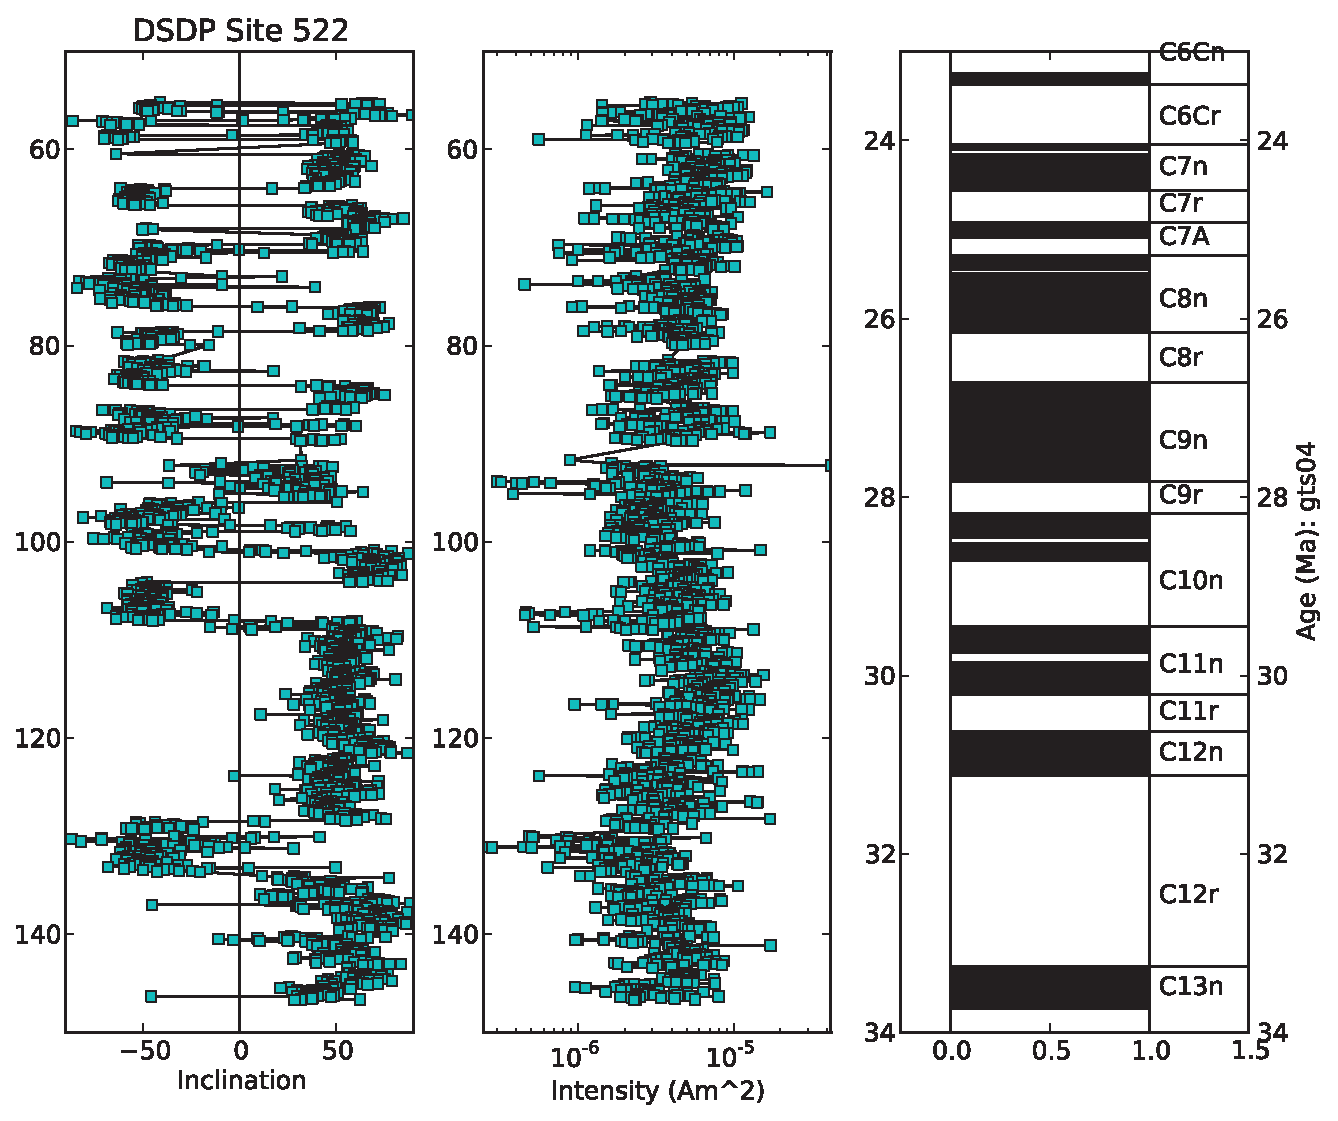
\includegraphics[width=15 cm]{EPSfiles/core-depthplot.eps}


%\customlink{curie.py}
\section{curie.py} 
\href{http://magician.ucsd.edu/Essentials/WebBook2.html#magnetic_mineralogy}{[Chapter 6]}
\label{ex:curie}
% NOTE TO SELF:  THIS NEEDS TO BE UPDATED USING THE BETTER METHOD OF EGLI (OR WAS IT HESLOP?) FOR CURIE T ESTIMATION

Use the program {\bf curie.py} to interpret curie temperature data in the example file {\it curie\_example.dat}.  Use a smoothing window of 10$^{\circ}$.



\begin{verbatim}
%curie.py -f curie_example.txt -w 10
second deriative maximum is at T=552
\end{verbatim}

\noindent which generates these plots:

%\epsfxsize 14.5cm
{%\epsffile{EPSfiles/curie-ex.eps}
  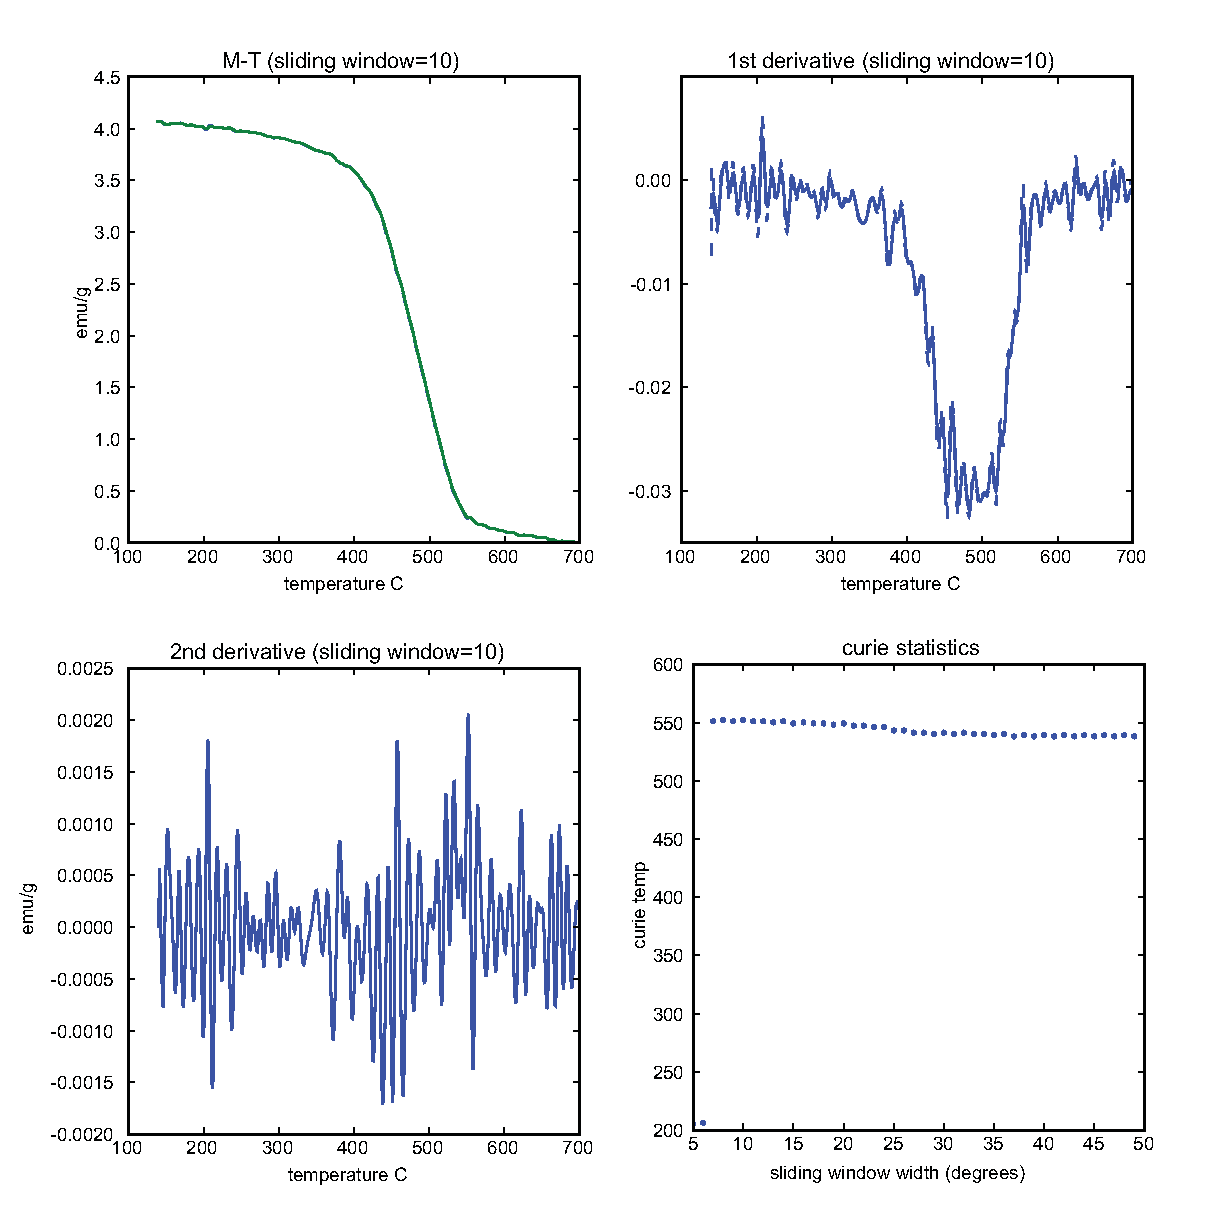
\includegraphics[width=14.5 cm]{EPSfiles/curie-ex.eps}}


%\customlink{customize_criteria.py}
\section{customize\_criteria.py} 
\href{#MagIC}{[MagIC]}
\label{ex:customize_criteria}

The MagIC database allows documentation of which criteria were used in selecting data on a specimen, sample or site level and to easily apply those criteria (and re-apply them as they change) in preparing the different tables.  These choices are stored in the {\it pmag\_criteria} table in each MagIC project directory (see \href{#MagIC.py}{MagIC.py} documentation.

 Certain {\bf PmagPy} programs use the datafile {\it pmag\_criteria.txt} to select data (for example {\bf thellier\_magic.py} and {\bf specimens\_results\_magic.py}).  To customize these criteria for your own data sets, you can use the program {\bf customize\_criteria.py}.  This program is also called by the {\bf MagIC.py} GUI under the Utilities menu.    Try it out on {\it pmag\_criteria.txt}.   This is a ``full vector'' set of criteria - meaning that it has both directions and intensity flags set.  Change the {\it specimen\_alpha95} cutoff to 180. from whatever it is now set to.   Save the output to a new file named {\it new\_criteria.txt}.

\begin{verbatim}
% customize_criteria.py -f pmag_criteria.txt -F new_criteria.txt
Acceptance criteria read in from  pmag_criteria.txt
 [0] Use no acceptance criteria?
 [1] full vector
 [2] direction only
 [3] intensity only 
 1
specimen_mad 5.49
Enter new criterion (return to keep default) 
specimen_alpha95 5.49
Enter new criterion (return to keep default) 180.
.
.
site_int_sigma_perc 15
Enter new criterion (return to keep default) 
Customize criteria again ? 1/[0]
Criteria saved in pmag_criteria.txt

 Pmag Criteria stored in  new_criteria.txt 

\end{verbatim}

Note that the default place for the PmagPy programs to look for criteria is in {\it pmag\_criteria.txt}, so you should probably rename the new one that for it to take effect as your new default.

%

%\customlink{dayplot_magic.py}
\section{dayplot\_magic.py}
\href{http://magician.ucsd.edu/Essentials/WebBook2.html#Magnetic_hysteresis}{[Chapter 5]} 

 Use the program {\bf dayplot\_magic.py}  to make Day, Squareness-Coercivity and Squareness-Coercivity of Remanence plots from the rmag\_hyseresis formatted data in {\it dayplot\_magic\_example.dat.}     
 
 The session:
 
  \begin{verbatim}
  % dayplot_magic.py -f dayplot_magic_example.dat

 S[a]ve to save plots, return to quit:  
\end{verbatim}
 
 
  
\noindent gives the plots:  

%\epsfxsize 14.5cm
{%\epsffile{EPSfiles/dayplot.eps}
  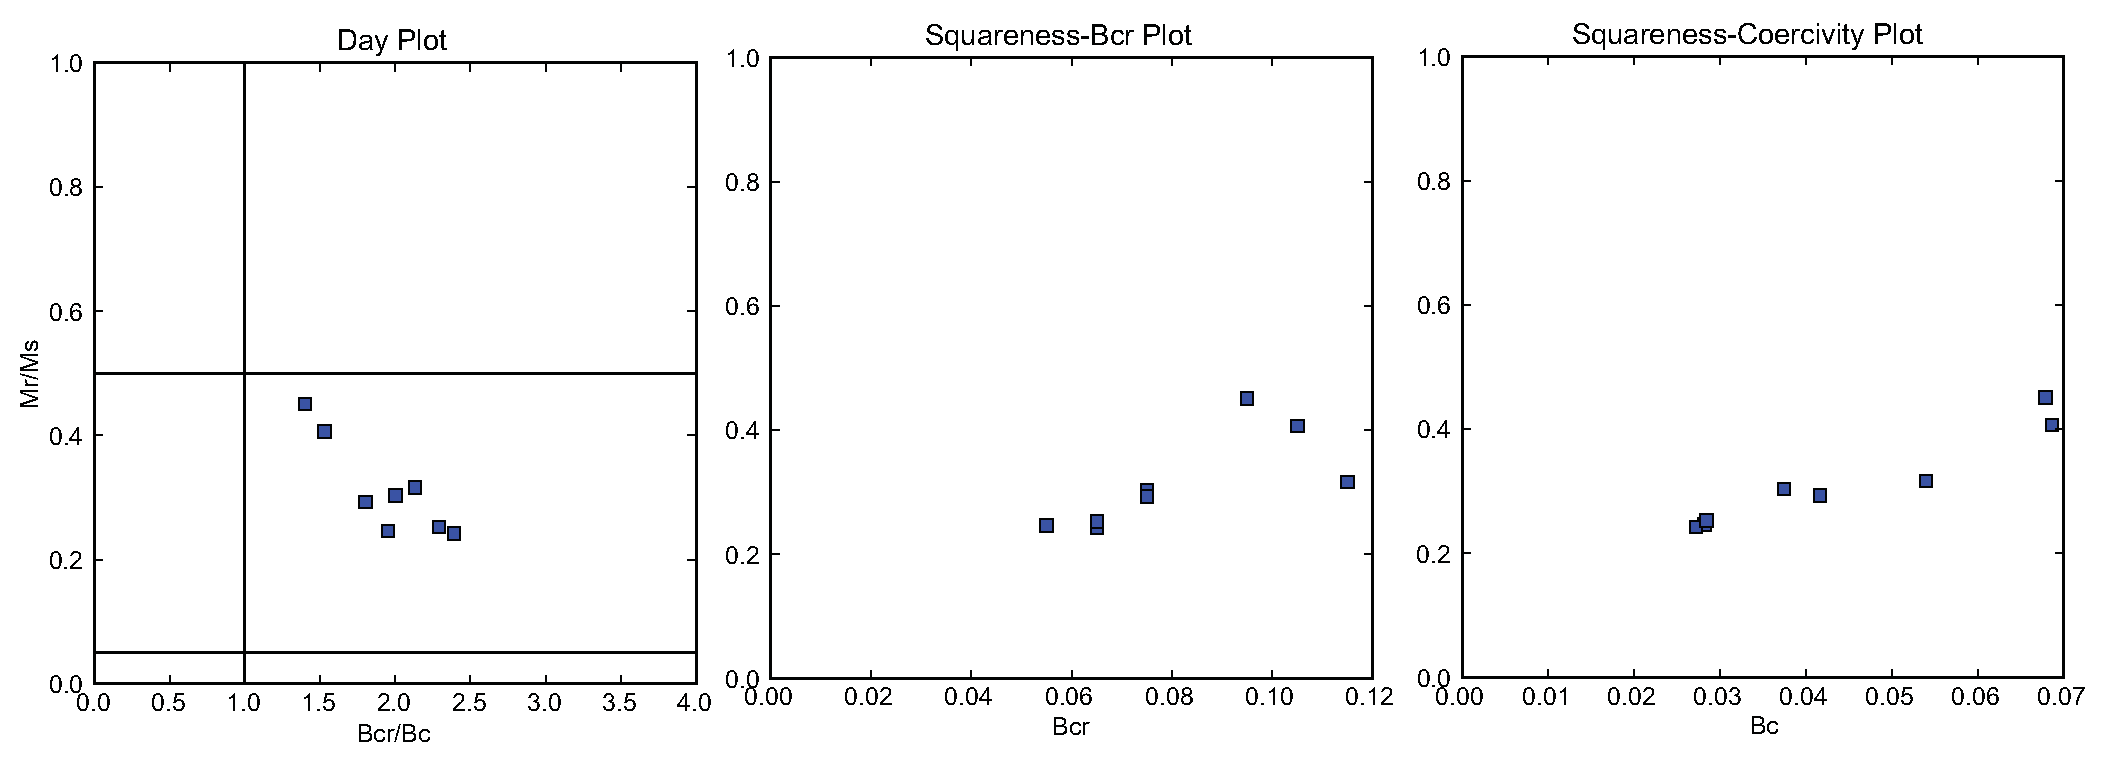
\includegraphics[width=20cm]{EPSfiles/dayplot.eps}}


%\customlink{di_eq.py}
\section{di\_eq.py}
\href{http://magician.ucsd.edu/Essentials/WebBook2.html#equal_area}{[Appendix B]}
\label{ex:di_eq}

Paleomagnetic data are frequently plotted in equal area projection.  PmagPy has several plotting programs which do this (e.g., \href{#eqarea.py}{eqarea.py}, but occasionally it is handy to be able to convert the directions to X,Y coordinates directly, without plotting them at all.  The program {\bf di\_eq.py} does this.  Here is an example transcript of a session using the datafile {\it di\_eq\_example.dat}:

\begin{verbatim}
% di_eq.py -f di_eq_example.dat
-0.239410 -0.893491
0.436413 0.712161
0.063844 0.760300
0.321447 0.686216
0.322720 0.670562
0.407412 0.540654
.
.
.
\end{verbatim}

%\customlink{di_geo.py}
\section {\bf di\_geo.py} 
\href{http://magician.ucsd.edu/Essentials/WebBook2.html#Getting_a_paleomagnetic_direction}{[Chapter 9]} and
\href{http://magician.ucsd.edu/Essentials/WebBook2.html#Changing_coordinate_systems}{Changing coordinate systems}
\label{ex:di_geo}

Use the programs {\bf di\_geo.py}  to convert
$D=8.1, I=45.2$ from specimen coordinates  to geographic  adjusted coordinates. The
orientation of laboratory arrow on the specimen was: azimuth = 347;
plunge = 27.  
{\bf di\_geo.py} works in the usual three ways (interactive data entry, command line file specification or from standard input.  So for a quickie answer for a single specimen, you can use the interactive mode:

\begin{verbatim}
% di_geo.py -i
Declination: <cntrl-D> to quit  81
Inclination: 45.2
Azimuth: 347
Plunge: 27
   94.8    43.0
\end{verbatim}
\noindent which spits out our answer of Declination = 5.3 and inclination = 71.6.  

For more data, it is handy to use the file entry options. There are a bunch of declination, inclination, azimuth and plunge data in the file {\it di\_geo\_example.dat} in the {\it di\_geo} directory.  First look at the data in specimen coordinates in equal area projection, using the program \href{#eqarea.py}{eqarea.py}.  Note that this program only pays attention to the first two columns so it will ignore the orientation information. 

\begin{verbatim}
% eqarea.py -f di_geo_example.dat
\end{verbatim}
which should look like this:  

  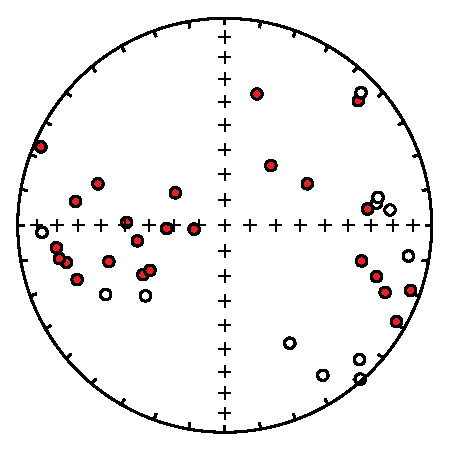
\includegraphics[width=10 cm]{EPSfiles/di_geo_spc_eq.eps}



The data are highly scattered and we hope that the geographic coordinate system looks better!  To find out try:
\begin{verbatim}
di_geo.py -f di_geo_example.dat >di_geo.out;  eqarea.py -f di_geo.out

\end{verbatim}

\noindent which looks like this:

  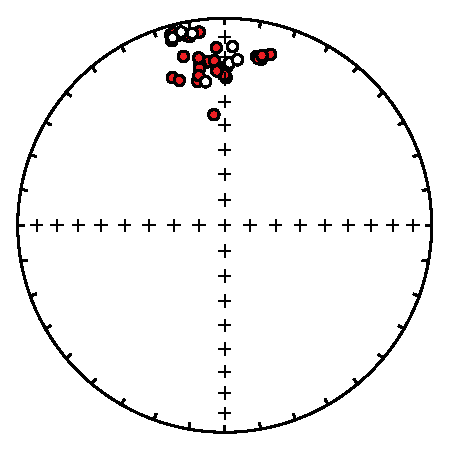
\includegraphics[width=10cm]{EPSfiles/di_geo_geo_eq.eps}
  
  \noindent These data are clearly much better grouped.  



%\customlink{di_rot.py}
\section{di\_rot.py}
\href{http://Webbook2.html/#Fisher_statitstics}{ [Chapter  11]}


Generate a Fisher distributed set of data from a population with a mean direction of $D=0, I=42$ using the program {\bf fishrot.py}.  Calculate the mean direction of the data set using {\bf gofish.py}.  Now use the program \href{#di_rot.py}{di\_rot.py} to rotate the set of directions to the mean direction.  Look at the data before and after rotation using \href{#eqarea.py}{eqarea.py}.  

\begin{verbatim}
% fishrot.py -I 42 >fishrot.out
% gofish.py <fishrot.out
    1.7    42.4    100    95.3720     21.4     3.1
% di_rot.py -f fishrot.out -F dirot.out -D 1.7 -I 42.4
% eqarea.py -f fishrot.out
 % eqarea.py -f dirot.out
\end{verbatim}

\noindent  which generates plots like these:

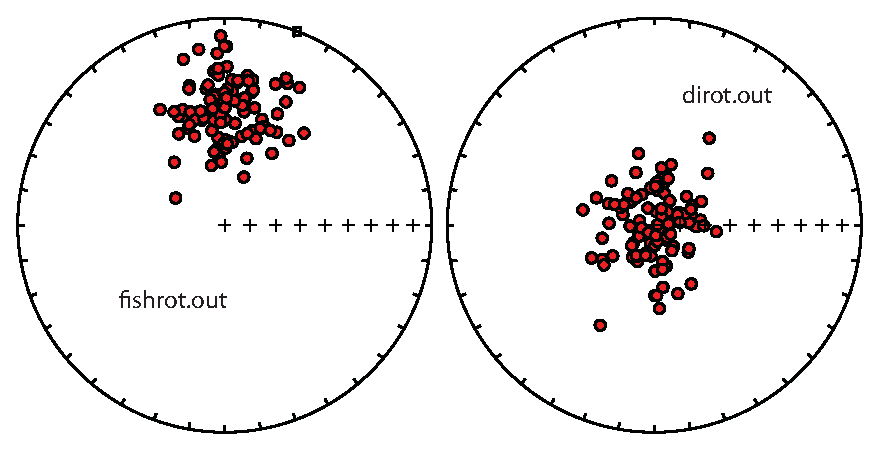
\includegraphics[width=15 cm]{EPSfiles/dirot.eps}}

Note that every instance of {\bf fisher.py} will draw a different sample from a Fisher distribution and your exact plot and average values will be different in detail every time you try this (and that's part of the fun of statistical simulation.)


%\customlink{di_tilt.py}
\section {\bf di\_tilt.py} 
\href{http://magician.ucsd.edu/Essentials/WebBook2.html#Getting_a_paleomagnetic_direction}{[Chapter 9]} and
\href{http://magician.ucsd.edu/Essentials/WebBook2.html#changing_coordinate_systems}{Changing coordinate systems}
\label{ex:di_tilt}


Use the program {\bf di\_tilt.py} to rotate a direction of Declination = 5.3 and Inclination = 71.6 to ``stratigraphic'' coordinates.  The  strike was 135 and the dip was 21.
The convention  in this program is to use  the dip direction, which  is to the ``right'' of 
this strike.    


Here is  a session with {\bf di\_tilt.py} using the interactive option:

\begin{verbatim}
% di_tilt.py -i
Declination: <cntl-D> to quit 5.3
Inclination: 71.6
Dip direction: 225
Dip: 21
  285.7    76.6
Declination: <cntl-D> to quit ^D
 Good-bye
\end{verbatim}  

Try the same on the data file saved as {\it di\_tilt\_example.dat} using the command line -f switch:



%\customlink{di_vgp.py}
\section{di\_vgp.py}
\href{http://Webbook2.html/#Virtual_geomagnetic_poles}{[Chapter  2]}

Use the program {\bf di\_vgp} to convert the
following:

\begin{center}
\begin{tabular}{rrrr}
\hline
$D$ & $I$ & $\lambda_s$ (N) & $\phi_s$ (E)\cr
\hline
11 & 63  & 55 & 13\cr
154  & -58    & 45.5 & -73  \cr
\hline
\end{tabular}
\end{center}

Here is a transcript of a typical session using the command line option for file name entry: 

\begin{verbatim}
% di_vgp.py -f di_vgp_example.dat
  154.7    77.3
    6.6   -69.6
\end{verbatim}

%\customlink{dipole_pinc.py}
\section {\bf dipole\_pinc.py}
\href{http://Webbook2.html/#Virtual_geomagnetic_poles}{[Chapter  2]}

Calculate the expected inclination at a paleolatitude of 24$^{\circ}$S.

\begin{verbatim}
% dipole_pinc.py -i
Paleolat for converting to inclination: <cntl-D> to quit -24
  -41.7
Paleolat for converting to inclination: <cntl-D> to quit ^D
 Good-bye 

\end{verbatim}

%\customlink{dipole_plat.py}
\section {\bf dipole\_plat.py}
\href{http://Webbook2.html/#Virtual_geomagnetic_poles}{[Chapter  2]}

Calculate the paleolatitude for an average inclination of 23$^{\circ}$.  

\begin{verbatim}
% dipole_plat.py -i
Inclination for converting to paleolatitude: <cntl-D> to quit 23
   12.0
Inclination for converting to paleolatitude: <cntl-D> to quit ^D
 Good-bye 
\end{verbatim}

%\customlink{dir_cart.py}
\section {\bf dir\_cart.py} [\href{http://magician.ucsd.edu/Essentials/WebBook2.html#The_geomagnetic_field}{Chapter 2}]
\label{ex:dir_cart}

Use the program {\bf dir\_cart.py} to convert the
following data from declination $D$, inclination $I$ and intensity
$M$ to $x_1,x_2,x_3$.


\begin{tabular}{ccc}
\hline
$D$ & $I$ &  $M$ ($\mu \hbox{Am}^2$)\cr
\hline
20 & 46 & 1.3\cr
175 & -24 & 4.2\cr
\hline
\end{tabular}

You can enter $D,I,M$ data into data file, then running the program by typing what is after the prompts (\%) [ the other stuff is computer responses] :

\begin{verbatim}
% cat > dir_cart_example.dat
 20 46 1.3
175 -24 4.2 
^D
% dir_cart.py <dir_cart_example.dat 
8.4859e-01 3.0886e-01 9.3514e-01
-3.8223e+00 3.3441e-01 -1.7083e+00
\end{verbatim} 

 Or you could use {\bf dir\_cart.py} interactively as in:
 
 \begin{verbatim}
 % dir_cart.py -i

Declination: [cntrl-D  to quit] 
 Good-bye 

% dir_cart.py -i
Declination: [cntrl-D  to quit] 20
Inclination: 46
Intensity [return for unity]: 1.3
8.4859e-01 3.0886e-01 9.3514e-01
Declination: [cntrl-D  to quit] 175
Inclination: -24
Intensity [return for unity]: 4.2
-3.8223e+00 3.3441e-01 -1.7083e+00
Declination: [cntrl-D  to quit] ^D
 Good-bye 
\end{verbatim}

% 
% 
%\customlink{dmag_magic.py}
 \section {\bf dmag\_magic.py}
  [\href{http://Webbookcopy.html#Getting_Direction}{Chapter 9} and \href{#MagIC}{[MagIC]}
 
Use {\bf dmag\_magic.py} to plot out the decay of all alternating field demagnetization experiments in the magic\_measurements 
formatted file in {\it dmag\_magic\_example.dat}.    Repeat for all thermal measurements, but exclude all the data acquired during the thermal but not  paleointensity experiments.   Try this at the location level and then at the site level. 

Here is a transcript of a session:

\begin{verbatim}
%  dmag_magic.py -f dmag_magic_example.dat -LT AF
5921  records read from  dmag_magic_example.dat
McMurdo plotting by:  er_location_name
 S[a]ve to save plot, [q]uit,  Return to continue:  a
1  saved in  McMurdo_LT-AF-Z.svg
% dmag_magic.py -f dmag_magic_example.dat -LT T -XLP PI
5921  records read from  dmag_magic_example.dat
McMurdo plotting by:  er_location_name
 S[a]ve to save plot, [q]uit,  Return to continue:  a
1  saved in  McMurdo_LT-T-Z.svg
% dmag_magic.py -f dmag_magic_example.dat -LT AF -obj sit
5921  records read from  dmag_magic_example.dat
mc20 plotting by:  er_site_name
 S[a]ve to save plot, [q]uit,  Return to continue:   
mc200 plotting by:  er_site_name
 S[a]ve to save plot, [q]uit,  Return to continue:  a
1  saved in  mc200_LT-AF-Z.svg

\end{verbatim}

\noindent which produced these plots:

%\epsfxsize 12cm
{\hskip 1cm %\epsffile{EPSfiles/dmag.eps}
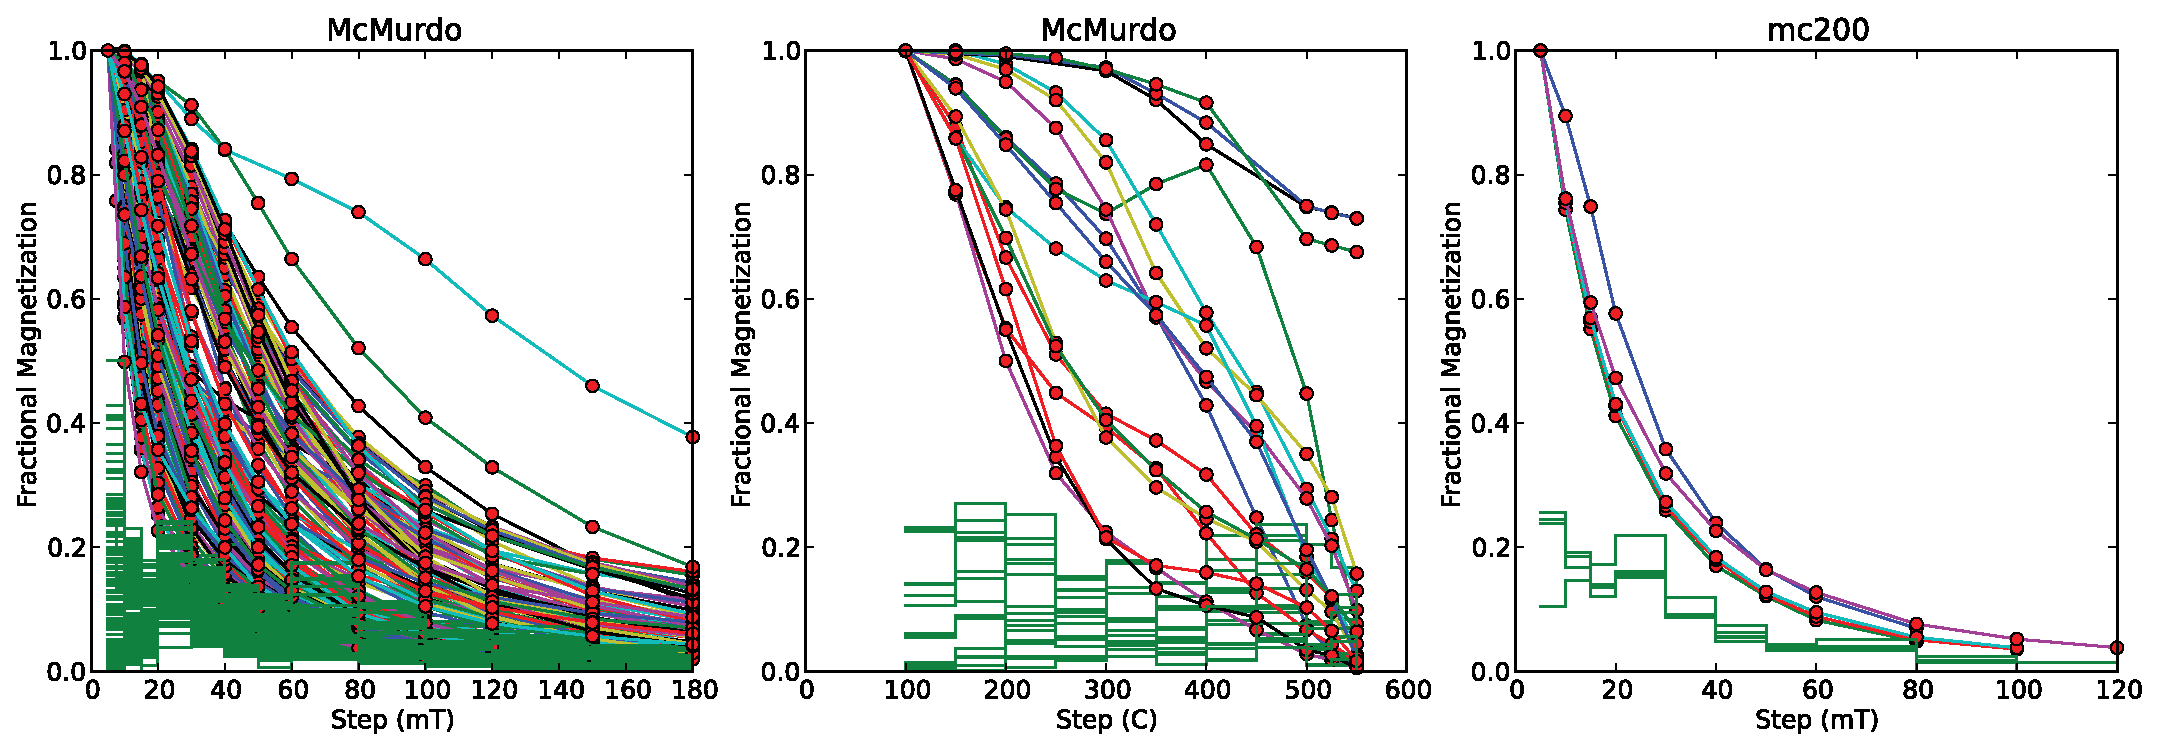
\includegraphics[width=20 cm]{EPSfiles/dmag.eps}}

%\customlink{download_magic.py}
 \section  {\bf download\_magic.py} [\href{http://earthref.org/MagIC}{MagIC}]
 \label{ex:download_magic}
 
 This program unpacks .txt files downloaded from the MagIC database into individual directories for each location into which the individual files for each table (e.g., {\it er\_locations.txt, magic\_measurements.txt, pmag\_results.txt} and so on) get placed.   As an example, go to the MagIC data base at \url{http://earthref.org/MAGIC/search}.  Enter ``Tauxe and 2004'' into the Reference Text Search field. 
 Show you several references.   Look for the one for Tauxe, L., Luskin, C., Selkin, P., Gans, P. and Calvert, A. (2004).  Download the  text file under the "Contribution SmartBook'' column and save it to your desktop.   Make a   folder into which  you should put the downloaded txt file called MagIC\_download and move the file into it.  Now use the program {\bf download\_magic.py} to unpack the .txt file ({\it zmab0083201tmp03.txt}).   
 
 \begin{verbatim}
% mkdir MagIC_download
% cd MagIC_download
% download_magic.py -f zmab0083201tmp03.txt
% download_magic.py -f zmab0083201tmp03.txt 
working on:  'er_locations'
er_locations  data put in  ./er_locations.txt
working on:  'er_sites'
er_sites  data put in  ./er_sites.txt
working on:  'er_samples'
er_samples  data put in  ./er_samples.txt
working on:  'er_specimens'
.
.
.
location_1:  Snake River
unpacking:  ./er_locations.txt
1  read in
1  stored in  ./Location_1/er_locations.txt
unpacking:  ./er_sites.txt
27  read in
27  stored in  ./Location_1/er_sites.txt
unpacking:  ./er_samples.txt
271  read in
271  stored in  ./Location_1/er_samples.txt
unpacking:  ./er_specimens.txt
.
.
.
\end{verbatim}

You can change directories each Location directory (in this case only one) and examine the data using the {\bf PmagPy} programs (e.g., \href{#zeq_magic.py}{zeq\_magic.py}).   


 % 
 %\customlink{eigs_s.py}
\section {\bf eigs\_s.py}
\href{http://Webbook2.html#Paleomagnetic_tensors}{ [Chapter 13]}

Print out the eigenparameters  in the file {\it eigs\_s\_example.dat} and then
convert them to tensor data in the .s format (x11,x22,x33,x12,x13,x23).   

This session uses the unix utility {\bf cat} to print the data.  [ You could use the Ms-Dos 
form {\bf type} in a Windows command line window.]    Then, it prints the tensor data to the screen.  

\begin{verbatim}
% cat eigs_s_example.dat 
0.33127  239.53   44.70 0.33351  126.62   21.47 0.33521  19.03   37.54
0.33177  281.12    6.18 0.33218  169.79   73.43 0.33603   12.82   15.32
...
% eigs_s.py -f eigs_s_example.dat
0.33416328 0.33280227 0.33303446 -0.00016631 0.00123163 0.00135521 
0.33555713 0.33197427 0.33246869 0.00085685 0.00025266 0.00098151 
0.33585301 0.33140355 0.33274350 0.00132308 0.00117787 0.00000455 
...
\end{verbatim}

%\section {\bf endnote\_magic.py} [MagIC]

%This handy program converts your EndNote reference data base bibtex formatted output to the MagIC er\_citations table format.    Try it on the file {\it EndNoteExport.txt}:

%\begin{verbatim}
%% endnote_magic.py
%Citations saved in  er_citations.txt
%\end{verbatim}

%You will  have to modify the er\_citation\_name to ``This study'' for the key reference  to the study you are trying to upload.  

%
%\customlink{eq_di.py}
\section {\bf eq\_di.py} [Appendix~\ref{app:eqarea}]

Data are frequently  published as equal area projections and not listed in data tables.  These data can be digitized as x,y data (assuming the outer rim is unity) and converted to approximate directions with the program {\bf eq\_di.py}.  To use this program, install a graph digitizer (GraphClick from \url{http://www.arizona-software.ch/graphclick/} works on Macs ).

Digitize the data from the equal area projection saved in the file {\it eqarea.png} in the {\it eq\_di} directory.
You should only work on one hemisphere at a time (upper or lower) and save each hemisphere in its own file.  Then you can convert the X,Y data to approximate dec and inc data - the quality of the data depends on your care in digitizing and the quality of the figure that you are digitizing.  

Try out {\bf eq\_di.py} on your datafile, or use {\it eq\_di\_example.dat} which are the digitized data from the lower hemisphere and check your work with {\bf eqarea.py}.  You should retrieve the lower hemisphere points from the {\bf eqarea.py} example.  

\begin{verbatim}
% eq_di.py -f eq_di_example.dat >tmp
% eqarea.py -f tmp
\end{verbatim}

NB: To indicate that your data are UPPER hemisphere (negative inclinations), use the -up switch.  

\section {\bf di\_eq.py} [Appendix~\ref{app:eqarea}]

This program takes declination, inclination data and converts them to X,Y pairs using the equal area projection.   Test this out with {\it di\_eq\_example.dat}.  These are the lower hemisphere data from {\it di\_example.dat}.  

\begin{verbatim}
% di_eq.py -f di_eq_example.dat >tmp
% cat tmp
0.436413031037 0.712161340983
0.0638442163337 0.760300494699
0.321447089986 0.68621605692
0.322719926466 0.670562477292
0.407412231411 0.540654291959
0.580156197966 0.340375619675
%.
%.
%.
%\end{verbatim}

You can verify the process by comparing the plot generated for these data using \href{#eqarea.py}{eqarea.py} with the original png file.  


%
%\customlink{eqarea.py}
\section {\bf eqarea.py}
\href{http://Webbook2.html#The_geomagnetic_field}{ [Chapter 2}and 
\href{http://Webbook2.html#Plots_useful_in_paleomagnetism}{[Appendix B.1]}

Use the program \href{#fishrot.py}{fishrot.py} to generate a Fisher distiributed set of data drawn from a distribution with mean declination of 42$^{\circ}$ and a mean inclination of 60$^{\circ}$.  LSave this to a file called {it fishrot.out}.   Use {\bf eqarea.py} to 
plot an equal area projection of the data.

\begin{verbatim}
%fishrot.py -D 42 -I 60 > fishrot.out
% eqarea.py -f fishrot.out
\end{verbatim}

\noindent
which produces the plot:

 %\epsffile{EPSfiles/eqarea.eps}
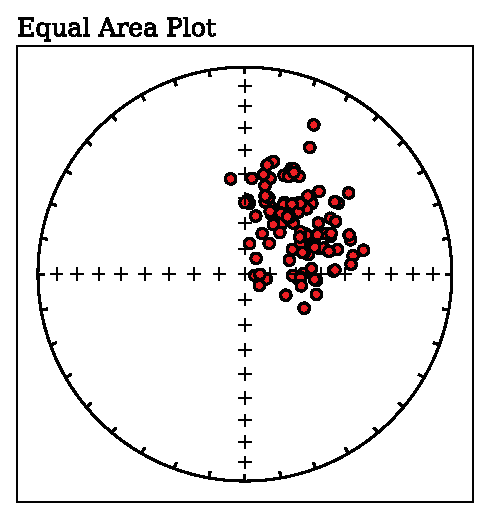
\includegraphics[width=10 cm]{EPSfiles/eqarea.eps}

%\customlink{eqarea_ell.py}
\section {\bf eqarea\_ell.py}
\href{http://Webbook2.html#Fisher_statistics}{ [Chapters 11]} and \href{http://Webbook2.html#Beyond_Fisher_statistics}{ [Chapter 12]}

Use the program \href{#tk03.py}{tk03.py} to generate a set of simulated data for a latitude of 42$^{\circ}$N including reversals.  
Then use the program {\bf eqarea\_ell.py} to 
plot an equal area projection of the directions in {\it di\_example.txt} and plot confidence ellipses.  Here is an example for
Bingham ellipses.  


\begin{verbatim}
% tk03.py -lat 42 -rev >tk03.out
% eqarea_ell.py -f tk03.out -ell B
     Zdec    21.0
     Edec   105.7
     Eta     4.5
     n        20
     Einc    10.0
     Zinc   -27.6
     Zeta     4.5
     dec   357.8
     inc    60.3
 S[a]ve to save plot, [q]uit, Return to continue:  a
1  saved in  tk03.out_eq.svg
\end{verbatim}

which produces a plot like this:

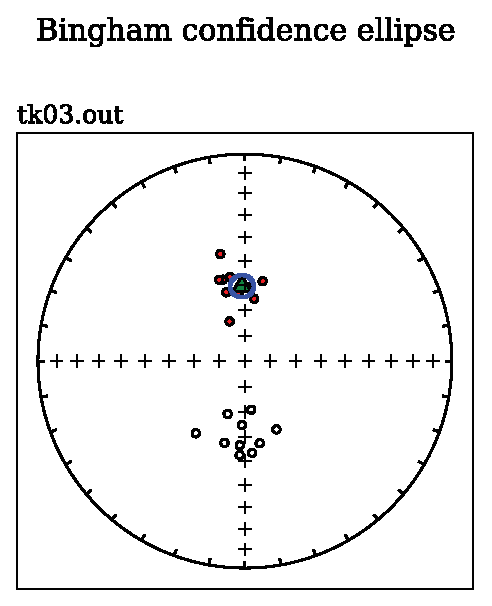
\includegraphics[width=10 cm]{EPSfiles/eqarea_ell.eps}

Other ellipses are Kent, Fisher and bootstrapped ellipses.  Check the documentation for details.

%\customlink{eqarea_magic.py}
\section {\bf eqarea\_magic.py} \href{#MagIC}{[MagIC]}

Follow the instructions for downloading and unpacking a data file from the MagIC database or use the file in the {\it download\_magic} directory already downloaded from the  \href{http://earthref.org/MagIC/search}{MagIC} website.    Plot the directional data for the study from the {\it pmag\_results.txt} file along with the bootstrapped 
 confidence ellipse.   

\begin{verbatim}
% eqarea_magic.py -obj loc -crd g -f pmag_results.txt -ell Be
24  records read from  ./pmag_results.txt
All
sr01 GM-ARAR-AP:LP-DC5:LP-DIR-AF:LP-DIR-T:LP-PI-ALT-PTRM:LP-PI-TRM-ZI   330.1    64.9
sr03 GM-ARAR-AP:LP-DC5:LP-DIR-AF:LP-DIR-T   151.8   -57.5
sr04 GM-ARAR-AP:LP-DC5:LP-DIR-AF:LP-DIR-T    16.5    54.6
.
.
.
sr31 GM-ARAR-AP:LP-DC5:LP-DIR-AF:LP-DIR-T    23.2    54.0
sr34 GM-ARAR-AP:LP-DC5:LP-DIR-AF:LP-DIR-T:LP-PI-ALT-PTRM:LP-PI-TRM-ZI   205.8   -49.4
sr36 GM-ARAR-AP:LP-DC5:LP-DIR-AF:LP-DIR-T   197.6   -65.5
sr39 GM-ARAR-AP:LP-DC5:LP-DIR-AF:LP-DIR-T:LP-PI-ALT-PTRM:LP-PI-TRM-ZI   188.1   -47.2
sr40 GM-ARAR-AP:LP-DC5:LP-DIR-AF:LP-DIR-T   192.9   -60.7
Normal Pole GM-ARAR-AP:LP-DC5:LP-DIR-AF:LP-DIR-T     6.1    59.6
Reverse pole GM-ARAR-AP:LP-DC5:LP-DIR-AF:LP-DIR-T   185.1   -58.8
Grand Mean pole GM-ARAR-AP:LP-DC5:LP-DIR-AF:LP-DIR-T     5.7    59.3
mode  1
     Zdec   111.1
     Edec   206.0
     Eta     7.8
     n        1
     Einc    28.9
     Zinc     8.7
     Zeta     3.3
     dec     6.0
     inc    59.6
mode  2
     Zdec   248.0
     Edec   150.1
     Eta     4.3
     n        1
     Einc    26.4
     Zinc    15.4
     Zeta     8.0
     dec   185.1
     inc   -58.8
 S[a]ve to save plot, [q]uit, Return to continue:  a
1  saved in  LO:_Snake River_SI:__SA:__SP:__CO:_gu_TY:_eqarea_.svg
\end{verbatim}

\noindent makes this plot:

%\epsfxsize 7cm
{\hskip 3.5cm %\epsffile{EPSfiles/eqarea-magic.eps}
 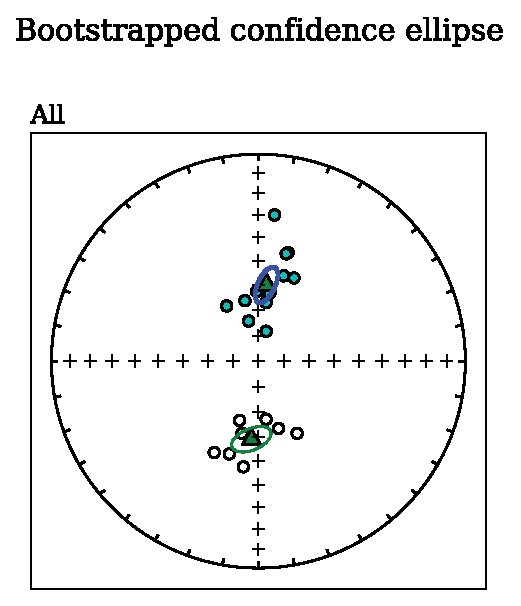
\includegraphics[width=10 cm]{EPSfiles/eqarea-magic.eps}}

The information printed to the window is the pmag\_result\_name in the data table, the method codes (here the geochronology method, the type of demagnetization code and the types of demagnetization experiments), and each site mean declination  inclination.    The information following ``mode 1'' are the bootstrapped ellipse parameters.

Some data are study averages and some are individual sites.
 
 Use \href{#magic_select.py}{magic\_select.py} to select only the individual site data.  Try the 
 
 \begin{verbatim}
 % magic_select.py -f pmag_results.txt -key data_type i 'T' -F site_results.txt
% eqarea_magic.py -f site_results.txt -ell Bv
21  records read from  ./site_results.txt
All
sr01 GM-ARAR-AP:LP-DC5:LP-DIR-AF:LP-DIR-T:LP-PI-ALT-PTRM:LP-PI-TRM-ZI   330.1    64.9
sr03 GM-ARAR-AP:LP-DC5:LP-DIR-AF:LP-DIR-T   151.8   -57.5
sr04 GM-ARAR-AP:LP-DC5:LP-DIR-AF:LP-DIR-T    16.5    54.6
sr09 GM-ARAR-AP:LP-DC5:LP-DIR-AF:LP-DIR-T    14.6    77.9
.
.
.
sr36 GM-ARAR-AP:LP-DC5:LP-DIR-AF:LP-DIR-T   197.6   -65.5
sr39 GM-ARAR-AP:LP-DC5:LP-DIR-AF:LP-DIR-T:LP-PI-ALT-PTRM:LP-PI-TRM-ZI   188.1   -47.2
sr40 GM-ARAR-AP:LP-DC5:LP-DIR-AF:LP-DIR-T   192.9   -60.7
 S[a]ve to save plot, [q]uit, Return to continue:  a
1  saved in  LO:_Snake River_SI:__SA:__SP:__CO:_g_TY:_eqarea_.svg
2  saved in  LO:_Snake River_SI:__SA:__SP:__CO:_g_TY:_bdirs_.svg
\end{verbatim}

which produces plots like:

 \includegraphics[width=15 cm]{EPSfiles/eqarea_magic_BV.eps}}

%\customlink{extract_methods.py}
\section{extract\_methods.py}
\href{#MagIC}{MagIC}

This script reads in any MagIC formatted table and extracts a list of unique method codes.




%\customlink{find_EI.py}
\section {\bf find\_EI.py}
 \href{http://Webbook2.html#The_ancient_geomagnetic_field}{ [Chapter 14]}%

A data file was prepared using \href{#tk03}{tk03.py} to simulate directions at a latitude of 42$^{\circ}$.   Use the program \href{#dipole_pinc.py}{dipole\_pinc.py} to find what the expected inclination at this latitude is!    

\begin{verbatim}
% dipole_pinc.py -i
Paleolat for converting to inclination: <cntl-D> to quit 42
   61.0
^D
Paleolat for converting to inclination: <cntl-D> to quit ^D
 Good-bye 
\end{verbatim}


The data were ``flattened'' using the formula $ \tan I_o = f \tan I_f$ to simulate inclination error and saved in a data file {\it find\_EI\_example.dat} in the {\it find\_EI} directory.    
Use the program {\bf find\_EI.py} to find the optimum flattening factor $f$ which, when used to ``unflatten'' the data  yields inclination   and  elongation (ratio of major and minor eigenvalues of orientation matrix, see the section on  \href{Webbook2.html#orientation_tensor}{eigenvalues} in the textbook)  most consistent with the TK03.GAD paleosecular variation model of Tauxe and Kent (2004). \nocite{tauxe04d}     


\begin{verbatim}
%  find_EI.py -f find_EI_example.dat
Bootstrapping.... be patient
25  out of  1000
50  out of  1000
75  out of  1000
100  out of  1000
.
.
.
Io Inc  I_lower, I_upper, Elon, E_lower, E_upper
   38.9  =>     58.8 _    48.4 ^    67.0:  1.4679 _ 1.2912 ^ 1.7337
S[a]ve plots - <return> to quit:  a
2  saved in  findEI_ei.svg
3  saved in  findEI_cdf.svg
1  saved in  findEI_eq.svg
4  saved in  findEI_v2.svg


\end{verbatim}

\noindent which produces these plots:



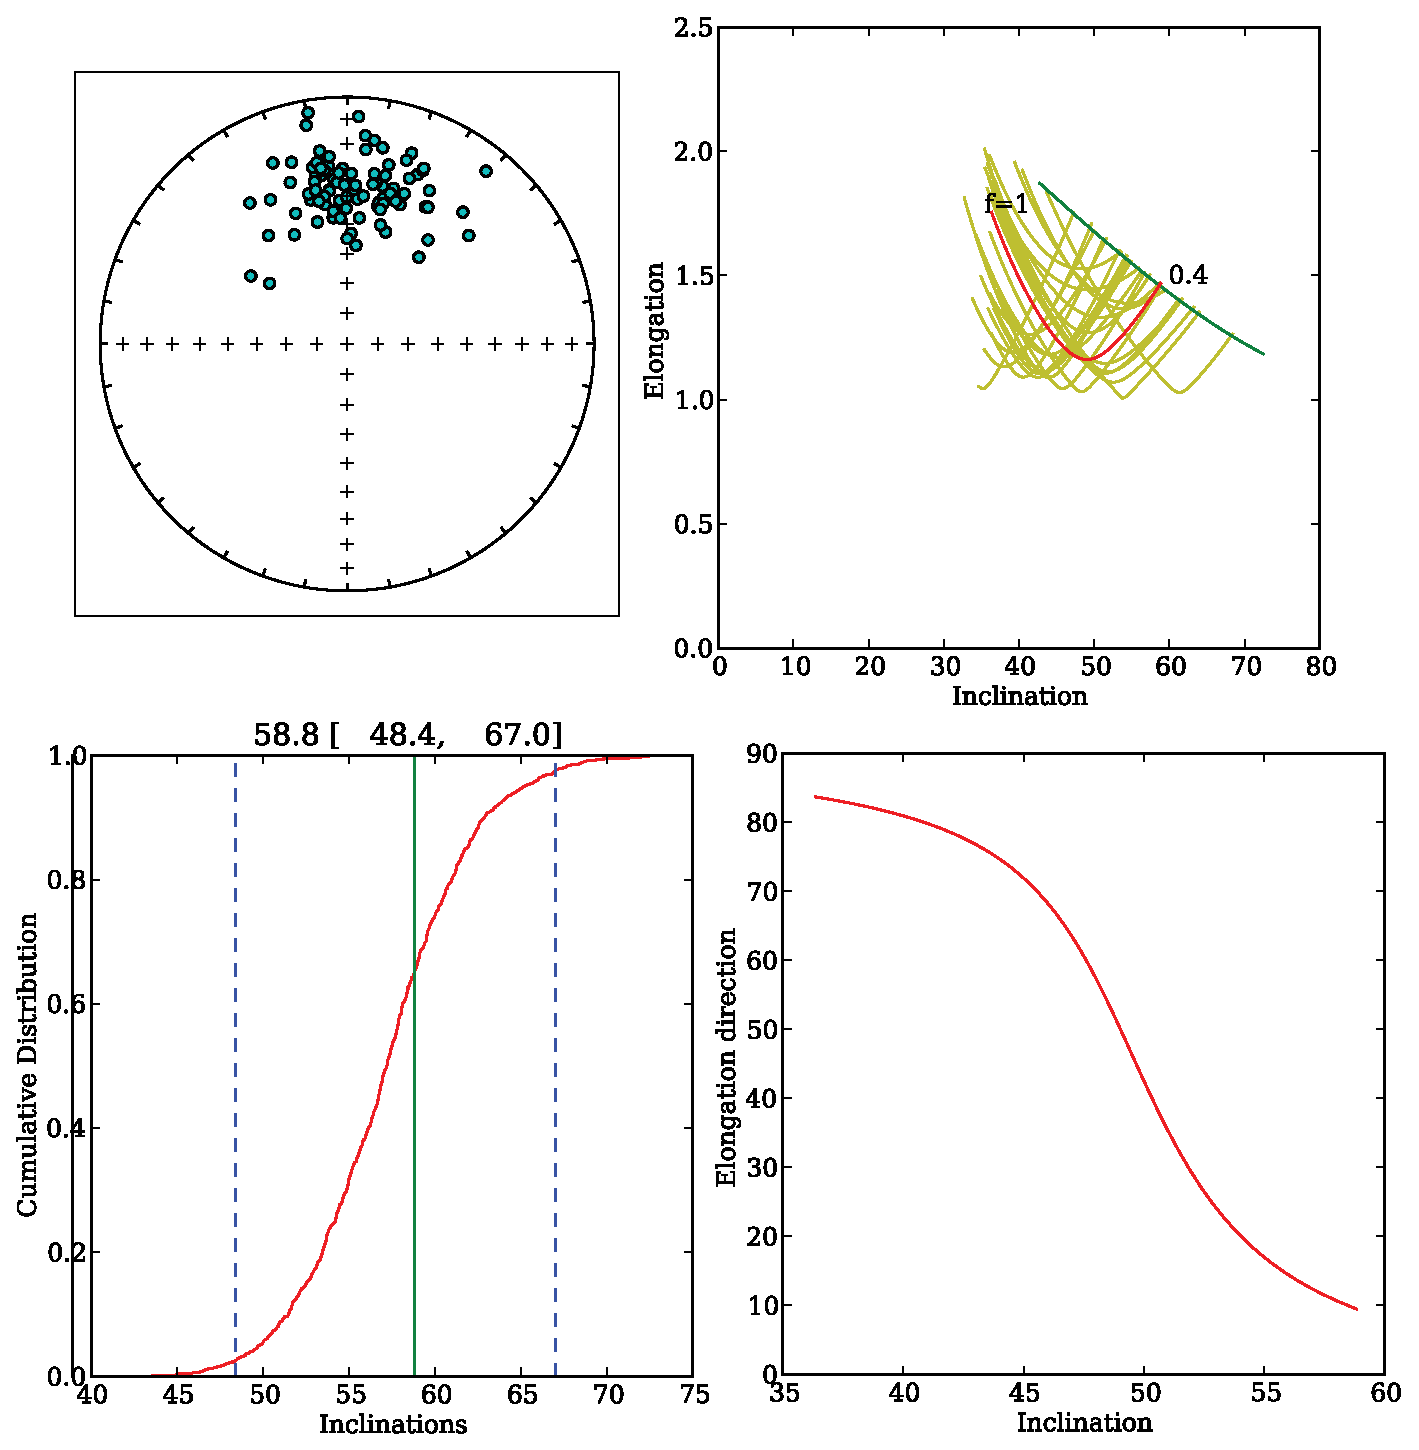
\includegraphics[width= 15 cm]{EPSfiles/find_EI.eps}

In this example, the original expected inclination at paleolatitude of 42 (61$^{\circ}$) is recovered within the 95\% confidence bounds.  

%

%\customlink{fisher.py}
\section {\bf fisher.py}
\href{http://Webbook2.html#Fisher_statistics}{ [Chapter 11]}

Draw a set of 10 directions from a Fisher distribution with a $\kappa$ of 30 using {\bf fisher.py}:

\begin{verbatim}
% fisher.py -k 30 -n 10
  233.7    81.4 
  357.0    76.4 
  272.5    62.8 
  137.0    70.0 
   83.7    71.2 
...
  \end{verbatim}
  
  You could plot the output with, e.g., \href{#eqarea.py}{eqarea.py}.  
  
  Note that every instance of this program draws a different distribution, so yours will look different in detail.  


%\customlink{fishqq.py}
\section {\bf fishqq.py} 
\href{http://Webbook2.html#Fisher_statistics}{ [Chapter 11]}

Test whether a set of 100 data points generated with \href{#fisher.py}{fisher.py} are in fact Fisher distributed by using a Quantile-Quantile plot:

\begin{verbatim}
% fisher.py -k 30 -n 100 >fishqq_example.txt
% fishqq.py -f fishqq_example.txt 
\end{verbatim}

\noindent produces these plots:



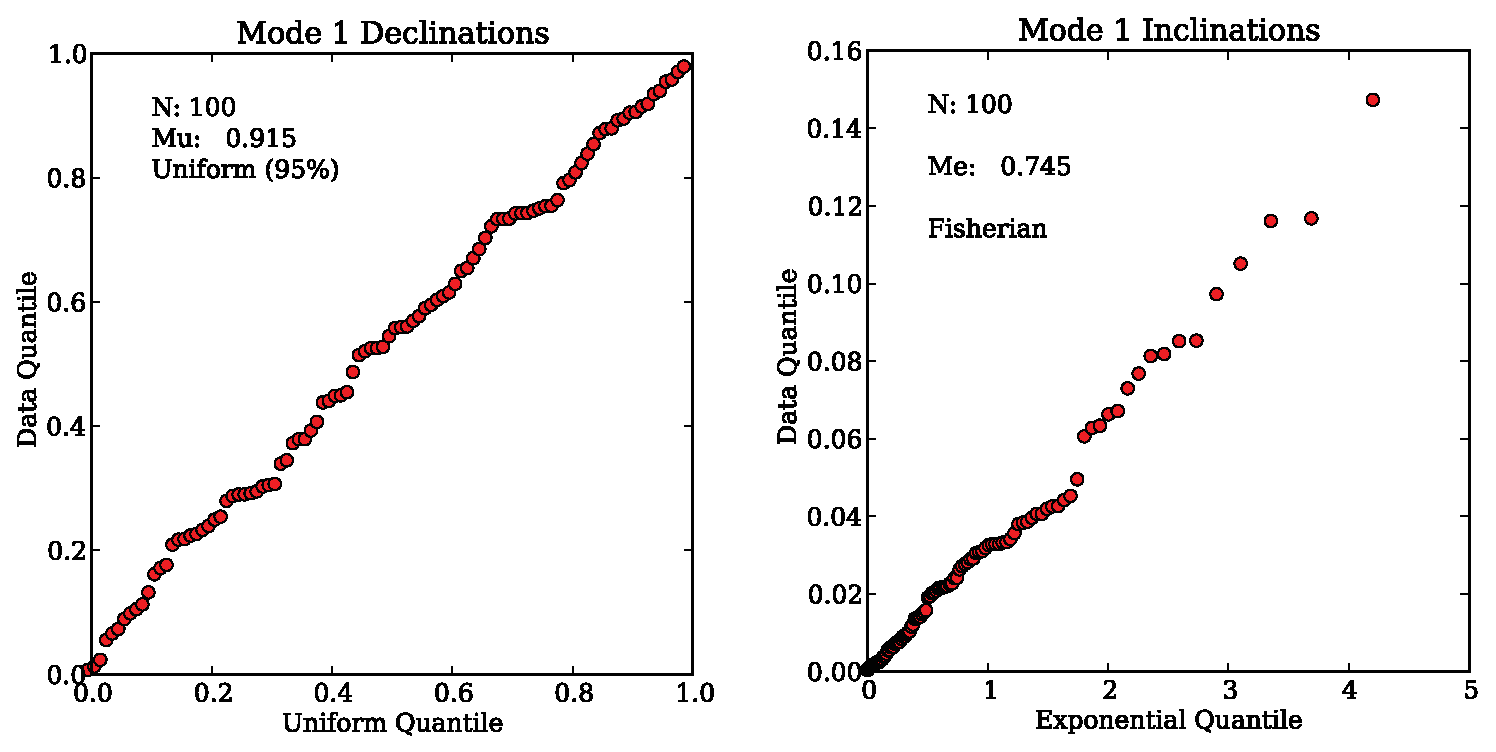
\includegraphics[width=15cm]{EPSfiles/fishqq-ex.eps}

\noindent which support a Fisher distribution for these data.  



%\customlink{fishrot.py}
\section {\bf fishrot.py} 
\href{http://Webbook2.html#Fisher_statistics}{ [Chapter 11]}

Draw a set of 5 directions drawn  from a Fisher distribution with a true mean declination of 33, a true mean inclination of 41, and a $\kappa$ of  50:

\begin{verbatim}
% fishrot.py -n 5 -D 33 -I 41 -k 50
   35.8    32.8 
   36.2    30.2 
   37.5    41.8 
   28.6    23.9 
   26.1    32.8 
   \end{verbatim}

%\customlink{foldtest.py}
 \section {\bf foldtest.py}
 \href{http://Webbook2.html#Beyond_Fisher_statistics}{[Chapter 12]}

 Use {\bf foldtest.py} to perform a foldtest on the data in {\it foldtest\_example.dat}.   
 
 \begin{verbatim}
% foldtest.py -f foldtest_example.dat 
doing  1000  iterations...please be patient.....
0
50
100
.
.
.

82 - 117 Percent Unfolding
range of all bootstrap samples:  70  -  137
S[a]ve all figures, <Return> to quit   a
3  saved in  fold_ta.svg
2  saved in  fold_st.svg
1  saved in  fold_ge.svg
 \end{verbatim}
 
\noindent  which gives the plots:
 
 %\epsfxsize 14cm
 {%\epsffile{EPSfiles/foldtest-ex.eps}
   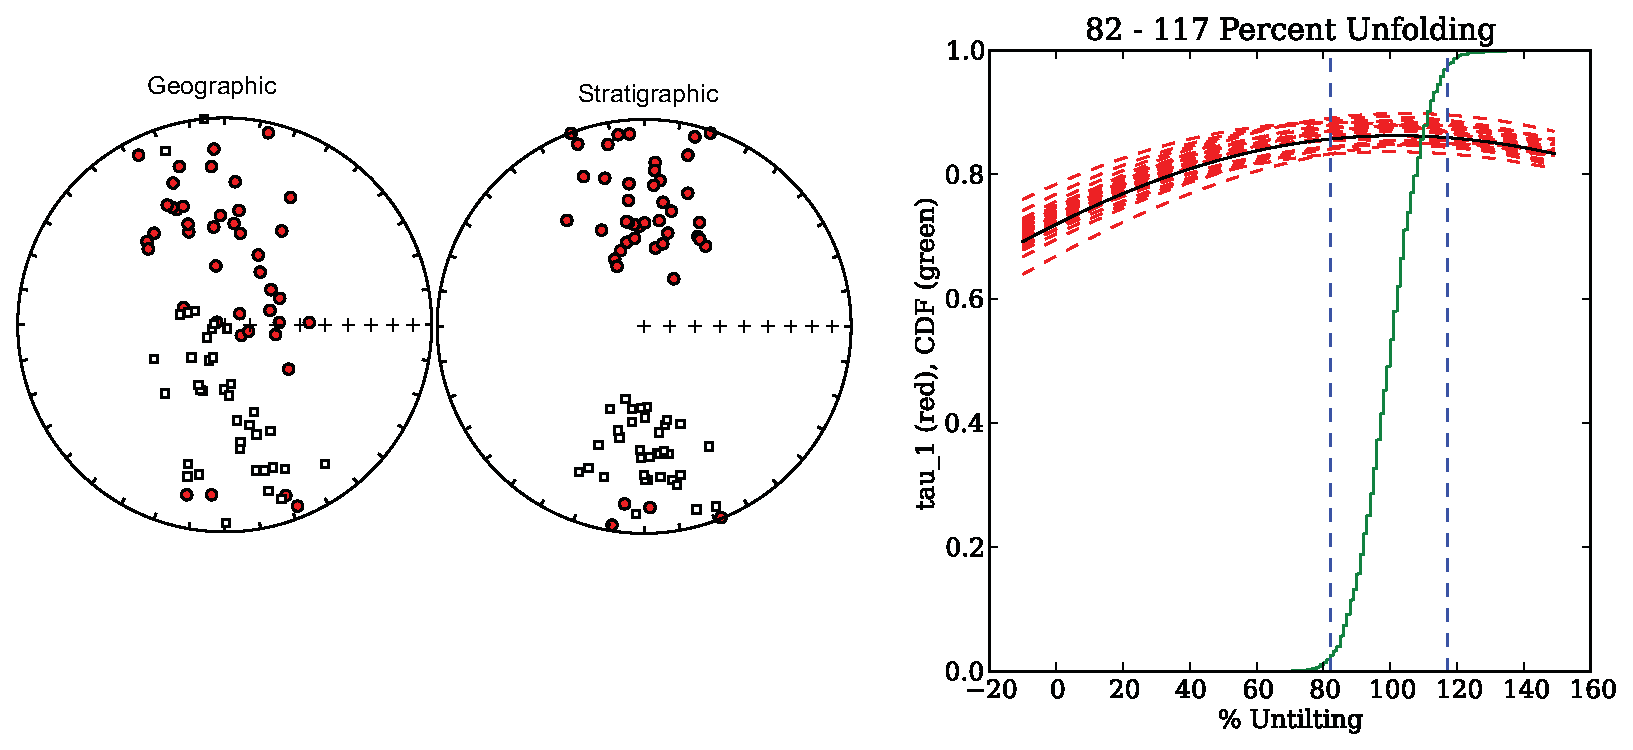
\includegraphics[width=14 cm]{EPSfiles/foldtest-ex.eps}}
 
 Apparently these directions were acquired prior to folding because the 95\% confidence bounds on the degree of untilting required for maximizing concentration of the data (maximum in principle eigenvalue) $\tau_1$ of orientation matrix (see the section on  \href{Webbook2.html#orientation_tensor}{eigenvalues} in the textbook) includes 100\%.  
% 
% 
%\customlink{foldtest_magic.py}
\section{foldtest\_magic.py} \href{http://Webbook2.html#Beyond_Fisher_statistics}{[Chapter 12]} and \href{#MagIC}{[MagIC]}

This program performs the same test as \href{#foldtest.py}{foldtest.py}.  The only difference is that it reads MagIC formatted input files and allows the application of selection criteria as specified in the {\it pmag\_criteria.txt} formatted file.   
% 
% 
%\customlink{gaussian.py}
\section{gaussian.py} 
 \href{http://Webbook2.html#Fisher_statistics}{[Chapter 11]}

Use {\bf gaussian.py} to generate a set of 100 normally distributed data points drawn from a population with a mean of 10.0  and   standard deviation of 30.  Save it to a file named {\bf gauss.out}.  

\begin{verbatim}
% gaussian.py -s 3 -n 100 -m 10. -F gauss.out
\end{verbatim}

You can check the sample mean and standard deviation with \href{#stats.py}{stats.py} or make a histogram of the data with\href{#hisplot.py}{histplot.py}




%\customlink{gobing.py}
\section {\bf gobing.py}
 \href{http://Webbook2.html#Beyond_Fisher_statistics}{[Chapter 12]}

Use the dataset generated in the \href{#eqarea_ell.py}{eqarea\_ell.py} example.   Calculate Bingham parameters using {\bf gobing.py}  instead of within the plotting program:

\begin{verbatim}
% gobing.py -f tk03.out 
  357.8    60.3     4.5   105.7    10.0     4.5    21.0   -27.6 20
\end{verbatim}

\noindent  which according to the help message from {\bf gobing.py} is:  

mean dec, mean inc, Eta, Deta, Ieta, Zeta, Zdec, Zinc, N


%\customlink{gofish.py}
\section {\bf gofish.py} 
 \href{http://Webbook2.html#Fisher_statistics}{[Chapter 11]}
 
 Draw a set of 10 directions drawn  from a Fisher distribution with a true mean declination of 15, a true mean inclination of 41, and a $\kappa$ of  50 and save it to a file, then use {\bf gofish.py} to calculate the Fisher parameters:

\begin{verbatim}
%  fishrot.py -n 10 -D 15 -I 41 -k 50 >fishrot.out
% gofish.py -f  fishrot.out 
   10.8    39.6    10     9.8484     59.4     6.3    10.5
   \end{verbatim}
   
\noindent     which according to the help message from {\bf gofish.py -h} is:   mean dec, mean inc, N, R, k, a95, csd.  Your results will vary because every instance of \href{#fishrot.py}{fishrot.py} draws a different sample from the Fisher distribution.   

%

%\customlink{gokent.py}
\section {\bf gokent.py} 
 \href{http://Webbook2.html#Beyond_Fisher_statistics}{[Chapter 12]}

Draw a set of 20 data points  from a TK03.GAD distibution predicted for a latitude of 42$^{\circ}$N (see  14), without  reversals.  Calculate kent parameters using {\bf gokent.py} 

\begin{verbatim}
% tk03.py -n 20 -lat 42 >tk03.out; gokent.py -f  tk03.out
   359.2    55.0     9.3   147.7    30.8     7.8   246.8    14.9 20
\end{verbatim}

\noindent  which according to the help message from {\bf gobing.py} is:   mean dec, mean inc, Eta, Deta, Ieta, Zeta, Zdec, Zinc, N


\section {\bf goprinc.py} [Chapter 12]
 \href{http://Webbook2.html#Beyond_Fisher_statistics}{[Chapter 12]}

Draw a set of 20 data points  from a TK03.GAD distibution predicted for a latitude of 42$^{\circ}$N (see  14), including reversals.  Calculate the eigenparameters of the orientation matrix (the principal components)  using {\bf goprinc.py} 

\begin{verbatim}
% tk03.py -n 20 -lat 42 -rev >tk03.out; goprinc.py -f tk03.out
0.93863    11.0    58.6 0.04258   226.4    26.5 0.01879   128.3    15.6 20
\end{verbatim}

\noindent  which according to the help message from {\bf gobing.py} is:    $\tau_1 V1_D, V1_I,  \tau_2 V2_D V2_I \tau_3 V3_D V3_I, N$.

%\customlink{grab_magic_key.py}
\section{grab_magic_key.py}
\href{#MagIC}{[MagIC]}

{\bf grab\_magic\_key.py} is  a utility that will print out any column (-key option) from any \href{#MagIC}{[MagIC]} formatted file.  For example, we could print out all the site latitudes from the  {\it er\_sites.txt} file down loaded in the \href{#download_magic.py}{download\_magic.py} example:

\begin{verbatim}
% grab_magic_key.py -f er_sites.txt -key site_lat
42.60264
42.60264
42.60352
42.60104
...
\end{verbatim}

You could save the data in a file with the output redirect function ($>$ ) and plot them with, say \href{#plot_cdf.py}{plot\_cdf.py}.  

\begin{verbatim}
% grab_magic_key.py -f er_sites.txt -key site_lat > lats 
% plot_cdf.py -f lats
\end{verbatim}

which produces  the fascination (NOT!) plot:

\includeraphics[width=10cm]{grab_magic_key.eps}


%\customlink{histplot.py}
\section {\bf histplot.py}

Make a histogram of the data generated with the {\bf gaussian.py} program.



\begin{verbatim}
% histplot.py -f gauss.out
\end{verbatim}

\noindent  which makes a plot similar to:

  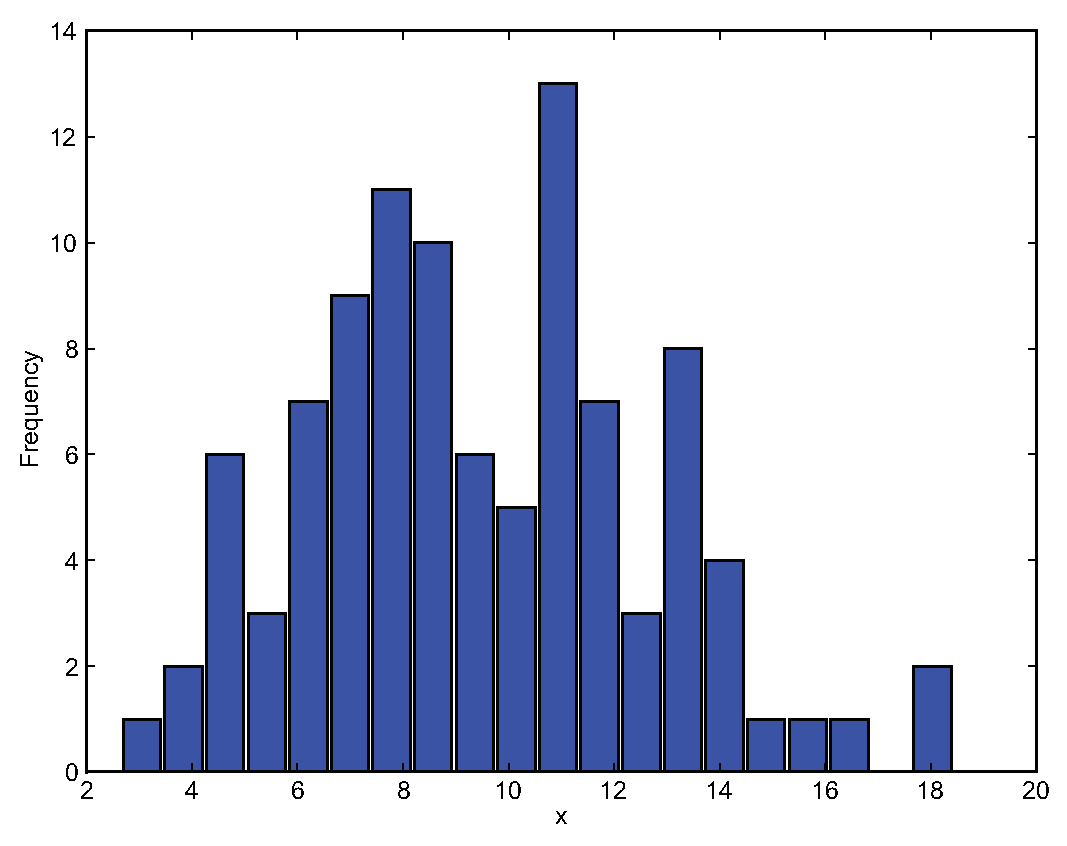
\includegraphics[width=10 cm]{EPSfiles/hist.eps}

%\customlink{hysteresis_magic.py}
\section {\bf hysteresis\_magic.py} [Chapters 5, 7  \& Appendices~\ref{app:hyst}, ~\ref{app:MagIC}]

Plot the magic\_measurements formatted hysteresis experimental data  created by \newline {\bf agm\_magic.py}.   Use the program  {\bf hysteresis\_magic.py}.   

\begin{verbatim}
% hysteresis_magic.py -f hysteresis_magic_example.dat

IS06a-1 1 out of  8
S[a]ve plots, [s]pecimen name, [q]uit, <return> to continue
 a
1  saved in  _IS06a-1_hyst.svg
3  saved in  _IS06a-1_DdeltaM.svg
2  saved in  _IS06a-1_deltaM.svg
5  saved in  _IS06a-1_irm.svg
\end{verbatim}

\noindent which makes the plots:


  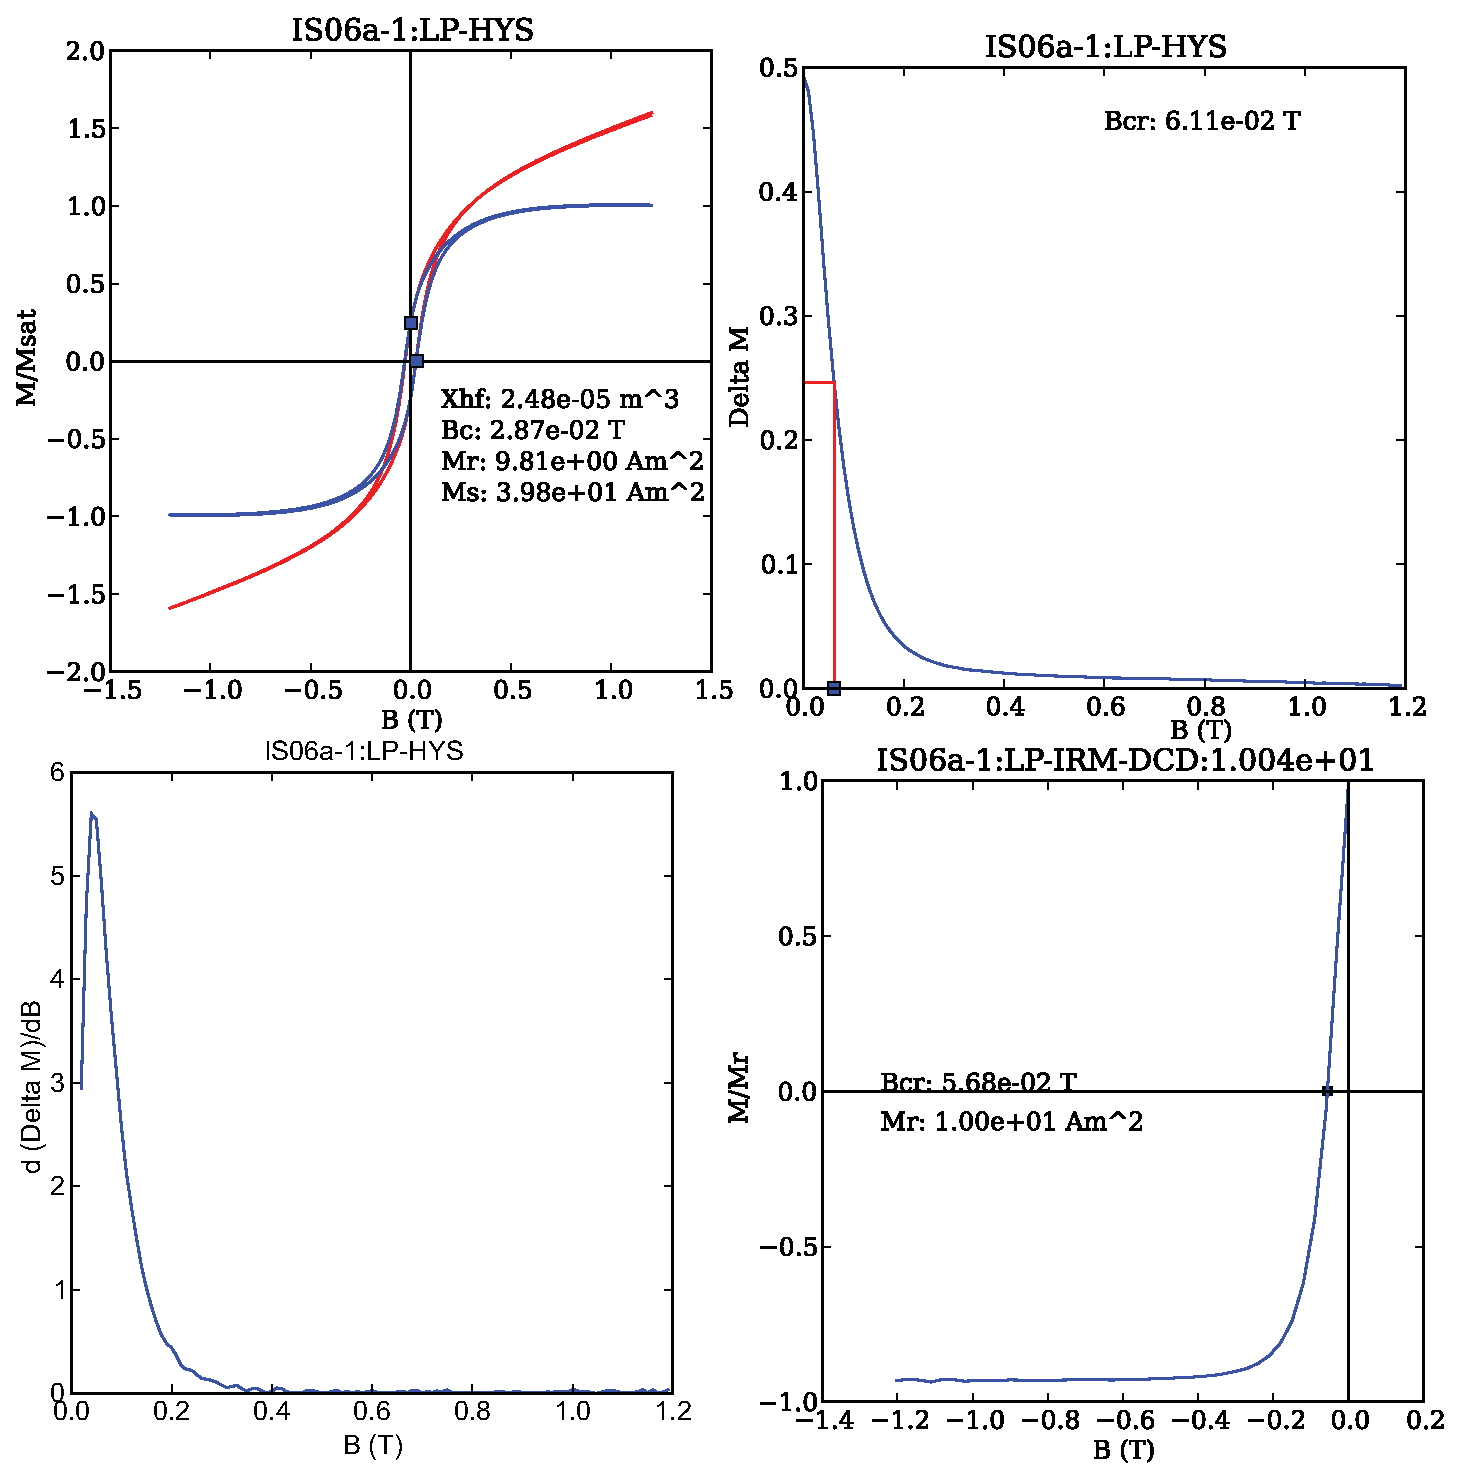
\includegraphics[width=20 cm]{EPSfiles/hysteresis-magic.eps}




%\customlink{igrf.py}
\section {\bf igrf.py} 
\href{http://Webbookcopy.html#The_geomagnetic_field}{[Chapter 2]}[Chapter 2]


Use the program {\bf igrf.py } to estimate the
field on June 1, 1995 in Amsterdam, The Netherlands (52.5$^{\circ}$ N, 5$^{\circ}$E).

\begin{verbatim}
% igrf.py -i
Decimal year: <cntrl-D to quit> 1995.5
Elevation in km [0] 
Latitude (positive north) 52.5
Longitude (positive east) 5
  357.9    67.4    48534
  
Decimal year: <cntrl-D to quit> ^D
 Good-bye
\end{verbatim}

Now read from the file {\it igrf\_example.dat} which requests field information for near San Diego for the past 3000 years.  The program will evaluate the field vector for that location for dates from 1900 to the present using the IGRF/DGRF coefficients in the IGRF-11 model available from:
\url{http://www.ngdc.noaa.gov/IAGA/vmod/igrf.html}.   For the period from 1000 BCE to 1800, the program uses the CALS3k.4b of Korte and Constable (2011).  \nocite{korte11a} available at: \url{http://earthref.org/ERDA/1142/}.    Prior to that and back to 8000 BCE, the program uses the coefficients of Korte et al., 2011 \nocite{korte11b} for the CALS10k.1b, available at:
\url{http://earthref.org/ERDA/1403/}

\begin{verbatim}
% igrf.py -f igrf_example.dat -F igrf.out
\end{verbatim}

You can plot the output using, for example \href{#plotXY.py}{plotXY.py}:  

\begin{verbatim}
% igrf.py -f igrf_example.dat -F igrf.out
% plotXY.py -f igrf.out -c 2 4 -l -xlab Inclination -ylab Year
S[a]ve to save figure, <Return>  to quit  a
Figure saved as:  plotXY.svg
\end{verbatim}

which produces a plot like this:  
  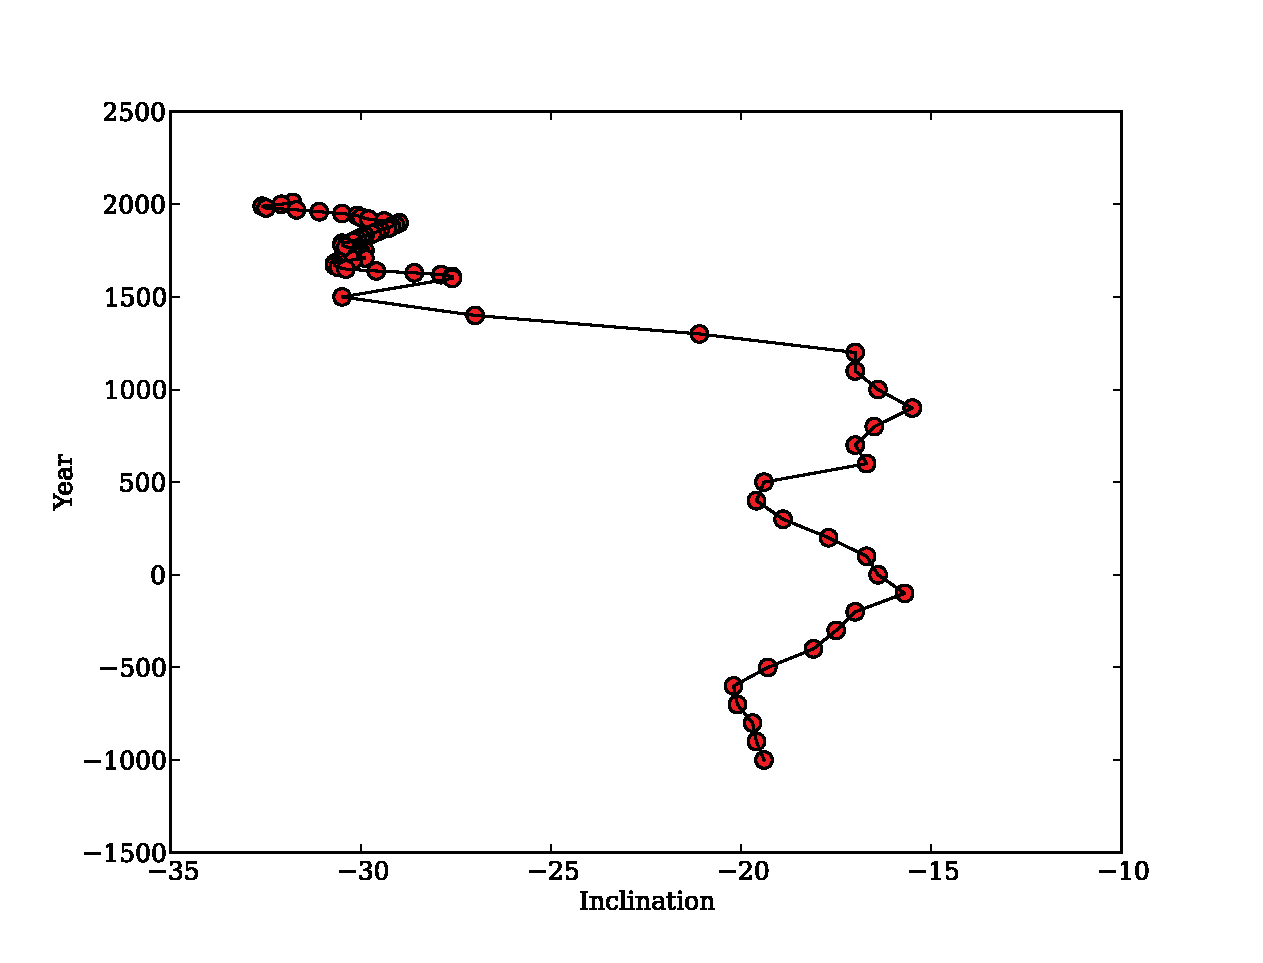
\includegraphics[width=15 cm]{EPSfiles/plotXY.eps}


%\customlink{incfish.py}
\section {\bf incfish.py}
\href{http://Webbook2.html#Fisher_statistics}{ [ Chapter 11]}

Use the program {\bf incfish.py} to calculate average inclination for inclination only data 
simulated by fishrot.py for an average inclination of 60$^{\circ}$.   If you save the declination, inclination 
pairs, you can compare the {\bf incfish.py} answer with the Fisher mean.    The datafile {\it incfish\_example\_di.dat} has the declination, inclination pairs and {\it incfish\_example\_inc.dat} has just the inclinations.  

\begin{verbatim}
% fishrot.py -I 60 -k 10 > incfish_example_di.dat
% awk '{print $2}' incfish_example_di.dat > incfish_example_inc.dat
% incfish.py -f incfish_example_inc.dat 
   57.1    61.0  100     92.9    13.9     1.0
% gofish.py -f incfish_example_di.dat 
    1.8    62.9    100    91.2727     11.3     4.4    24.0
\end{verbatim}

The output for {\bf incfish.py} is:  [gaussian] mean inc, Fisher inc, $N, R, k, \alpha_{95}$.  You can see that the {\bf incfish.py} result is much closer to the Fisherian result than the gaussian mean is. 

%\customlink{irmaq_magic.py}
\section{irmaq\_magic.py}
\href{#MagIC}{MagIC}

Someone (Saiko Sugisaki) measured a number of samples from IODP Expedition 318 Hole U1359A for IRM acquisition curves.  She used the ASC impulse magnetizer's coils \# 2 and 3 and saved the data in the \href{#sio_magic.py}{SIO format}.   Convert these to the {\it \href{#MagIC}{MagIC} measurements  format, combine them in a  single {\it magic\_measurements.txt} file with \href{#combine_magic.py}{combine\_magic.py} and plot the data with {\bf irmaq\_magic.py}. 

\begin{verbatim}
% sio_magic.py -f U1359A_IRM_coil2.txt -LP I -V 2 -F U1359A_IRM_coil2.magic -loc U1359A
% sio_magic.py -f U1359A_IRM_coil3.txt -LP I -V 3 -F U1359A_IRM_coil3.magic -loc U1359A
% combine_magic.py -F magic_measurements.txt -f U1359A_IRM_coil2.magic U1359A_IRM_coil3.magic
% irmaq_magic.py
559  records read from  magic_measurements.txt
U1359A
 S[a]ve to save plot, [q]uit,  Return to continue:  a
1  saved in  U1359A_LP-IRM.svg
\end{verbatim}

which produces the plot:

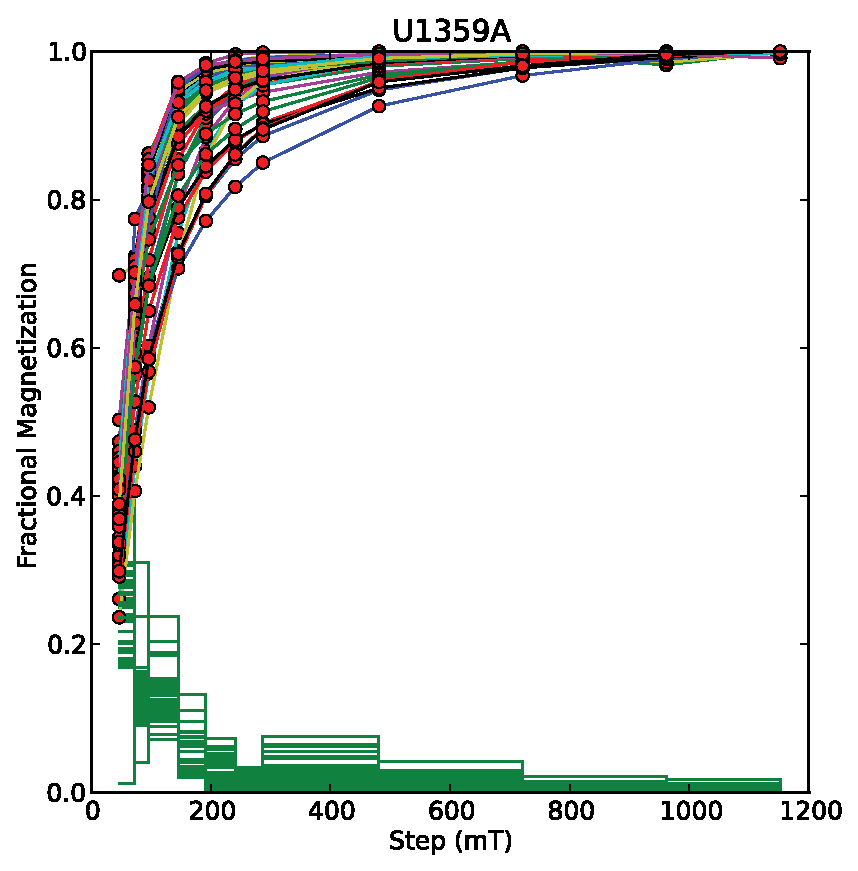
\includegraphics[width=10cm]{EPSfiles/irmaq_magic.eps}

%
%\customlink{k15_magic.py}
\section {\bf k15\_magic.py} 
[\href{http://magician.ucsd.edu/Essentials/WebBook2.html#Paleomagnetic_tensors}{Chapter 13}; 
\href{#MagIC}{[MagIC]}


Someone took a set of samples from a dike margin in the Troodos Ophiolite and measured their anisotropy of magnetic susceptibility on an a Kappabridge KLY 2.0 instrument in the SIO laboratory.  The sequence of measurement positions is that recommended by Jelinek (1977):  \nocite{jelinek77}

  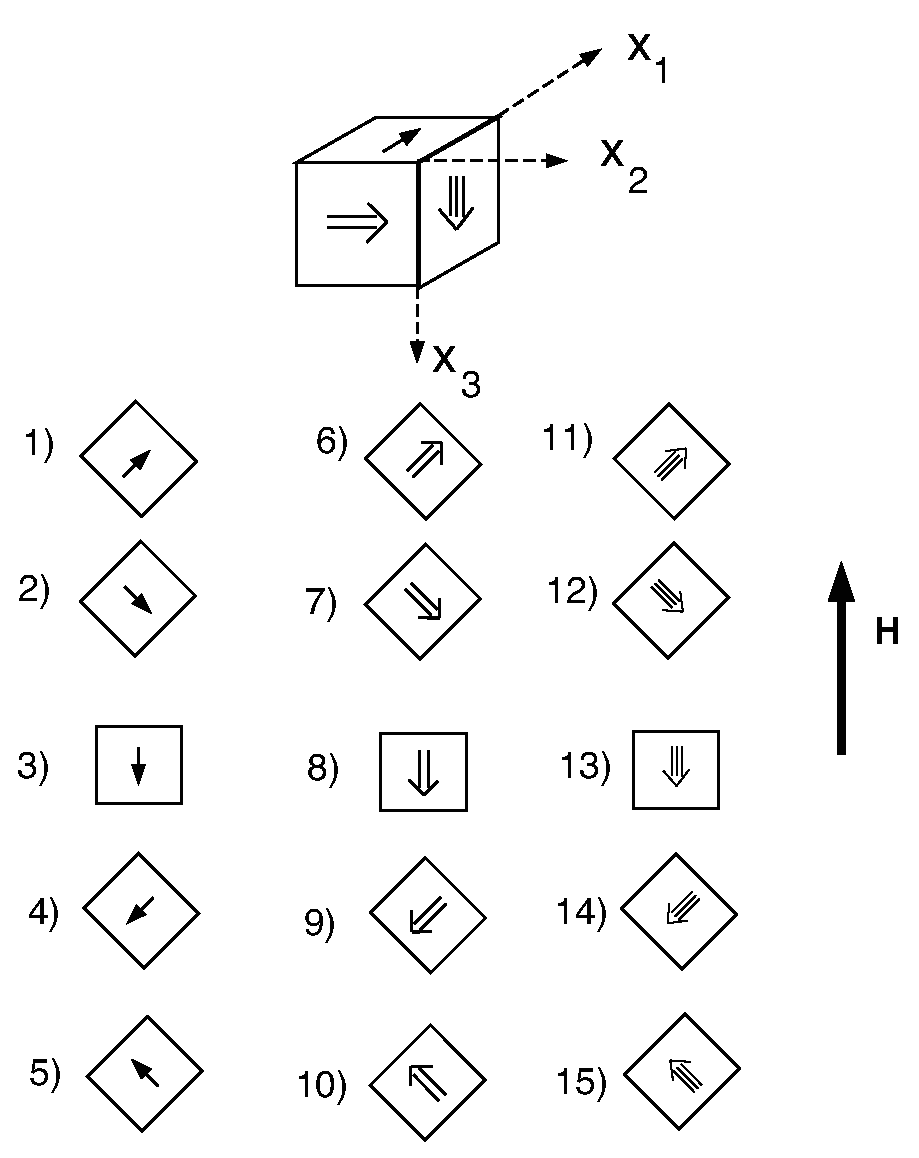
\includegraphics[width=15 cm]{EPSfiles/meas15.eps}
  
  
  The 15 measurements for each specimen, along with orientation information and the specimen name were saved in the file {\it k15\_example.dat}.    Convert these to the MagIC format using the program {\bf k15\_magic.py}:

\begin{verbatim}
% k15_magic.py -spc 0 -f k15_example.dat -loc "Troodos Ophiolite"
Data saved to:  ./er_samples.txt ./rmag_anisotropy.txt ./rmag_results.txt ./k15_measurements.txt
 \end{verbatim}

You can plot the output of this example (default file {\it rmag\_anisotropy.txt}) using the program {\bf aniso\_magic.py}.     

%\customlink{k15_s.py}
\section {\bf k15\_s.py}  
[\href{http://magician.ucsd.edu/Essentials/WebBook2.html#Paleomagnetic_tensors}{Chapter 13}; 
\href{#MagIC}{[MagIC]}

%
Use {\bf k15\_s.py} to calculate the best-fit tensor elements and residual error for the data in the file {\it k15\_example.dat} (same file as for \href{#k15_magic.py}{k15_magic.py}.  These are: the specimen name, azimuth and plunge and the strike and dip, followed by the 15 measurements made using the Jelinek 1977 \nocite{jelinek77} scheme shown in the \href{#k15_magic.py}{k15_magic.py} example.  Calculate the .s data in specimen, geographic  and tilt adjusted coordinates:

\begin{verbatim}
% k15_s.py -f k15_example.dat
0.33146986 0.33413991 0.33439023 0.00075095 -0.00083439 -0.00016688 0.00008618
0.33335925 0.33335925 0.33328149 -0.00155521 -0.00132193 0.00116641 0.00017193
0.33097634 0.33573565 0.33328801 0.00163177 0.00013598 0.00000000 0.00018131
...
% k15_s.py -f k15_example.dat -crd g
0.33412680 0.33282733 0.33304587 -0.00015289 0.00124840 0.00135721 0.00008618
0.33556300 0.33198264 0.33245432 0.00087259 0.00024141 0.00096166 0.00017193
0.33584908 0.33140627 0.33274469 0.00131844 0.00118816 0.00002987 0.00018131
...
% k15_s.py -f k15_example.dat -crd t
0.33455712 0.33192658 0.33351630 -0.00043563 0.00092770 0.00105006 0.00008618
0.33585501 0.33191562 0.33222935 0.00055960 -0.00005314 0.00064730 0.00017193
0.33586666 0.33084926 0.33328408 0.00142269 0.00013235 0.00009201 0.00018131
...
\end{verbatim}

%

%\customlink{kly-asc_magic.py}
\section {\bf kly-asc\_magic.py} 
[\href{http://magician.ucsd.edu/Essentials/WebBook2.html#Paleomagnetic_tensors}{Chapter 13}; 
\href{#MagIC}{[MagIC]}


Some of the AGICO  magnetic susceptibility instrument software versions (e.g., SUFAR ver.1.2)  save data in an ascii file like that in:

 {\it kly-asc\_magic\_example.txt}.  
 
 These can be imported into the MagIC format using the program {\bf kly-asc\_magic.py} as follows:

\begin{verbatim}
% kly-asc_magic.py -f kly-asc_magic_example.dat 
anisotropy tensors put in  rmag_anisotropy.txt
anisotropy results put in  rmag_results.txt
specimen info put in  er_specimens.txt
sample info put in  er_samples.txt
site info put in  er_sites.txt    
\end{verbatim}

This command will create  a number of files needed by the MagIC database; these can be plotted using {\bf aniso\_magic.py} or imported into the MagIC console for further editing.  

%\customlink{kly4s_magic.py} 
\section {\bf kly4s\_magic.py}[\href{http://magician.ucsd.edu/Essentials/WebBook2.html#Paleomagnetic_tensors}{Chapter 13}; 
\href{#MagIC}{[MagIC]}


The program {\bf AMSSpin} available for downloading from \url{http://earthref.org/ERDA/940/}  generates data for the Kappabridge KLY4S spinning magnetic susceptibility instrument as described by Gee et al. (2008).  \nocite{gee08}  Output files are in the format of the file {\it kly4s\_magic\_example.dat}.  One option is for orientation information to be output as an {\it azdip} formatted file (see \href{#azdip_magic.py}{azdip\_magic.py}.)   
The AMS data files can be imported into the MagIC format with {\bf kly4s\_magic.py} as follows: 

\begin{verbatim}
%kly4s_magic.py -f kly4s_magic_example.dat -fad kly4s_example.azdip
\end{verbatim}

This command will create a number of files needed by the MagIC database and the data can be plotted using {\bf aniso\_magic.py}.  

%\customlink{lnp_magic.py}
\section {\bf lnp\_magic.py}
\href{http://Webbook2.html#Fisher_statistics}{ [Chapter 11},  \href{http://Webbook2.html#linesNplanes}{Appendix C2.2} \& \href{#MagIC}{MagIC}

This program will take {\it pmag\_specimen} formatted MagIC files (for example, generated by \href{#zeq_magic.py}{zeq\_magic.py}) and plot data by site, combining best-fit lines and best-fit planes using the method described in  \href{http://Webbook2.html#linesNplanes}{Appendix C2.2}.  Try this out on the data from the San Francisco Volcanics, notorious for lightning strikes, published by Tauxe et al., 2003. \nocite{tauxe03}  These can be downloaded from the MagIC database from \url{http://earthref.org/MAGIC/m000629dt20061213090720/} and unpacked with 
\href{#download_magic.py}{download\_magic.py}.   


\begin{verbatim}
% download_magic.py -f zmab0001193tmp02.txt
working on:  'er_locations'
er_locations  data put in  ./er_locations.txt
working on:  'er_sites'
er_sites  data put in  ./er_sites.txt
working on:  'er_samples'
er_samples  data put in  ./er_samples.txt
...
% lnp_magic.py -f pmag_specimens.txt -crd g
sv01
Site lines planes  kappa   a95   dec   inc
sv01 0  5     286      6.6    179.0    -54.3  4.9948 
% tilt correction:  0
s[a]ve plot, [q]uit, <return> to continue:
 a
1  saved in  sv01_g_eqarea.svg
 
\end{verbatim}

\noindent which generated this figure:

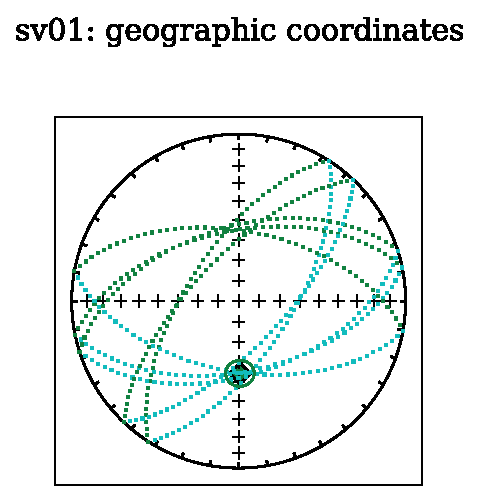
\includegraphics[width=10cm]{EPSfiles/lnp-ex.eps}}

%\customlink{lowrie.py}
\section{lowrie.py}
\href{http://Webbook2.html#lowrie}{[Chapter 8]}

Someone (Saiko Sugisaki} subjected a number of specimens from IODP Expedition 318 Hole U1359A specimens to a 3-D IRM experiment and saved the data in the \href{#sio_magic.py}{SIO} format.   
Use {\bf lowrie.py} to make plots of blocking temperature for the three  coercivity fractions.  

\begin{verbatim}

% lowrie.py -f lowrie_example.dat
318-U1359A-002H-1-W-109
S[a]ve figure? [q]uit, <return> to continue   a
1  saved in  lowrie:_318-U1359A-002H-1-W-109_.svg
318-U1359A-002H-4-W-65
S[a]ve figure? [q]uit, <return> to continue   q
\end{verbatim}

which produces plots like this:

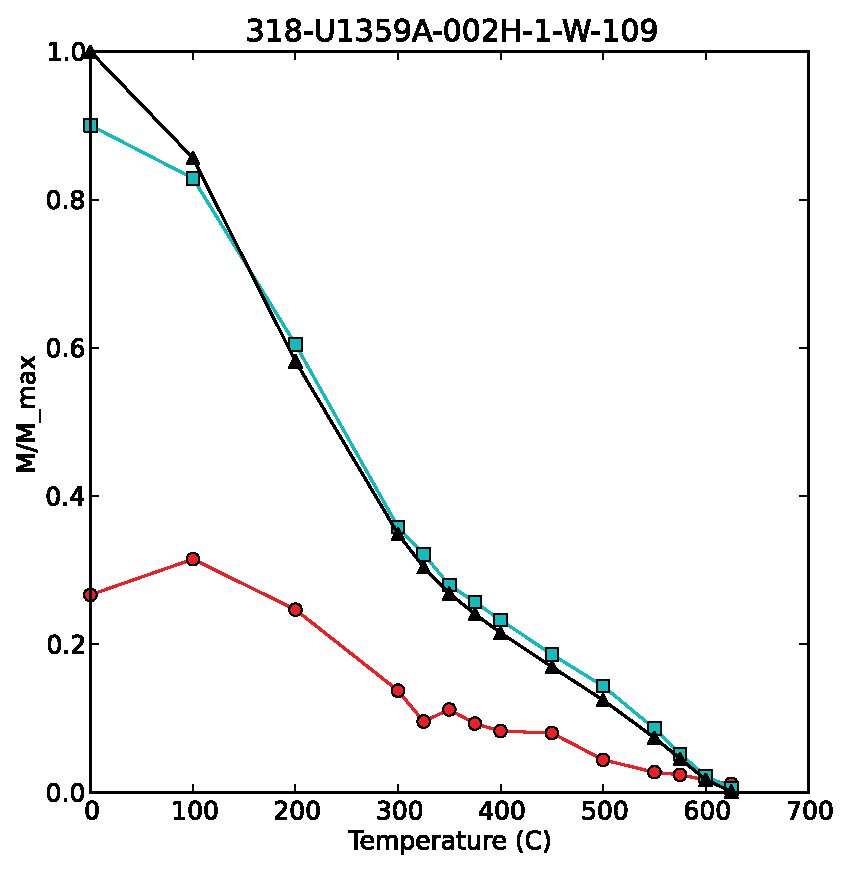
\includegraphics[width=12cm]{EPSfiles/lowrie.eps}

%\customlink{lowrie_magic.py}
\section{lowrie\_magic.py}
\href{http://Webbook2.html#lowrie}{[Chapter 8]} and \href{#MagIC}{[MagIC]}

This program works exactly like \href{#lowrie.py}{lowrie.py}, but works on {\it magic\_measurements.txt} formatted files.  Use \href{#sio_magic.py}{sio\_magic.py} to import the {\it lowrie\_example.dat} data file into the MagIC format.  Then use {\bf lowrie\_magic.py} to plot the data:

\begin{verbatim}
% sio_magic.py -f lowrie_example.dat -LP I3d -loc U1359A -F lowrie_magic_example.dat
averaging: records  11 12
318-U1359A-004H-2-W-18 started with  15  ending with  14
Averaged replicate measurements
averaging: records  13 14
318-U1359A-004H-2-W-44 started with  15  ending with  14
Averaged replicate measurements
averaging: records  14 16
318-U1359A-012H-5-W-70 started with  16  ending with  14
Averaged replicate measurements
averaging: records  14 15
% lowrie_magic.py -f lowrie_magic_example.dat 
318-U1359A-002H-1-W-109
S[a]ve figure? [q]uit, <return> to continue
\begin{verbatim}


% 
%%\section{microwave\_magic.py}  ADD this one eventually.

%

%\section{MagIC.py}[Appendix~\ref{app:MagIC}]

%This program is a graphical user interface (GUI) for many MagIC related functions.  It can be called from any directory (with no spaces in the path) and generates the program calls documented in this appendix.  It allows importing of many lab and instrument formats, plotting of a variety of data and doing the averaging and book-keeping required to create files ready for uploading into the MagIC Console software.  

ADD HERE

%
%\customlink{magic_select.py}
\section{magic\_select.py}
\href{#MagIC}{[MagIC]}


This program takes any \href{#MagIC}{MagIC} formatted file and selects lines that match the search criteria and saves the output as a new MagIC formatted file of the same type.  Selection criteria match whole or partial strings, avoid whole or partial strings or evaluate minimum or maximum values.    The syntax is to specify the input file with the -f option, the key you wish to search on with -key, followed by the string you wish to use as a criterion, followed with a 'T' for match exactly, 'F' avoid entirely, 'has' for matching partially and 'not for avoiding any partial match, and min, max and eval for evaluating the numerical value.  The -F option sets the output file.  

  For example, you could pick out all the records that match a certain site name string.  You could select out records with specified method codes.  You could get all records with inclinations that are positive.   
  
  Use {\bf magic_select.py} to pick out all the best-fit lines based on AF demagnetization data from the {\it pmag\_specimens.txt} file unpacked from the MagIC database in the \href{#download_magic.py}{download\_magic.py} example.
  
  \begin{verbatim}
  % magic_select.py -f pmag_specimens.txt -key magic_method_codes LP-DIR-AF has -F AF_specimens.txt
  % magic_select.py -f AF_specimens.txt -key magic_method_codes DE-BFL has -F AF_BFL_specimens.txt
69  records written to  .//AF_BFL_specimens.txt

  

%\customlink{make_magic_plots.py}
\section{make\_magic\_plots.py}


ADD SOMETHING HERE


%\customlink{measurements_normalize.py}
\section{measurements\_normalize.py}

ADD SOMETHING HERE

%\customlink{mk_redo.py}
\section{mk\_redo.py} 
\href{#MagIC}{MagIC}

The programs \href{#zeq_magic.py}{zeq\_magic.py} and \href{#thellier_magic.py}{thellier\_magic.py} make {\it pmag\_specimen} formatted files which can be used for further data reduction either by plotting or contributing to site means, etc.  Sometimes it is useful to redo the calculation, using anisotropy corrections or a change in coordinate systems, etc.  The re-doing of these specimen level calculations is handled by, for example \href{#zeq_magic_redo.py}{zeq\_magic\_redo.py} or \href{#thellier_magic_redo.py}{ thellier\_magic\_redo.py}.  These programs use {\it magic\_measurements} formatted files and perform calculations as dictated by a ``redo'' file which has the specimen name, bounds for calculation and, in the case of the demagnetization data interpretation, the type of calculation desired (best-fit lines with \href{http://earthref.org/cgi-bin/magic-s1-methods.cgi?database_name=magic&search_start=methods&category=Direction%20Estimation}{directional estimation magic method code}:{DE-BFL}, best-fit planes with those with  magic method code DE-BFP, etc.). 

 Make ``redo'' files from the existing  {\it pmag\_specimen} formatted file in the data files downloaded from the MagIC website as in {\bf download\_magic.py} and examine them as follows:

\begin{verbatim}
% mk_redo.py
% cat zeq_redo
sr01a1 DE-BFL 473 823 A 
sr01a2 DE-BFL 473 848 A 
sr01c2 DE-BFL 473 823 A 
sr01d1 DE-BFL 373 798 A 
.......
% cat thellier_redo
sr01a1 573 823 
sr01a2 573 848 
sr01c2 673 823 
sr01d1 373 823 

.....
\end{verbatim}

\noindent Note that the temperature steps are in kelvin and the AF demagnetization steps are in Tesla as required in the MagIC data base.    



%

%\customlink{nrm_specimens_magic.py}
\section {\bf nrm\_specimens\_magic.py} 
\href{#MagIC}{MagIC}

After making NRM measurements, it is frequently useful to look at the directions in equal area projection to get a ``quick look'' at the results before proceeding to step wise demagnetization.  The data in the magic\_measurements files are usually in specimen coordinates - not geographic, so we need a way to rotate the data into geographic and or stratigraphic coordinates and save them in a pmag\_specimens formatted file for plotting with {\bf eqarea\_magic.py}.   The program {\bf nrm\_specimens\_magic.py} will do this for you.  

Get into the directory you made for tshe {\bf download\_magic.py} example.   Use {\bf nrm\_specimens\_magic.py} to convert the NRM measurements in  {\it magic\_measurements.txt }   to geographic coordinates saved in a file named {\it nrm\_specimens.txt}.  The orientation data are in the file {\it er\_samples.txt}.    Then plot the specimen directions for the entire study using {\bf eqarea\_magic.py}:
 
 
 \begin{verbatim}
% nrm_specimens_magic.py -crd g
er_samples.txt  read in with  271  records
Data saved in  nrm_specimens.txt

% eqarea_magic.py -f nrm_specimens.txt
177  records read from  ./nrm_specimens.txt
All
sr01a1 SO-SUN   324.1    66.0
sr01a2 SO-SUN   325.3    62.1
sr01c2 SO-SUN   344.7    63.8
sr01d1 SO-CMD-NORTH   327.8    64.5
sr01e2 SO-SUN   333.7    67.0
...

 \end{verbatim}
 
 The first command created a file {\it nrm\_specimens.txt} and the second created an equal area projection of the NRM directions in geographic coordinates which should look like this:
 
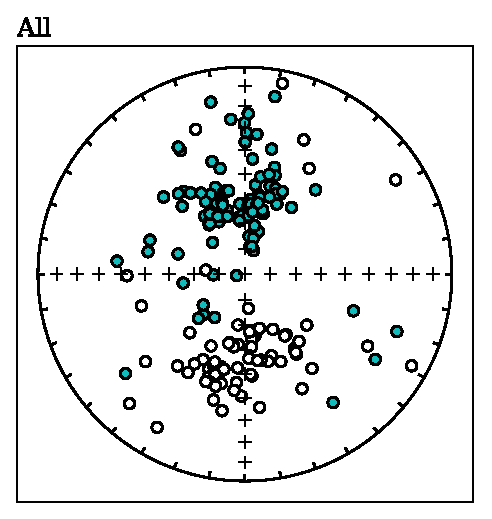
\includegraphics[width=10 cm]{EPSfiles/nrm-eq.eps}
% 

%\customlink{odp-kly4s_magic.py}
\section{odp-kly4s\_magic.py}

ADD


%\customlink{orientation_magic.py}
 \section{orientation\_magic.py}
 \href{http://Webbook2.html}{[Chapter 9]} and \href{http://earthref.org/MAGIC/help:749/#orient}{MagIC help files}
 
 There is an astounding number of different ways that paleomagnetists document data in the field and in the lab.  The MagIC database expects sample orientations to be the azimuth and plunge of the fiducial arrow used for measurement (see Chapter 9) and the orientation of the bedding to be dip direction and downward dip.  
  There are also a number of method codes that describe sampling and orientation procedures (see \url{http://earthref.org/MAGIC/methods.htm} for a complete description).  
 
 To make the conversion from notebook information to the MagIC format,  you can create a tab delimited file (orient.txt format).   This file should have all the information for a single location {\it sensu MagIC}.  A location is a stratigraphic section,  a sampling region,  an drill core, and so on.  MagIC doesn't really care what your location name is, but use the same location name every time you are asked for it, because it really ties your dataset together.   The first line of the {\it orient.txt} file should be a  header
 with the word `tab' in the first column and the desired location name in the second column.  
 
 The next row has the names of the columns .  The required columns are:  sample\_name, mag\_azimuth, field\_dip, date, lat, long, sample\_lithology, sample\_type, sample\_class) but there are a number of other possible columns (e.g., Optional Fields in orient.txt formatted files are: [date, shadow_angle, hhmm], date, stratigraphic_height, [bedding_dip_direction, bedding_dip], [image_name, image_look, image_photographer], participants, method_codes, site_name, and site_description, GPS_Az).  Nothe that column names in brackets must be supplied together and the data for stratigraphic_height are in meters. 
 
   It is handy at this point to supply the lithology, type and material classification information required by MagIC (see \href{#MagIC}{MagIC} for a brief list. Note that lithology, class and type are all controlled vocabularies listed at \url{http://earthref.org/MAGIC/shortlists.htm}.   It is also possible to put in stratigraphic height, sun compass, differential GPS orientation information, flag sample orientations as suspect, document digital field photograph names, and who was involved with the sampling.  
 
 For Sun Compass measurements, supply the shadow_angle, date and time. The date must be in mm/dd/yy format. Be sure you know the offset to Universal Time as you will have to supply that later. Also, only put data from one time zone in a single file. The shadow angle should follow the convention shown in the figure:
 
  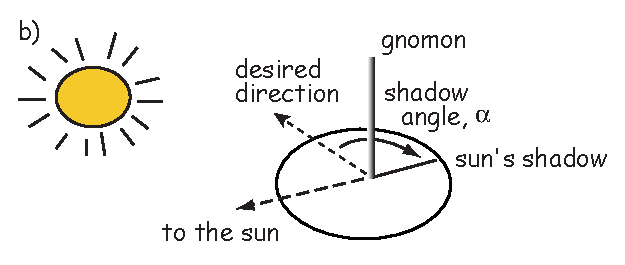
\includegraphics[width=10cm]{EPSfiles/suncomp.eps}
  
  There are options for 
 different orientation conventions (drill direction with the Pomeroy orientation device  [drill azimuth and hade] is the default), different naming conventions and a choice of whether to automatically calculate the IGRF value for magnetic declination correction, supply your own or ignore the correction.  The program generates {\it er\_samples.txt, er\_sites.txt} files.  Be warned that existing files with these names will be overwritten.   
 
 All images, for example outcrop photos are supplied as a separate zip file. image_name is the name of the picture you will import, image_look is the "look direction" and image_photographer is the person who took the picture. This information will be put in a file named er_images.txt and will ultimately be read into the er_image table in the console where addiional information must be entered (keywords, etc.).

Often, paleomagnetists note when a sample orientation is suspect in the field. To indicate that a particular sample may have an uncertainty in its orientation that is greater than about 5o, enter SO-GT5 in the method_codes column and any other special codes pertaining to a particular sample from the method codes table. Other general method codes can be entered later. Note that unlike date and sample_class, the method codes entered in orient.txt pertain only to the sample on the same line.

If there is not a supported relationship between the sample_name and the site_name (see sample naming schemes below), you can enter the site name under site_name for each sample. For example, you could group samples together that should ultimately be averaged together (multiple "sites" that sampled the same field could be grouped under a single "site name" here.


\subsection{Supported sample orientation schemes}

Samples are oriented in the field with a "field arrow" and measured in the laboratory with a "lab arrow". The lab arrow is the positive X direction of the right handed coordinate system of the specimen measurements. The lab and field arrows may not be the same. In the MagIC database, we require the orientation (azimuth and plunge) of the X direction of the measurements (lab arrow). Here are some popular conventions that convert the field arrow azimuth (mag_azimuth in the orient.txt file) and dip (field_dip in orient.txt) to the azimuth and plunge of the laboratory arrow (sample_azimuth and sample_dip in er_samples.txt). The two angles, mag_azimuth and field_dip are explained below.

[1] Standard Pomeroy convention of azimuth and hade (degrees from vertical down) of the drill direction (field arrow). sample_azimuth = mag_azimuth; sample_dip =-field_dip.

  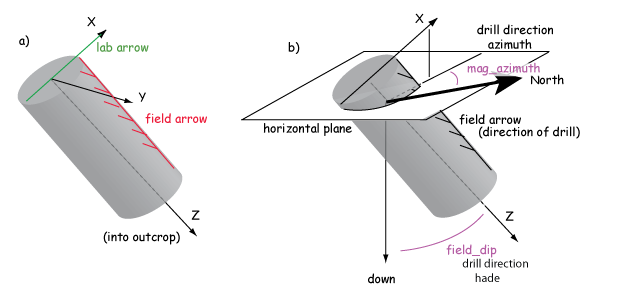
\includegraphics[width=15cm]{EPSfiles/pomeroy.png}
  
  2] Field arrow is the strike of the plane orthogonal to the drill direction, Field dip is the hade of the drill direction. Lab arrow azimuth = mag_azimuth-90o; Lab arrow dip = -field_dip
  
    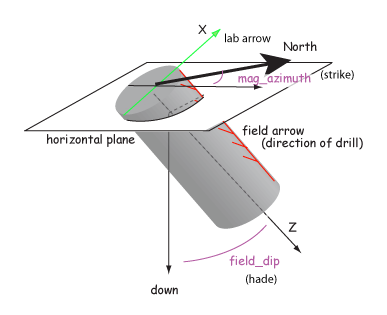
\includegraphics[width=10cm]{EPSfiles/strike_dip.png}

  [3] Lab arrow is the same as the drill direction; hade was measured in the field. Lab arrow azimuth = mag_azimuth; Lab arrow dip = 90o-field_dip.
  
      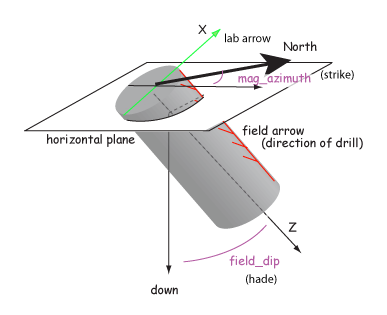
\includegraphics[width=10cm]{EPSfiles/strike_dip.png}
  
  [4] Lab arrow orientation same as mag_azimuth and field_dip.
  
        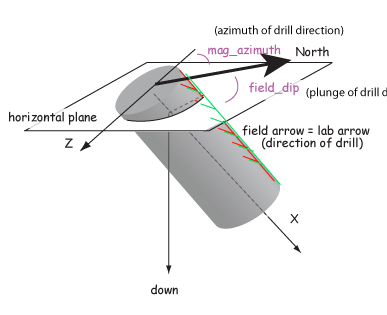
\includegraphics[width=10cm]{EPSfiles/field-lab.png}
        
        [5] Same as AZDIP convention explained below - azimuth and inclination of the drill direction are mag_azimuth and field_dip; lab arrow is as in [1] above. field arrow are lab arrow azimuth is same as mag_azimuth, Lab arrow dip = field_dip-90o
        
               \includegraphics[width=10cm]{EPSfiles/azdip.png}
               
 
 [6] Lab arrow azimuth = mag_azimuth-90o, Lab arrow dip = 90o-field_dip, i.e., field arrow was strike and dip of orthogonal face:
 
                \includegraphics[width=10cm]{EPSfiles/hand.png}           
        
        \subsection{Structural correction conventions}
        

Because of the ambiguity of strike and dip, the MagIC database uses the dip direction and dip where dip is positive from 0 $\rightarrow$ 180. Dips$ > $90 are overturned beds. 


        
\subsection{Supported sample naming schemes}

\begin{verbatim}
            [1] XXXXY: where XXXX is an arbitrary length site designation and Y
                is the single character sample designation.  e.g., TG001a is the
                first sample from site TG001.    [default]
            [2] XXXX-YY: YY sample from site XXXX (XXX, YY of arbitary length)
            [3] XXXX.YY: YY sample from site XXXX (XXX, YY of arbitary length)
            [4-Z] XXXX[YYY]:  YYY is sample designation with Z characters from site XXX
            [5] site name = sample name
            [6] site name entered in site_name column in the orient.txt format input file  
            [7-Z] [XXX]YYY:  XXX is site designation with Z characters from samples  XXXYYY
\end{verbatim}
     
  Try to import the file {\it orientation\_example.txt}.  It has field information for a few sites.  The samples were oriented with a Pomeroy orientation device  (the default) and it is desirable to calculate the magnetic declination from the IGRF at the time of sampling (also the default).  Sample names follow the rule that the sample is designated by a letter at the end of the site name (convention \#1 - which is the default).  So we do this by:
  
  \begin{verbatim}
orientation_magic.py -f orient_example.txt 
saving data...
Data saved in  ./er_samples.txt  and  ./er_sites.txt

\end{verbatim}

%
%\customlink{pca.py}
\section{pca.py} 
\href{http://Webbook2.html/#Fisher_statistics}{[Chapter 11]}

This program calculates best-fit lines, planes or Fisher averages through selected treatment steps.  The file format is 
a simple space delimited file with specimen name, treatment step,  intensity, declination and inclination.  Calculate the best-fit 
line through the first ten treatment steps in data file {\it zeq\_example.txt}:  
  
 \begin{verbatim}
 % pca.py -dir L 1 10 -f zeq_example.dat
eba24a DE-BFL
0 0.00 339.9 57.9 9.2830e-05
1 2.50 325.7 49.1 7.5820e-05
...
eba24a DE-BFL 10    2.50  70.00    8.8   334.9    51.5
\end{verbatim}
 
 According to the help message, this is: specimen name, calculation type, N, beg, end, MAD, declination and inclination.   The calculation type is the MagIC method code for best-fit lines (see Appendix~\ref{app:MagIC}.)
 

  
  %\customlink{pick_AC_specimens.py}
  \section{pick\_AC\_specimens.py}
  
  ADD
  
  %\customlink{plotXY.py}
  \section{plotXY.py}
  
  ADD
  
  %\customlink{plot_cdf.py}
  \section{plot\_cdf.py}
  
  ADD
  
  %\customlink{plot_magic_keys.py}
  \section{plot\_magic\_keys.py}
  
  ADD
  %\customlink{plotdi_a.py}
\section {\bf plotdi\_a.py} 
\href{http://Webbook2.html/#Fisher_statistics}{[Chapter 11]}

Place the following declination, inclination $\alpha_{95}$ data in a space delimited file called \newline {\it plotdi\_a\_example.dat}. 

\begin{tabular}{rrr}
\hline
Dec&Inc&$\alpha_{95}$\\
\hline
39.1 & 37.5 & 5.0\\
30.3 & 36.2 & 15\\
29.9 & 45.6 & 7\\
34.6 & 28.4 & 3\\
\hline
\end{tabular}

Make a plot of these data using {\bf plotdi\_a.py}:

\begin{verbatim}
% plotdi_a.py -f plotdi_a_example.dat
 S[a]ve to save plot, [q]uit, Return to continue:  a
1  saved in  eq.svg
\end{verbatim}
\noindent  which makes the plot:

%\epsfxsize 7cm
{\hskip 3.5cm %\epsffile{EPSfiles/plotdi-a-example.eps}
  \includegraphics[width=7 cm]{EPSfiles/plotdi-a-example.eps}}
   

%\section{pmag\_results\_extract.py} [Appendix~\ref{app:MagIC}]

%This program extracts a tab delimited txt file from a {\it pmag\_results} formatted file.   This allows you to publish data tables that have identical data to the data uploaded into the MagIC database.    Try this out in the directory created for the {\bf download\_magic.py} example:

%\begin{verbatim}
%% pmag_results_extract.py -f pmag_results.txt 
%data saved in intensites.txt and/or directions.txt
%\end{verbatim}

%This creates tab delimited files that can be incorporated into a paper, for example.

%

%\section{qqlot.py} [Appendix~\ref{app:qq}]

%Makes a quantile-quantile plot (see Appendix~\ref{app:qq}) of the input data file against a normal distribution.  
%The plot has the mean, standard deviation and the $D$ statistic as well as the $D_c$ statistic expected from 
%a normal distribution.  Use {\bf qqplot.py} to test whether the data generated with {\bf gaussian.py} is in fact normally distributed.
%(It will be 95\% of the time!).  

%\begin{verbatim}
%% gaussian.py  -F  gauss.out
%% qqplot.py -f gauss.out
%mean,sigma, d, Dc
%0.02069909 0.849042146783 0.0528626896977 0.0886
% S[a]ve to save plot, [q]uit without saving:  a
%1  saved in  qq.svg
%\end{verbatim}

%\noindent which generates this plot:

%%\epsfxsize 7cm
%{\hskip 3.5cm %\epsffile{EPSfiles/qq.eps}
%\includegraphics[width=7 cm]{EPSfiles/qq.eps}}

%

%
%\section {\bf revtest.py} [Chapter 12]

%Use {\bf revtest.py} to test whether the two modes in the data set {\it di\_example.txt} are antipodal or not:

%\begin{verbatim}
%% revtest.py -f di_example.txt 
%doing first mode, be patient
%doing second mode, be patient
%s[a]ve plots, [q]uit: a
%2  saved in  REV_Y.svg
%1  saved in  REV_X.svg
%3  saved in  REV_Z.svg

%\end{verbatim}

%\noindent which produces this plot:

%%\epsfxsize 15cm
%{ %\epsffile{EPSfiles/revtest.eps}
%\includegraphics[width= 15 cm]{EPSfiles/revtest.eps}}

%Because the 95\% confidence bounds for each component overlap each other, the two directions are not significantly different.   

%\section {\bf revtest\_magic.py} [Chapter 12]

%Same as {\bf revtest.py} but for {\it pmag\_sites} MagIC formatted files.   Try it out on the data file {\it revtest\_sites.txt}.  Then try using {\bf customize\_criteria.py} to change or create a {\it pmag\_criteria.txt} file that fits your needs and redo the reversals test using only the selected sites.   

%\begin{verbatim}
%% revtest_magic.py -f revtest_sites.txt
%% revtest_magic.py -f revtest_sites.txt -exc
%\end{verbatim} 

%

%

%%\customlink{s_eigs.py}
%\section {\bf s\_eigs.py} [Chapter 13]

%Convert the .s format data in {\it s\_eigs\_example.dat} to eigenvalues and eigenvectors:

%\begin{verbatim}
%% s_eigs.py -f s_eigs_example.dat 
%0.33127186 239.53 44.70 0.33351338 126.62 21.47 0.33521473 19.03 37.54
%0.33177859 281.12  6.18 0.33218277 169.79 73.43 0.33603862 12.82 15.32
%...
%\end{verbatim} 

%\section {\bf s\_geo.py} [Chapter 13]

%Print out the data saved in {\it s\_geo\_example.dat} and rotate the .s data into geographic coordinates:

%\begin{verbatim}
%% cat s_geo_example.dat 
%0.331469 0.334139 0.334390 0.00075095 -.00083439 -.00016688 80.00 -46.00
%0.333359 0.333359 0.333281 -.00155521 -.00132193 0.00116641 52.00 -23.00
%...
%% s_geo.py -f s_geo_example.dat
%0.33412680 0.33282733 0.33304587 -0.00015289 0.00124843 0.00135721 
%0.33556300 0.33198264 0.33245432 0.00087259 0.00024141 0.00096166 
%... 
%\end{verbatim}

%\section {\bf s\_hext.py} [Chapter 13]

%Take the output from the {\bf s\_geo.py} example and calculate Hext statistics:

%\begin{verbatim}
%% s_geo.py -f s_geo_exmple.dat | s_hext.py 
%F =  5.79 F12 =  3.55 F23 =  3.66
%N =  8  sigma =  0.000641809950
%0.33505     5.3    14.7    25.5   124.5    61.7    13.3   268.8    23.6
%0.33334   124.5    61.7    25.1   268.8    23.6    25.5     5.3    14.7
%0.33161   268.8    23.6    13.3     5.3    14.7    25.1   124.5    61.7

%Note: for PC users,  try this command:
%% s_geo.py -f s_geo_exmple.dat -F tmp; s_hext.py -f tmp

%\end{verbatim}

%\section {\bf s\_tilt.py} [Chapter 13]

%Rotate the .s data saved in {\it s\_tilt\_example.dat} into stratigraphic coordinates:

%\begin{verbatim}
%s_tilt.py -f s_tilt_example.dat 
%0.33455709 0.33192658 0.33351630 -0.00043562 0.00092778 0.00105006 
%0.33585501 0.33191565 0.33222935 0.00055959 -0.00005316 0.00064731 
%0.33586669 0.33084923 0.33328408 0.00142267 0.00013233 0.00009202 
%0.33488664 0.33138493 0.33372843 -0.00056597 -0.00039086 0.00004873 
%.
%.
%\end{verbatim}

%
%\section {\bf s\_magic.py} [MagIC]

%Import .s format file output from the {\bf s\_tilt.py} example into an {\it rmag\_anisotropy} formatted file.  Files of the {\it rmag\_anisotropy} format can be plotted  with {\bf aniso\_magic.py}.   To see how this works,  use the program {\bf s\_magic.py} as follows:

%\begin{verbatim}
%% s_tilt.py -f s_tilt_example.dat > example.s
%% s_magic.py -f example.s
%\end{verbatim}

%This creates the output file {\it rmag\_anisotropy.txt}  by default, which can be plotted with the program {\bf aniso\_magic.py}.  

%\begin{verbatim}
%% cat s_tilt_example.dat 
%0.33412680 0.33282742 0.33304584 -.00015292 0.00124846 0.00135721 204 25
%0.33556300 0.33198264 0.33245432 0.00087260 0.00024138 0.00096167 204 25
%0.33584911 0.33140624 0.33274472 0.00131844 0.00118815 0.00002988 204 25
%...
%% s_tilt.py -f s_tilt_example.dat
%0.33455709 0.33192658 0.33351630 -0.00043562 0.00092778 0.00105006 
%0.33585501 0.33191565 0.33222935 0.00055959 -0.00005316 0.00064731 
%0.33586669 0.33084923 0.33328408 0.00142267 0.00013233 0.00009202 
%...
%\end{verbatim}

%\section{scalc.py} [Chapter 14]

%Calculate the $S$ scatter statistic for a set of VGPs saved in {\it scalc\_example.txt}.  Repeat using a Vandamme variable cutoff.  Then get the bootstrap bounds on the calculation.  

%\begin{verbatim}
%% scalc.py -f scalc_example.txt 
%99    19.5     90.0
%% scalc.py -f scalc_example.txt -v
%89    15.2     32.3 
%% scalc.py -f scalc_example.txt -b
%99    19.5    16.6     22.4    90.0 
%\end{verbatim}

%Using no cutoff, the VGP scatter was 20.2$^{\circ}$.  The Vandamme co-latitude cutoff was 31.5$^{\circ}$ which threw out 6 points and gave a scatter of 14.7$^{\circ}$.   

%\section{scalc\_magic.py} [Chapter 14]

%This is the same as {\bf scalc.py} but works on {\it pmag\_results} formatted files.   Try it out on the {\it pmag\_results.txt} file in the directory created for the {\bf download\_magic.py} example. Use a VGP co-latitude cutoff of 30$^{\circ}$.  

%\begin{verbatim}
%% scalc_magic.py -f pmag_results.txt -c 30
%8    19.0     30.0 
%\end{verbatim}

%\customlink{sio_magic.py}
\section {\bf sio\_magic.py}
\label{ex:sio_magic}


The program {\bf sio\_magic.py} allows conversion of the SIO format magnetometer files to the MagIC common measurements format.    It allows various experiment types so read the help message.    The SIO format is a space delimited file with the following columns:

\begin{tabular}{llllllll}
Specimen&treatment&intensity&declination&inclination&optional\_string\\
\end{tabular}

The treatment field is the temperature (in Centigrade), the AF field (in mT), the microwave strength, etc.  For special experiments like IRM acquisition, the  coil number of the popular ASC impulse magnetizaer can be specified if the treatment steps are in volts.  The position for anisotropy experiments or whether the treatment is ``in-field'' or in zero field also require special formatting.  The units of the intensity field are in cgs and the directions are relative to the `lab arrow' on the specimen.  Here are some examples of commonly used specimens and conversions from field arrow to lab arrow.  

\includegraphics[width=20 cm]{EPSfiles/samples.eps} 




As an example, we use data from a study done on a set of samples  from the location ``Socorro'', including AF, thermal,  and thellier experimental data.  These were saved in {\it sio\_af\_example.dat, sio\_thermal\_example.dat, and sio\_thellier\_example.dat} respectively.  The lab field for the thellier experiment was 25 $\mu$T and was applied along the specimen's Z axis (phi=0,theta=90).] 
   Convert the example files  into magic\_measurement formatted files with names like
    {\it af\_measurements.txt}, etc.    Then combine them together with \href{#combine_magic}{combine\_magic.py}:   

\begin{verbatim}

Note:  all of these should actually be on ONE line:

% sio_magic.py -f af_mag_example.dat -F af_measurements.txt  
    -LP AF -spc 1 -loc Socorro

averaging: records  11 13
averaging: records  14 16
averaging: records  17 19
averaging: records  20 22
sc12b1 started with  22  ending with  14
Averaged replicate measurements
results put in  af_measurements.txt


    % sio_magic.py -f sio_thermal_example.dat -F thermal_measurements.txt  
    -LP T -spc 1 -loc Socorro
averaging: records  6 7
sc12b2 started with  23  ending with  22
Averaged replicate measurements
results put in  thermal_measurements.txt


% sio_magic.py -f sio_thellier_example.dat -F  thellier_measurements.txt  
      -LP T -spc 1 -loc Socorro -dc 25 0 90
averaging: records  10 11
sc12b2 started with  56  ending with  55
Averaged replicate measurements
results put in  thellier_measurements.txt


% combine_magic.py -F magic_measurements.txt -f  thellier_measurements.txt   
       thermal_measurements.txt  af_measurements.txt
 
File  ./thermal_measurements.txt  read in with  22  records
File  ./thellier_measurements.txt  read in with  55  records
File  ./af_measurements.txt  read in with  14  records
All records stored in  ./magic_measurements.txt

 \end{verbatim}

The data in these files can be plotted and interpreted with \href{#dmag_magic.py}{dmag\_magic.py}, \href{#zeq_magic.py}{zeq\_magic.py}, or \href{#thellier_magic.py}{ thellier\_magic.py}  depending on the experiment.  

Note that there are more examples of data file formats and import schemes in the sections on anisotropy of \href{#aarm_magic.py}{anhysteretic}  and \href{#atrm_magic.py}{thermal} remanences.


%
%\section {\bf specimens\_results\_magic.py} [Appendix~\ref{app:MagIC}]

%Once a pmag\_specimens format file has been created using, for example, \newline {\bf thellier\_magic\_redo.py} or {\bf zeq\_magic\_redo.py} which take the boundary picks from the {\it thellier\_redo} and {\it zeq\_redo} files to calculated best-guess interpretations of the \newline {\it magic\_measurements.txt} data, these data need to be averaged by sample and or by site and converted into V[A]DMs and/or VGPs and put in a pmag\_results formatted file along with the location and age information that are available.  Data must be selected or rejected according to some criteria at each level (for example, the specimen MAD direction must be less than some value or the site $\kappa$ must be greater than some value).   This onerous task can be accomplished using the program {\bf specimens\_results\_magic.py}.          This program has many optional features, so the reader is encouraged just to look at the documentation and try it out.  Or, this program can be called from within the {\bf MagIC.py} GUI by invoking the command {\bf Data reduction/Upload$>$Assemble Results}.  Try this by setting  the directory created in the {\bf download\_magic.py} example as the project directory.   Look at the command generated by using different options.     

%\section {\bf stats.py} [Chapter 11]

%Calculates gaussian statistics for sets of data.  
%Calculate the mean of the data generated in the {\bf gaussian.py} example and saved in {\it gauss.out}:    

%\begin{verbatim}
%% stats.py -f gauss.out
%100 0.02069909 2.069909 0.849042146783 4101.83320515
%\end{verbatim}

%which according to the help message is: 

%\begin{verbatim}
%      N, mean, sum, sigma, (%) , stderr, 95% conf.
%      where sigma is the standard deviation
%      where % is sigma as percentage of the mean
%      stderr is the standard error and 
%      95% conf.=  1.96*sigma/sqrt(N)
%\end{verbatim}

%\section {\bf strip\_magic.py} [Chapter 15 \& Appendix~\ref{app:MagIC}]

%Follow the instructions for {\bf download\_magic.py} but search for Tauxe and Hartl, 1997.  Download the smartbook (latest version) and unpack it into a new directory using the {\bf download\_magic.py} command and the file {\it zmab0094214tmp02.txt} as the input file (in the Tauxe and Hartl directory).   First run {\bf strip\_magic.py} to see what is available for plotting, then 
%plot the inclination data versus depth (pos).  Then plot the VGP latitudes versus age: 
%\begin{verbatim}
%% strip_magic.py
%available X plots:  ['age', 'pos']
%available Y plots:  ['dec', 'int', 'lat', 'inc', 'lon', 'lon']
%available method codes:  ['LP-PI-IRM', 'LP-PI-REL', 'LT-AF-Z']
%% strip_magic.py -x pos -y inc
% S[a]ve to save plot, [q]uit without saving:  a
%1  saved in  fig.svg
% %strip_magic.py -x age -y lat
% S[a]ve to save plot, [q]uit without saving:  a
%1  saved in  fig.svg
%\end{verbatim}
%The last command made this plot: 

%
%%\epsfxsize 14cm
%{ %\epsffile{EPSfiles/latVage.eps}
%\includegraphics[width=14 cm]{EPSfiles/latVage.eps}}

%\section {\bf sundec.py} [Chapter 3]

%Use the program {\bf sundec.py} to calculate 
%azimuth of the direction of drill. You are located at 35$^{\circ}$ N and 33$^{\circ}$ E.  The local
%time is three hours ahead of Universal Time.  The shadow angle for the
%drilling direction was 68$^{\circ}$ measured at 16:09 on May 23, 1994.

%The program {\bf sundec.py}  works either by interactive data entry or by reading from a file.

%Save the following in a file called {\it sundec\_example.dat}:

%\begin{verbatim}
%3 35 33 1994 5 23 16 9 68
%\end{verbatim}
%which is:

%$\Delta_{GMT}$ lat lon year mon day hh mm shadow\_angle

%We can analyze this file with either: 

%\begin{verbatim}
%% sundec.py -f sundec_example.dat
%  154.2
%\end{verbatim} 
%or
%\begin{verbatim}
%% sundec.py < sundec_example.dat
%  154.2
%\end{verbatim} 
%or by manual input:
%\begin{verbatim}
%% sundec.py -i
%Time difference between Greenwich Mean Time (hrs to ADD to
%      GMT for local time): 
%<cntl-D> to quit 3
%Year:  <cntl-D to quit> 1994
%Month:  5
%Day:  23
%hour:  16
%minute:  9
%Latitude of sampling site (negative in southern hemisphere): 35
%Longitude of sampling site (negative for western hemisphere): 33
%Shadow angle: 68
%  154.2
%Time difference between Greenwich Mean Time (hrs to ADD to
%      GMT for local time): 
%<cntl-D> to quit ^D
% Good-bye

%\end{verbatim} 

%In any case, the declination is 154.2$^{\circ}$.

%

%\section {\bf thellier\_magic.py} [Chapter 11 \& Appendix~\ref{app:MagIC}]

%Use the program {\bf thellier\_magic.py} to plot the thellier experimental data downloaded in the {\bf download\_magic.py}.   In the directory with the downloaded data, you will see the interpretations  by the original authors if choose {\it pmag\_specimens.txt} as your specimen input file.  Skip to the sc12b2 specimen, calculate the best fit slope and paleointensity using the interval between 475 and 590$^{\circ}$C (steps 8 to 21), save the interpretation and  the figures and exit.  

%\begin{verbatim}
%% thellier_magic.py -fsp pmag_specimens.txt 
%90-13a1 1 of  158
%0  0   335.4   -45.1 2.340e-07 
%1  100   330.8   -37.9 1.990e-07 
%....
%Looking up saved interpretation....
%Saved interpretation: 

%killed by:
%specimen_b_beta

%
%specimen Tmin  Tmax  N  lab_field  B_anc  b  q  f(coe)  Fvds  beta  MAD
%         Dang  Drats     Nptrm  Grade  R  MD%  sigma  Z Gmax 

%90-13a1  250  550 7 25.0  4.6 -0.185   4.6 0.764 0.480 0.125      5.1     
%     1.5     4.4 8     B  0.961 8 0.023    -1.0     2.5

%  s[a]ve plot, set [b]ounds for calculation, [d]elete current
%         interpretation,  [p]revious,      [s]ample, [q]uit:
%               
%Return for next specimen 
%s
%Enter desired specimen name (or first part there of): sc12b2

% sc12b2 107 of  158
%0  0   185.0    10.3 3.000e-05 
%1  100   187.5    10.5 2.990e-05 
%2  200   187.4     9.4 2.930e-05 
%....
%Step Temperature  Gamma
%0 100    77.5 
%1 200    89.1 
%....
%18 580     4.2 
%19 585     2.8 
%20 590     0.9 
%Looking up saved interpretation....
%Saved interpretation: 

%killed by:
%specimen_drats

%
%specimen Tmin  Tmax  N  lab_field  B_anc  b  q  f(coe)  Fvds  beta  MAD  
%                Dang  Drats           Nptrm  Grade  R  MD%  sigma  Z Gmax 

%sc12b2  475  590 14 25.0 42.3 -1.693  23.5 0.733 0.646 0.028      3.9     
%              1.3    13.5     9 B  0.995 1 0.048     0.0     0.9

%Optimization terminated successfully.
%         Current function value: 0.000000
%         Iterations: 85
%         Function evaluations: 161
%Optimization terminated successfully.
%         Current function value: 0.000000
%         Iterations: 47
%         Function evaluations: 93
%3.38338116815e-05
%Banc=  44.8088483904
%Banc=  44.8088483904

%   s[a]ve plot, set [b]ounds for calculation, [d]elete current 
%    interpretation,  [p]revious,      [s]ample, [q]uit:               
%Return for next specimen 
%b
%Enter index of first point for calculation:  [ 8 ]
%return to keep default  
%Enter index  of last point for calculation:  [ 21 ]
%return to keep default  

%killed by:
%specimen_drats

%
%specimen Tmin  Tmax  N  lab_field  B_anc  b  q  f(coe)  Fvds  beta  MAD 
%               Dang  Drats          Nptrm  Grade  R  MD%  sigma  Z Gmax 

%sc12b2  475  590 14 25.0 42.3 -1.693  23.5 0.733 0.646 0.028      3.9    
%           1.3    13.5        9 B  0.995 1 0.048     0.0     0.9

%Optimization terminated successfully.
%         Current function value: 0.000000
%         Iterations: 85
%         Function evaluations: 161
%Optimization terminated successfully.
%         Current function value: 0.000000
%         Iterations: 47
%         Function evaluations: 93
%Banc=  44.8088483904
%Save this interpretation? [y]/n 

%y
%sc12c2 108 of  158
%0  0   215.4     2.4 1.310e-05 
%1  100   213.1     2.2 1.280e-05 
%2  200   212.8     2.2 1.180e-05 
%...
%Saved interpretation: 
%specimen Tmin  Tmax  N  lab_field  B_anc  b  q  f(coe)  Fvds  beta  MAD  
%               Dang  Drats         Nptrm  Grade  R  MD%  sigma  Z Gmax 

%sc12c2  100  525 8 25.0 35.3 -1.414   7.9 0.583 0.534 0.062      4.1     
%          3.9     3.3     5 A  0.989 -1 0.087     2.0     3.1

%
%    s[a]ve plot, set [b]ounds for calculation, [d]elete current 
%     interpretation,  [p]revious,      [s]ample, [q]uit:               
%Return for next specimen 
%a
%4  saved in  sc12c2_TRM.svg
%3  saved in  sc12c2_arai.svg
%1  saved in  sc12c2_deremag.svg
%2  saved in  sc12c2_zijd.svg
%sc12c2 108 of  158
%0  0   215.4     2.4 1.310e-05 
%1  100   213.1     2.2 1.280e-05 
%....
%w
%    s[a]ve plot, set [b]ounds for calculation, [d]elete current 
%     interpretation,  [p]revious,      [s]ample, [q]uit:               
%Return for next specimen 
%q
%Good bye
% \end{verbatim}
% 
% This transcript created the file {\it thellier\_specimens.txt} and the plots shown in Figure~\ref{fig:thellier-magic}.
% 
% \begin{figure}[htb]
% %\epsfxsize 12cm
% 
%{%\epsffile{EPSfiles/thellier-magic-example.eps}
%\includegraphics[width=12 cm]{EPSfiles/thellier-magic-example.eps}}
%\caption{Output for Example 77.}
%\label{fig:thellier_magic}
%\end{figure}
% 
% 
% 

%\section {\bf thellier\_magic\_redo.py} [Chapter 11, 13 \& Appendix~\ref{app:MagIC}]

%This program allows the recalculation of thellier data using anisotropy corrections from AARM or ATRM ellipsoids (started in {\it rmag\_anisotropy} format files (see Chapter 13 and the example for {\bf aarm\_magic.py}) and non-linear TRM corrections, if TRM aquisition data are available.   To take advantage of this, first follow the instructions in the {\bf aarm\_magic.py} example to create the {\it aarm\_measurements.txt} and {\it rmag\_anisotropy.txt} files you will need. 

%Convert the other two measurement files to MagIC format.  The file {\it bg.mag} has the paleointensity data in it.  The lab field was applied along the $Z$ axis and was 20 $\mu$T and the lab protocol was a thermal experiment.  Create an output file named {\it thellier\_measurements.txt}.  The file {\it bg.trm} has TRM aquisition data in it.   The lab protocol was also a thermal experiment, but you will also have to set the flag -trm to alert the program that this file has TRM acquisition data. Create an output file named {\it trmaq\_measurements.txt}.   Finally, combine all these different measurement data files into a single {\it magic\_measurements.txt} file using the command {\bf combine\_magic.py}.   

%Still within the {\it thellier\_redo\_example} directory, create a {\it thellier\_redo} file using \newline {\bf mk\_redo.py} from the {\it pmag\_specimens} formatted file {\it thellier\_specimens.txt}.  

%Now use the program {\bf  thellier\_magic\_redo.py} to create an  anisotropy corrected
%\newline  {\it pmag\_specimen} formated output file called {\it AC\_specimens.txt}, 
%a non-linear TRM corrected file called  \newline  {\it NLT\_specimens.txt} and a file with both corrections called {\it NLT\_AC\_specimens.txt}.  Combine all the {\it pmag\_specimen} formatted files into a single {\it pmag\_specimen.txt} file.   

%
%Here is a transcript of a session that does all this.  Note that indented lines belong on the previous line and are just separated for formatting purposes:

%\begin{verbatim}
%% mag_magic.py -f bg.trm -loc Bushveld -F trmaq_measurements.txt  
%       -LP T -trm -ncn 3
%results put in  trmaq_measurements.txt
%% mag_magic.py -f bg.mag -loc Bushveld -dc 20 0 90 -LP T -F     
%        thellier_measurements.txt -ncn 3
%results put in  thellier_measurements.txt
%% mag_magic.py -f bg.arm -loc Bushveld -LP AF:ANI -F aarm_measurements.txt 
%        -ncn 3 -ac 180 -dc 50 0 90
%Warning - inconsistency in mag file with lab field - overriding file with 0
%Warning - inconsistency in mag file with lab field - overriding file with 0
%Warning - inconsistency in mag file with lab field - overriding file with 0
%.......
%% combine_magic.py -F magic_measurements.txt -f trmaq_measurements.txt 
%          thellier_measurements.txt  aarm_measurements.txt
%File  ./trmaq_measurements.txt  read in with  70  records
%File  ./thellier_measurements.txt  read in with  476  records
%File  ./aarm_measurements.txt  read in with  126  records
%All records stored in  ./magic_measurements.txt
%% mk_redo.py -f thellier_specimens.txt
%%  thellier_magic_redo.py -ANI
%Processing  8  specimens - please wait 
%9
%%  thellier_magic_redo.py -NLT
%Processing  8  specimens - please wait 
%Optimization terminated successfully.
%         Current function value: 0.000001
%         Iterations: 67
%         Function evaluations: 130
%Optimization terminated successfully.
%         Current function value: 0.000001
%         Iterations: 45
%         Function evaluations: 89
%         ........
% % thellier_magic_redo.py -usr "Lisa Tauxe" -NLT -ANI
%            -Fac NLT_AC_specimens.txt
%Processing  8  specimens - please wait 
%Optimization terminated successfully.
%         Current function value: 0.000001
%         Iterations: 67
%         Function evaluations: 130
%Optimization terminated successfully.
%  
%%combine_magic.py -F pmag_specimens.txt -f thellier_specimens.txt 
%         NLT_specimens.txt AC_specimens.txt NLT_AC_specimens.txt  
%\end{verbatim}
%    
%\section {\bf tk03.py} [Chapter 14]

%Draw 200 directions from the paleosecular variation model TK03.GAD expected for a latitude of 42$^{\circ}$, including reversals and save them to a file called {\it tk03.out} :

%\begin{verbatim}
%% tk03.py -n 200 -lat 42 -rev > tk03.out
%\end{verbatim}

%You can make a plot of these data using {\bf eqarea.py} or many other programs that take vector data ({\bf goprinc.py, gobing.py, gofish.py}).

%

%\section {\bf uniform.py} 

%Draw 10 directions from a uniform distribution and save to a file called {\it unf.out}:

%\begin{verbatim}
%% uniform.py -i
%Desired number of uniform directions 10
%Output file for saving? unf.out
%\end{verbatim}   

%\section {\bf upload\_magic.py} [Appendix~\ref{app:MagIC}]

%This program takes all the MagIC formatted files and puts them into a file which can be imported into the MagIC console software for uploading into the MagIC database. 
%As an example, we can ``repackage'' the file used file downloaded and manipulated in the   {\bf thellier\_magic.py} example.  To do this, change into the directory created for this project and type {\bf upload\_magic.py}.  This creates a file {\it upload\_dos.txt} which can be read into the MagIC console for final preparation for uploading into the MagIC data base.   Of course you should not re-upload this file;  only data from published papers or theses belong in the database and this paper was already published and the data uploaded by the authors.  

%\begin{verbatim}
%% upload_magic.py
%Removing:  ['citation_label', 'compilation',..., 'average_n_planes']
%./er_expeditions.txt is bad or non-existent - skipping 
%file  ./er_locations.txt  successfully read in
%er_locations written to  upload.txt
%file  ./er_samples.txt  successfully read in
%only first orientation record from er_samples.txt read in 

%er_samples written to  upload.txt
%file  ./er_specimens.txt  successfully read in
%only measurements that are used for interpretations 
%er_specimens written to  upload.txt
%.....
%now converting to dos file 'upload_dos.txt'
%Finished preparing upload file 
%\end{verbatim}

%
%\section {\bf vgp\_di.py} [Chapter 2]

%Use the program {\bf vgp\_di.py} to convert the
%following:  

%
%\begin{tabular}{rrrr}
%\hline
%$\lambda_p$&$\phi_p$ & $\lambda_s$& $\phi_s$ \cr
%\hline
%68 & 191 & 33 & 243\cr
%\hline
%\end{tabular}
% 
% Put the data into a file {\it vgp\_di\_example.dat} for example using {\bf cat} on a *nix operating system.  
%Here is a transcript of one way to use the program which spits out declination, inclination: 
% 
%\begin{verbatim}
%% vgp_di.py -f vgp_di_example.dat
%  335.6    62.9
%\end{verbatim}

%\section {\bf watsonsF.py} [Chapter 11]

%First generate two data files with {\bf fishrot.py} with $\kappa$ = 15, $N=10$ and $I$ = 42, with $D$ = 10. for the first and 20 for the second:

%\begin{verbatim}
%% fishrot.py -k 15 -n 10 -I 42 -D 10 > file1
%% fishrot.py -k 15 -n 10 -I 42 -D 20 > file2
%\end{verbatim}

%To compare these two files using {\bf watsonsF.py}:  

%\begin{verbatim}
%% watsonsF.py -f file1 -f2 file2
%0.293622135833 3.32
%\end{verbatim}

%The first number is Watson's  $F$ statistic for these two files (see Chapter 11) and the second is the number to beat for the two files to be drawn from the same fisher distribution (share a common mean).   In this case it is not surprising that the data pass this test ($F$ is less than the required number).  

%\section {\bf watsonsV.py} [Chapter 11]

%Use the two data files generated in the example for {\bf watsonsF.py} and repeat the test using Watson's $V_w$ statistic.

%\begin{verbatim}
%% watsonsV.py -f file1 -f2 file2
%Doing  500  simulations
%50
%100
%150
%...
%Watson's V,  Vcrit: 
%       0.6        6.8
% S[a]ve to save plot, [q]uit without saving:  a
%1  saved in  cdf.svg
%       \end{verbatim}
% 
%\noindent  which generates the plot:
% 
% %\epsfxsize 7cm
%{ \hskip 3.5cm %\epsffile{EPSfiles/watsonsV-example.eps}
%\includegraphics[width=7 cm]{EPSfiles/watsonsV-example.eps}}
% 
% The two files are not significantly different because Watson's V (0.6 in this example) is less than the $V_{crit}$ value estimated using Monte Carlo simulation (6.8).   
% 
% Note that your results may vary in detail because every instance of {\bf fishrot.py}  generates  a different randomly drawn dataset.  

%
%\section {\bf zeq.py} [Chapter 9]

%a) Use the program {\bf zeq.py} to 1) plot a Zijderveld diagram of the data in \newline {\it zeq\_example.txt}.  b) Calculate a best-fit line from 15 to 90 mT.  c) Rotate the data such that the best-fit line is projected onto the horizontal axis (instead of the default, North).   d) Calcualte a best-fit plane from 5 to 80 mT.  Save these plots. 

%
%\begin{verbatim}
%% zeq.py -f zeq_example.dat -u mT
%\end{verbatim}

% By selecting `b', you can pick the bounds and choose 'l' for best-fit line or  `p' for best-fit plane.  You can rotate the X-Y axes  by selecting `h' and setting the X axis to 312.   Finally, you can save your plots with the 'a' option.   You should have saved something like these plots:

%%\epsfxsize 14.5cm
%{ %\epsffile{EPSfiles/zeq.eps}
%\includegraphics[width=14.5 cm]{EPSfiles/zeq.eps}}
%\eject
%\section {\bf zeq\_magic.py} [Chapter 9  \& Appendix~\ref{app:MagIC}]

%Plot the AF demagnetization data available in the file you got in the {\bf download\_magic.py} example using {\bf zeq\_magic.py}.    Use geographic coordinates, where orientations are available.  

%\begin{verbatim}
%%zeq_magic.py  -fsp pmag_specimens.txt -crd g
%\end{verbatim}

%
%\section {\bf zeq\_magic\_redo.py} [Chapter  9 \&  Appendix~\ref{app:MagIC}]

%In the same directory as you created for the {\bf download\_magic.py} and used in the \newline {\bf zeq\_magic.py} example, use the program {\bf zeq\_magic\_redo.py} to create a {\it pmag\_specimens} formatted file with data in geographic coordinates.  
%Assuming that sample orientations are in a file called er\_samples.txt, use {\bf mk\_redo} first to create file called {\it zeq\_redo}.  Then use 
%{\bf zeq\_magic\_redo.py} to create two {\it pmag\_specimen} formatted files:  one in specimen coordinates {\it zeq\_specimens\_s.txt} and one in geographic coordinates {\it zeq\_specimens\_g.txt}.   Combine these into one file called {\it pmag\_specimens.txt}.  

%Note that indented lines belong with the line above as a single line.  

%\begin{verbatim}
%%mk_redo.py -f pmag_specimens.txt
%% zeq_magic_redo.py -f magic_measurements.txt  -F zeq_specimens_s.txt  -crd s
%% zeq_magic_redo.py -f magic_measurements.txt  -F zeq_specimens_g.txt  -crd g
%% combine_magic.py -F pmag_specimens.txt 
%     -f zeq_specimens_s.txt zeq_specimens_g.txt
%\end{verbatim}

%
%\section{Complaints department}

%Almost all software and this documentation were written by Lisa Tauxe (ltauxe@ucsd.edu) who is solely responsible for all bugs and boo-boos.  Please contact me with polite suggestions and requests.  Compliments are also gratefully received.



%
%\nocite{butler92}\nocite{scheidegger65}\nocite{fisher87} \nocite{tauxe04}
%\nocite{york66} \nocite{coe78} \nocite{tauxe04}\nocite{selkin00}  \nocite{yu04} \nocite{watson83}\nocite{kirschvink80} \nocite{kirschvink80} \nocite{mcfadden82} 
%\nocite{fisher87}\nocite{fisher87}\nocite{mcfadden88}\nocite{abramowitz70}
% \nocite{kent82}\nocite{mardia77} \nocite{tanaka99} \nocite{onstott80} 
%\nocite{jelinek81}\nocite{tauxe90} \nocite{owens74} \nocite{nagata61} \nocite{balsley60} \nocite{stacey60} \nocite{woodcock77} \nocite{tauxe98} \nocite{vaughn05}\nocite{clement84} \nocite{clement04}\nocite{prevot93}  \nocite{clement91b}   \nocite{prevot93}\nocite{tauxe07} \nocite{masters00} \nocite{mcelhinny96b}\nocite{strik03}  \nocite{opdyke96} \nocite{kent99b}\nocite{constable03}
%\nocite{berggren95} \nocite{gradstein95}
% \nocite{merrill96}\nocite{hatakeyama02}\nocite{johnson08}   \nocite{tauxe03b}
% \nocite{tauxe07}\nocite{prevot90} \nocite{mcelhinny97}\nocite{cox69}\nocite{constable88} \nocite{tauxe08} \nocite{tauxe04d,tauxe08}  \nocite{selkin00}
% \nocite{mcelhinny97} \nocite{tauxe04d} 
%\nocite{tauxe08} 
%\nocite{riisager05} \nocite{vandamme91,vandamme92}\cite{riisager02} \cite{plenier02} \nocite{stephenson86}

%





\bibliography{UCPbook}
\bibliographystyle{apalike2}
\end{document}  
